\documentclass[a4paper, USenglish, 11pt]{report}
% \usepackage[T1]{fontenc}
\usepackage{babel, folder/uiomasterfp}

\usepackage[table]{xcolor}
\usepackage{bm,ltablex,microtype}
\usepackage{booktabs}
\usepackage{caption}
\usepackage{subcaption}
\usepackage{blkarray} %needed for indexing matrix
\usepackage{fancyvrb} % packages needed for verbatim environments
\usepackage{alltt}
\usepackage{subfiles}
\usepackage[utf8]{inputenc}
\usepackage{amsmath}
\usepackage{amsfonts}
\usepackage{longtable}
\usepackage{multirow}
\usepackage{fancyhdr}
%\usepackage{etoolbox} % for \ifthen
\usepackage{listofitems} % for \readlist to create arrays
\usepackage[outline]{contour} % glow around text
\contourlength{1.4pt}
\usepackage{tikz}
\usepackage{xcolor}
\tikzset{>=latex} % for LaTeX arrow head
\colorlet{myred}{red!80!black}
\colorlet{myblue}{blue!80!black}
\colorlet{mygreen}{green!60!black}
\colorlet{myorange}{orange!70!red!60!black}
\colorlet{mydarkred}{red!30!black}
\colorlet{mydarkblue}{blue!40!black}
\colorlet{mydarkgreen}{green!30!black}
\colorlet{mybrown}{brown!60!black}
\tikzstyle{node}=[thick,circle,draw=myblue,minimum size=22,inner sep=0.5,outer sep=0.6]
\tikzstyle{bias}=[thick,rectangle,draw=mybrown,minimum size=22,inner sep=0.5,outer sep=0.6, fill=mybrown!25]
\tikzstyle{node in}=[node,green!20!black,draw=mygreen!30!black,fill=mygreen!25]
\tikzstyle{node hidden}=[node,blue!20!black,draw=myblue!30!black,fill=myblue!20]
\tikzstyle{node convol}=[node,orange!20!black,draw=myorange!30!black,fill=myorange!20]
\tikzstyle{node out}=[node,red!20!black,draw=myred!30!black,fill=myred!20]
\tikzstyle{connect}=[thick,mydarkblue] %,line cap=round
\tikzstyle{connect arrow}=[-{Latex[length=4,width=3.5]},thick,mydarkblue,shorten <=0.5,shorten >=1]
\tikzset{ % node styles, numbered for easy mapping with \nstyle
  node 1/.style={node in},
  node 2/.style={node hidden},
  node 3/.style={node out},
}
\def\nstyle{int(\lay<\Nnodlen?min(2,\lay):3)} % map layer number onto 1, 2, or 3

% make new layer for drawing in background.
\pgfdeclarelayer{back}
\pgfsetlayers{back,main}

\pgfkeys{%
/tikz/on layer/.code={
\pgfonlayer{#1}\begingroup
\aftergroup\endpgfonlayer
\aftergroup\endgroup
},
/tikz/node on layer/.code={
\pgfonlayer{#1}\begingroup
\expandafter\def\expandafter\tikz@node@finish\expandafter{\expandafter\endgroup\expandafter\endpgfonlayer\tikz@node@finish}%
}
}

%\pagestyle{empty}
\def\layersep{2.5cm}

\usepackage{lmodern}         % Latin Modern fonts derived from Computer Modern
\usepackage[left=3.5cm,right=3.5cm,
top=3cm,bottom=2.5cm]{geometry}
% Hyperlinks in PDF:
\definecolor{linkcolor}{rgb}{0,0,0.4}
\usepackage{hyperref}
\hypersetup{
    breaklinks=true,
    colorlinks=true,
    linkcolor=linkcolor,
    urlcolor=linkcolor,
    citecolor=black,
    filecolor=black,
    %filecolor=blue,
    pdfmenubar=true,
    pdftoolbar=true,
    bookmarksdepth=3   % Uncomment (and tweak) for PDF bookmarks with more levels than the TOC
    }
%\hyperbaseurl{}   % hyperlinks are relative to this root

\setcounter{tocdepth}{2}  % levels in table of contents


% prevent orhpans and widows
\clubpenalty = 10000
\widowpenalty = 10000

% --- end of standard preamble for documents ---


% insert custom LaTeX commands...
\newcommand{\jb}{8J\beta}
\raggedbottom
\makeindex
\usepackage[totoc]{idxlayout}   % for index in the toc
\usepackage[nottoc, notlof, notlot]{tocbibind}  % for references/bibliography in the toc
\usepackage[numbers]{natbib}
% \usepackage{booktabs}				% for citing
\usepackage{float}					% for placing figures
% \usepackage[ruled,vlined,linesnumbered]{algorithm2e} %for pseudocoding
\usepackage{algorithm,algpseudocode}

\renewcommand{\algorithmicrequire}{\textbf{Input:}}
\renewcommand{\algorithmicensure}{\textbf{Output:}}

% \newcommand\mycommfont[1]{\footnotesize\ttfamily\textcolor{blue}{#1}} %for pseudocoding comment
% \SetCommentSty{mycommfont}


\newcommand{\degr}{^\circ}
%Claudia's comments
\newcommand{\cc}[1]{{\bf \textcolor{violet}{#1}}}


%-------------------- end preamble ----------------------


\author{Bendik Nyheim}
\title{A Novel Application of Machine Learning to Develop Pointing Models for Current and Future Radio/Sub-millimeter Telescopes}

% \fancypagestyle{plain}{
% % \fancyhf{}
% \fancyhead[RO,LE]{\thepage}
% % \fancyhead[LO,RE]{\chapter}
% % \renewcommand{\headrulewidth}{0pt}
% }

\begin{document}
% \pagestyle{fancy}
% \onehalfspacing

\uiomasterfp[master, program={Computational Science: Physics},
color=blue,image = {teleskopgutt2},
supervisors = {Signe Riemer Sørensen (Sintef) \and Rodrigo Parrar (ESO) \and Claudia Cicone (UiO)}]

\chapter*{Abstract}


Radio/(sub)-mm telescopes are powerful instruments for studying the universe at radio, sub-millimeter, and millimeter wavelengths, but their accurate pointing is crucial for obtaining high-quality data.
Pointing errors, which refer to the deviation of the telescope's orientation from its desired direction, can significantly impact the quality of the collected data.
Radio/(sub)-mm telescopes use linear regression pointing models to correct for these errors, taking into account various factors such as weather conditions, telescope structure, and the target's position in the sky.
However, residual pointing errors can still occur due to factors that are hard to model accurately, such as thermal and gravitational deformation and environmental conditions like humidity and wind.
In this thesis, we investigated machine learning approaches to predict and correct residual pointing errors for the Atacama Pathfinder EXperiment (APEX) telescope in the high-altitude Atacama Desert in Chile.
For our research, we used APEX telescope pointing data from $2022$.
We trained eXtreme Gradient Boosting (XGBoost) models that reduced azimuth and elevation (horizontal and vertical angle) root-mean-square errors by $7.0\%$ and $9.4\%$,
respectively, on an unseen test set. We also developed neural network pointing models from scratch that outperformed the commonly used linear regression model on a test case.
Our study highlights the importance of larger datasets for accurate pointing models and the potential of machine learning to enhance the capabilities of current and future radio/(sub)-mm telescopes,
such as the Atacama Large Aperture Submillimeter Telescope (AtLAST).

% Radio/(sub)-mm telescopes are critical for studying the universe, but accurate pointing is challenging due to the inability to verify the pointing accuracy in real-time.
% Recurring residual errors that are hard to model due to various factors, including thermal and gravitational deformation and environmental factors like humidity and wind, require regular correction, which can be time-consuming.
% In this thesis, we investigated machine learning approaches to predict and correct residual errors.
% We trained two XGBoost models, reducing azimuth and elevation RMSE by $7.0\%$ and $9.4\%$, respectively.
% We also developed neural network pointing models that outperformed the commonly used linear regression model.
% Our study highlights the importance of larger datasets for accurate pointing models.
% We used data from the APEX telescope in this study.

% Radio/(sub)-mm telescopes are important tools to study the universe,
% but a big weakness is being able to verify the accuracy of the poinitn when making observations.
% This is because the sky bcakgorund signal is larger than the sources of interest, like galaxies and stars.
% When making observations with a radio telescope, the pointing is blind, and we need to know that the accuarcy is high.
% The pointing errors due to the angle of the pointing cooridnates can be modelled well, but there are recurring residual errors due to various facotr.
% These include thermal deformation of the telescope components \cite{Dong2018}, gravitational deformation \cite{GravDeformation}, and other environmental factors like humidity \cite{Corstanje2017} and wind \cite{Gawronski2005}.
% Some of these are harder to model, and therefore astronomers spend a lot of time regurarly correction these errors.
% In addition, the poinitng model based inacurate mounting of telescope coponents take time to develop and maintain.
% Developing these models requires lots of data obtained from pointing campaigns where multiple measurements are taken  aross the sky.

% It also requires thorough analysis to find the best model.
% This process has to be repeated every $1$-$2$ months.
% In this thesis we investigated a machine learning approach for predicting the recurring residual errors, which can further reduce the pointing errors.
% We trained two XGBoost models, one to correct the azimuth error (horizontal plane) and one to correct the elevation angle (vertical plane).
% We tried trained the models on a lot of data in a longer time period, and less data in a shorter period.
% We then tested the models in a consecutive period in time, on an unseen test set.
% We found that trained on a shorter time does not generalize well to new unseen data, and that larger amounts of data is needed to make a good model.
% On the models trained on the larger dataset, we found that the root mean squared error (RMSE) in azimuth was reduced by $7.0\%$, and the elevation by $9.4\%$.
% We also investigated a machine learning approach for developing a pointing model from scratch, and compared it to the commonly used linear regression.
% We tested four different neural networks arhitechtures that were designed to benefit from the design of the currently used pointing models, in addition to utilizing 
% sensor data to further improve the performance.
% The neural network pointing models had a RMSE of $16''$-$19''$ on an unseen test set, while the linear regression model had an RMSE of $47.63''$.
% The neural network did not utilize a lot of the sensory data available, indicating that larger datasets are required.



\chapter*{Acknowledgements}
I would like to express my sincere gratitude to my supervisors, Signe Riemer-Sørensen, Rodrigo Parra, and Claudia Cicone,
for their invaluable guidance and support throughout the course of this thesis.
Signe provided expert advice and direction during our weekly meetings, and I learned a great deal from her vast knowledge and experience.
Rodrigo's extensive understanding of the APEX telescope's operation was essential to the success of this project,
and his patience and repeated explanations are greatly appreciated. Claudia provided valuable feedback,
which helped shape this thesis and led to some interesting new directions of research, and for that, I am grateful.

I extend the appreciation to my friends and family for their support and encouragement during my studies.
I would also like to thank my ping pong partners at CCSE and my chess partner at SINTEF,
who provided much-needed breaks (perhaps too many) from the research.
Most importantly, I would like to thank Kelly for her constant love and support,
which kept me motivated during the long and challenging process of writing this thesis.

Finally, I would like to acknowledge Signe's comment at our first meeting, where she said that this thesis would be my life for a year.
She was right.


\chapter*{Thesis Structure}
The thesis begins by providing an overview of some of the related work in the field. Next, we introduce the necessary astronomical background.
This chapter also includes a detailed description of the APEX telescope database and how the current pointing model was developed.
The following chapter focuses on the machine learning concepts that were employed in the thesis. We provide a comprehensive explanation of the theories used.
We then move on to describe the methods we used to pursue the two research questions.
The subsequent sections of the thesis present the results of our research, followed by a detailed discussion and conclusion.

The first chapter of the thesis introduces the problem of pointing with radio telesopes, along with the research questions, related works, and some astronomy background.
The rest of the thesis is then devided into three parts. Part I, Background \& Theory, has two chapters. The first describing the pointing model developed at APEX and the data we used for the research,
and the second presenting the machine learning concepts we used for the research.
Part II, Methods & Analysis, had three chapters. The first chapter describes the data processing and feature engineering. The second chapter  
The thesis is then devided into three parts. The first part is background


\tableofcontents 

\listoffigures
\listoftables


\chapter{Introduction}\label{sec:introduction}
Radio/(sub)-millimeter telescopes are powerful tools to study the universe at radio, sub-millimeter, and millimeter wavelengths.
These telescopes are designed to capture and detect electromagnetic radiation from space, which can provide valuable insights into a range of astronomical phenomena,
from the formation of stars and galaxies to the behavior of black holes.
One of the key components of a radio telescope is its reflective surface, which collects and focuses the incoming radiation.
Most radio/(sub)-mm telescopes have a large, parabolic dish-shaped primary mirror, reflecting incoming radiation onto a smaller, secondary mirror.
The secondary mirror then reflects the radiation onto a detector or receiver, which records and processes the signals.
Unlike optical telescopes, which provide real-time images of what they observe, radio/(sub)-mm telescopes detect and record photons over time,
which are then processed to create a composite image or spectrum.
However, this process requires highly accurate pointing, as even slight errors in the telescope's orientation can significantly affect the resulting data quality.
Pointing errors often referred to as pointing offsets, can be caused by various factors, including thermal deformation of the telescope components,
gravitational deformation, and other environmental factors like humidity and wind. As these factors may change over time, the offsets are also affected.
To achieve this accuracy, radio/(sub)-mm telescopes use pointing models, which take into account a range of factors that can affect pointing accuracy,
including weather conditions, telescope structure, and the target's position in the sky.
The APEX telescope, located in the high-altitude Atacama Desert in Chile,
currently uses an effective analytical pointing model that still requires regular corrections based on recent observations of pointing offsets.
This research aims to investigate the use of sensory data, such as weather data and tiltmeters,
to create a more comprehensive pointing model that accounts for the effects of these variables on pointing accuracy.
Furthermore, the research will explore the use of machine learning models to replace the analytical model at APEX.
A machine learning approach would benefit larger radio/(sub)-mm telescopes like the future AtLAST telescope, where an analytical model will not be available due to the complexity of the telescope's systems.
By developing a more advanced and reliable pointing model, this research will enhance the capabilities of current and future radio/(sub)-mm telescopes to advance our understanding of the universe.
\textcolor{red}{Add in chapter overview when the chapters are fixed}
\section{Related Works}
The application of machine learning in astronomy has become increasingly popular in recent years, with various applications such as data analysis and prediction.
For instance, Petrillo et al. \cite{mlastgravlens} used two convolutional neural networks to detect gravitational lensing from images.
George \& Huerta \cite{mlastgravitationalwaves} used a convolutional neural network to detect gravitational waves in real time at Laser Interferometer Gravitational-Wave Observatory(LIGO).
Despite many use cases for machine learning in astronomy and the need for an accurate pointing model in radio telescopes,
we have not found any studies that used machine learning to develop or maintain a pointing model for radio telescopes.
In this section, we provide a brief review of the existing literature on pointing models in radio telescopes, as well as the potential use of machine learning for similar applications.

\subsection{Pointing Models in Radio Telescopes}
Traditional methods for pointing models in radio telescopes involve modeling the pointing error as a function of various parameters, such as azimuth, elevation, temperature, and time.
These models are often complex and require significant effort to develop and maintain.
Moreover, they can be limited by the accuracy of the models used for atmospheric refraction, instrumental error, and other sources of noise.

Several papers have described various approaches to improve the pointing accuracy of radio telescopes.
For example, White et al. \cite{whitegreen2022} developed a pointing model for the Green Bank Telescope using theoretical terms based on the telescope's structure and analysis on the thermal deformation of the telescope structure.
Greve et al. \cite{greve1996pointing} studied seasonal effects on the pointing.


\subsection{Challenges and Opportunities}
The use of machine learning for pointing models in radio telescopes poses several challenges and opportunities.
One of the main challenges is the need for large datasets, which can be difficult to obtain in the context of radio telescopes.
Large datasets require extensive observational "pointing" campaigns which take time and subtract it from astrophysical observations.
Another challenge is to have access to such datasets (which are usually unpublished and used only internally by the staff at the observatories)
and collect these datasets in a coherent way. 
Moreover, the accuracy of the pointing model depends on the accuracy of the data used for training, which can be affected by various sources of noise and error.
Nonetheless, machine learning algorithms offer the potential for significant improvements in pointing accuracy,
and can potentially reduce the complexity and maintenance requirements of traditional pointing models.
Future research in this area could explore the development of machine learning algorithms that can handle the challenges unique to radio telescopes,
and the integration of machine learning techniques into existing pointing models.
\newpage

\section{Astronomy Background}\label{sec:ast_terms}
In order to understand some of the parameters used in the pointing models, we need to introduce some basic concepts concerning astronomical coordinates 
\subsection{The Celestial Sphere}
The celestial sphere is a fundamental concept in astronomy.
It is an imaginary sphere with an arbitrary radius centered on Earth, and it allows us to represent the positions of celestial objects conveniently and intuitively.
Any astronomical observation is a 2D projection onto the celestial sphere,
a tool astronomers use to specify the position of a target as it appears in the sky without using its physical distance from Earth
(which requires a deeper knowledge of the physical properties of the astronomical target, usually acquired after many different observations).
We describe the position as two-dimensional angular coordinates on the sphere.
While the celestial sphere is a universal concept, the coordinate system used to specify the location of a target can vary.




\subsection{Altitude-Azimuth Coordinate System}\label{sec:altaz_coords}
Figure \ref{fig:altaz_coords} depicts the altitude-azimuth coordinate system,
which depends on the observatory's position on Earth and is commonly used when performing astronomical observations
(but rarely used in scientific publications, which instead use a universal coordinate system).
This system specifies the angular coordinates (e.g. in degrees or arcminutes, which are 1/60 of a degree, or arcseconds which are 1/60 of an arcmin)
using an azimuth and an altitude (or elevation) angle.
Azimuth is the angle around the axis perpendicular to the horizontal plane, with zero degrees corresponding to due north.
At APEX, the convention is to increase the azimuth angle in a clockwise direction.
The interval for azimuth angles is $[-270^\circ,270^\circ]$ due to APEX's ability to rotate one and a half times around its axis in the horizontal plane.
On the other hand, elevation is the angle perpendicular to the horizontal plane, with zero degrees corresponding to the telescope pointing at the horizon and $90\degr$ to the telescope pointing at the zenith directly above it.
In this thesis, we used elevation instead of altitude to describe this coordinate.\\


% Another angle term used in this thesis is the horizontal angle.
% We will use the term azimuth when referring to the telescope pointing and the horizontal angle for the pointing offset.
% The azimuth angle is the angle projected on the horizontal plane, while the horizontal angle is the angle measured on the celestial sphere and is dependent on elevation.
% It is essential to know this distinction when measuring offsets and applying its corrections to the pointing model.

% For example, we point at a source at $ Az=El=60\degr $ and observe that the source is $ 1\degr $ to the right.
% The horizontal offset is $1\degr$, while the azimuth offset is $1\degr/\cos{El}=2\degr$.
% Therefore, the azimuth angle must increase by twice the horizontal offset due to the influence of elevation.


\begin{figure}[H]
    \centering
    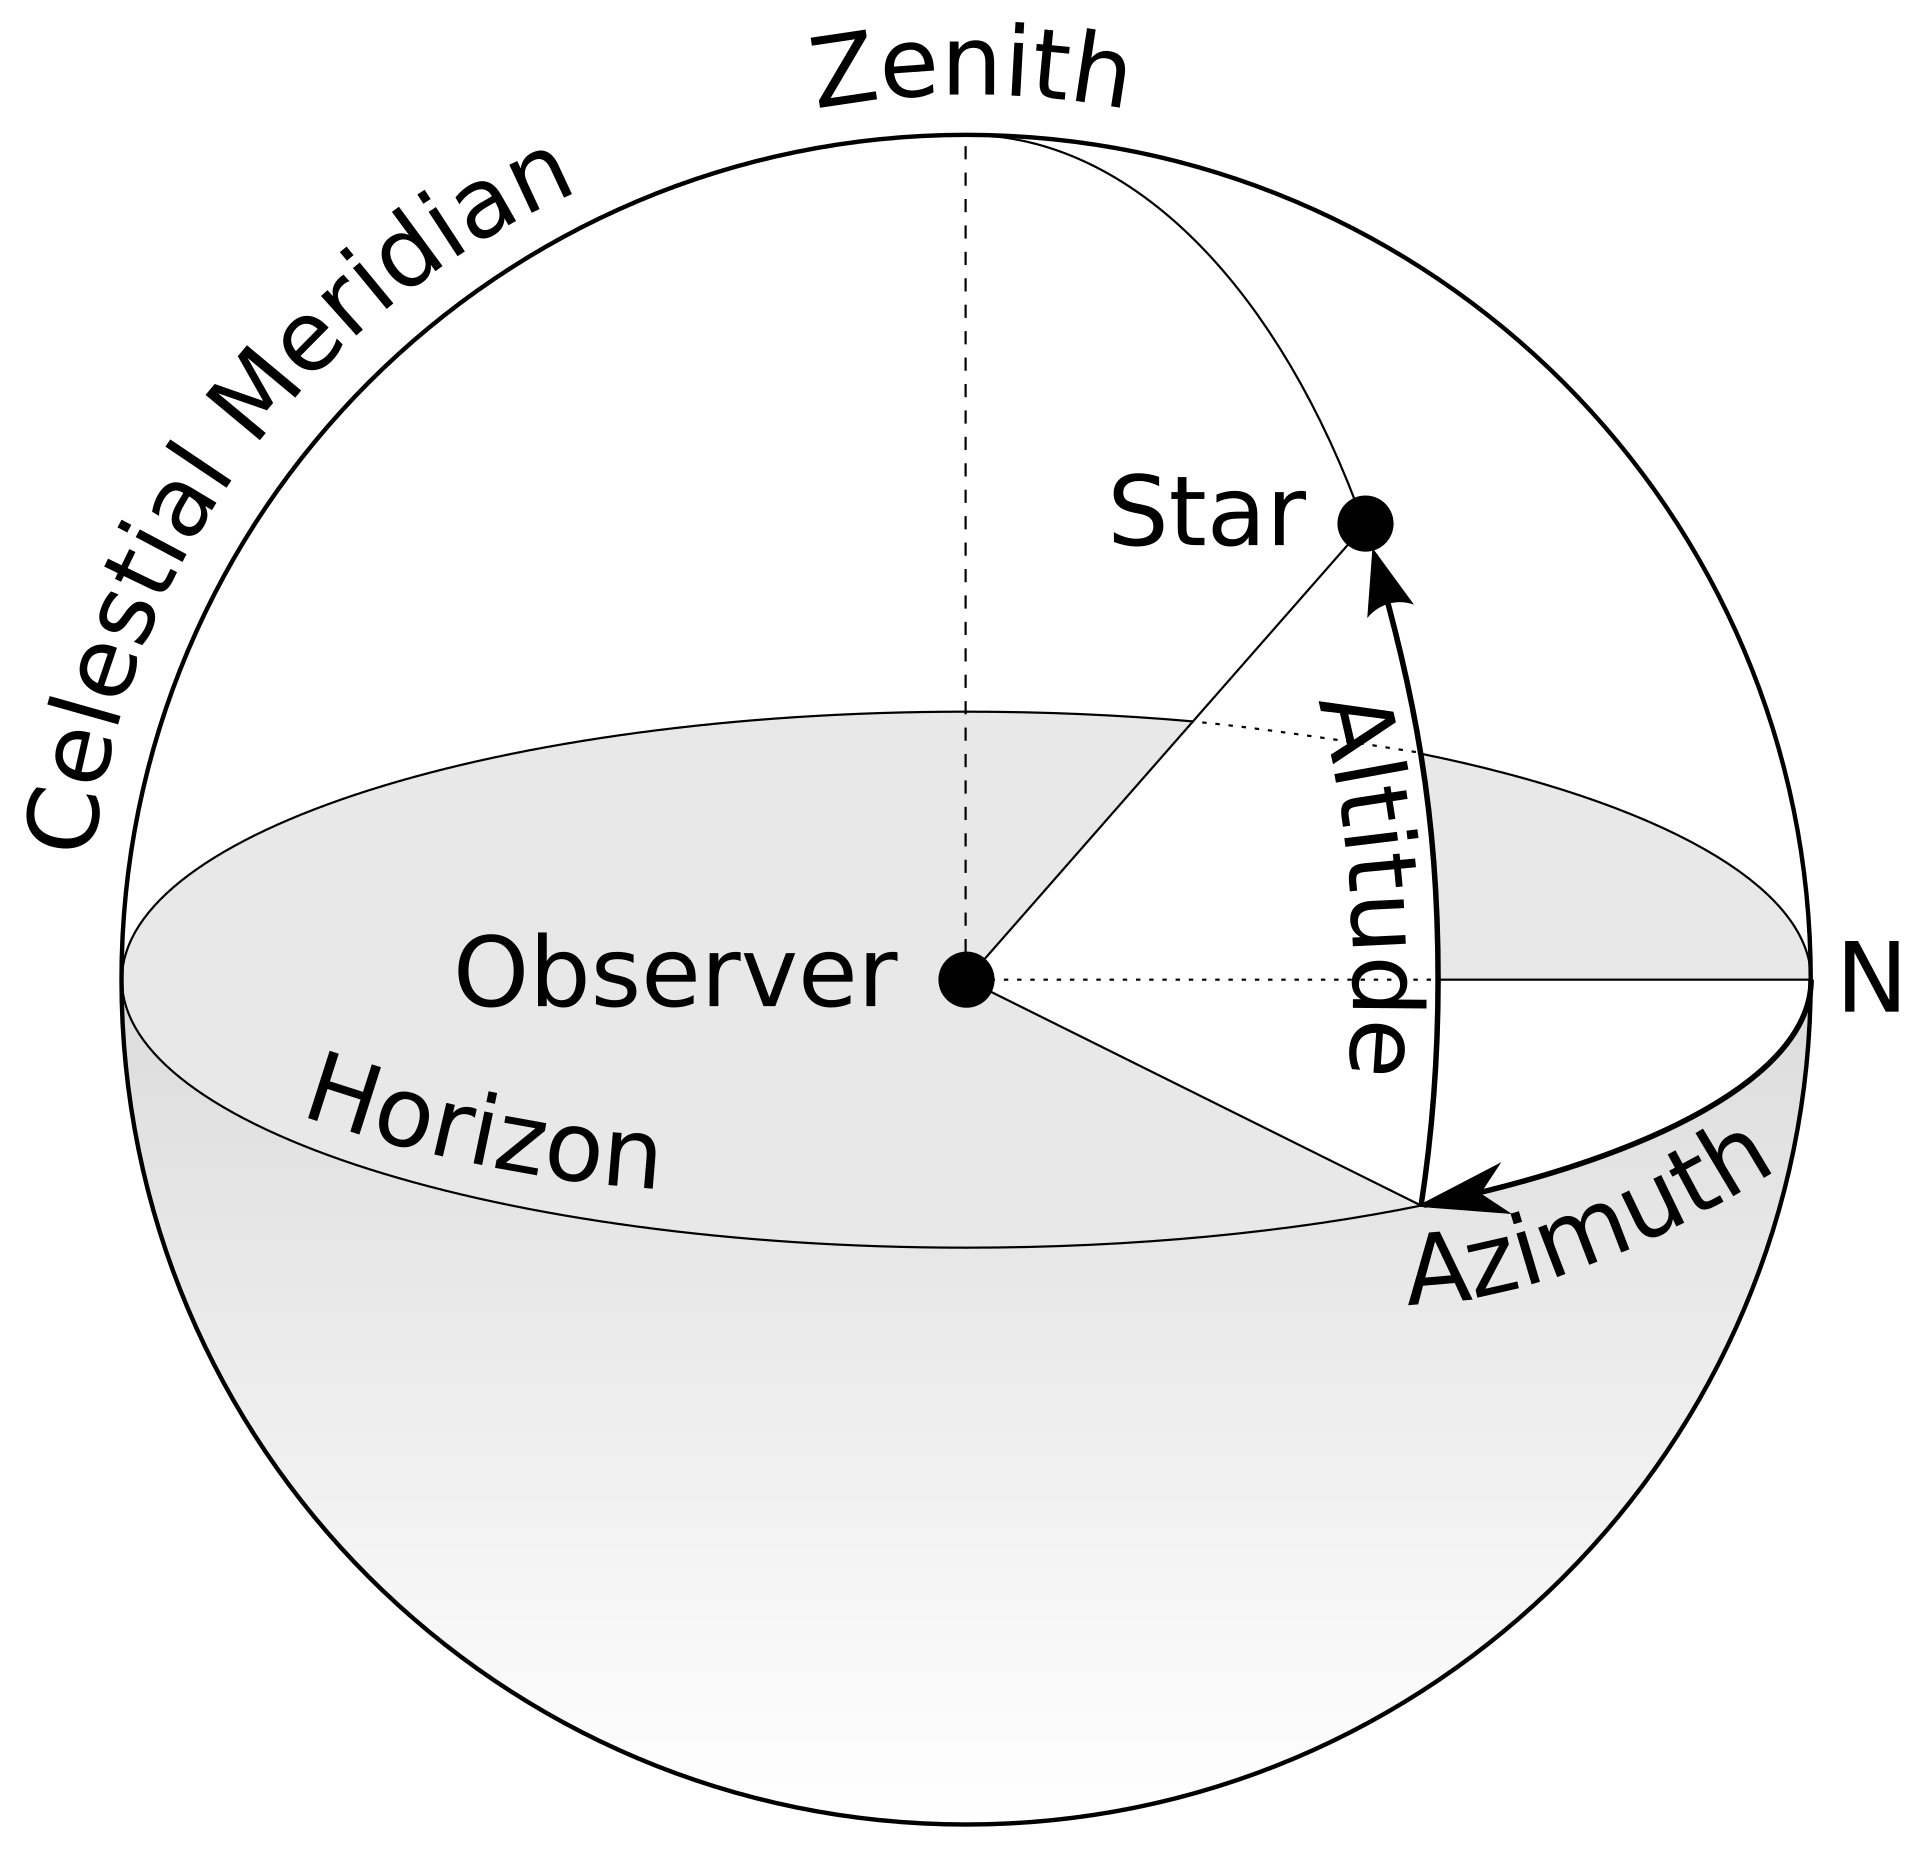
\includegraphics[width=0.6\textwidth]{Astronomy/Azimuth-Altitude_schematic.png}
    \caption[Altitude-azimuth coordinate system]{The altitude-azimuth coordinate system used at APEX. Source \cite{altazschematic}}
    \label{fig:altaz_coords}
\end{figure}




\subsection{Radio/(Sub)-mm Telescope Basics}
In this section, we present an overview of the fundamental components of a radio/(sub)-mm telescope.
As illustrated in Figure \ref{subfig:radio_telescope}, the basic operation of a Nasmyth-Cassegrain telescope design involves collecting electromagnetic radiation with a primary mirror, which is then reflected onto a secondary mirror (subreflector).
The photons are subsequently redirected toward the interior of the telescope, where they are converted into an electrical signal by an attached receiver (instrument).
The electric signal is then processed and recorded for further analysis.

Additionally, Figure \ref{subfig:beamwidth} provides a visual representation of the telescope's beam.
The telescope's beam indicates the source of the strongest signal detected by the telescope.
The beam power weakens towards the edges, and the goal is to place the source as the peak of the telescope's response, i.e., at the center of the beam
The angular resolution of a telescope, or the solid angle it can observe, is determined by the width of its beam.
Physical characteristics, including the primary dish diameter and the electromagnetic radiation frequency, determine the beam's width.
The standard measure for beamwidth is the half-power beamwidth or the angle between two points on the beam where the radiation power is half its maximum \cite{ToolsOfAst2009}.


% \section{Problem description}
% \textcolor{red}{This section have to be fixed completely}
% A telescope makes high precision observations of objects located very far away from Earth.
% Because of this distance, small changes such as the deformation of mirrors due to temperature might impact the precision drastically.\cc{Claudia Cicone: Here you could explain that astronomical objects are observed as they were "projected" in 2D angular coordinates on the sky, and you could talk about astronomical coordinates (see Lecture 5 notes of my course AST2210 for some explanation and references)
% }
% Over time, these deformations have been observed and analyzed, and in order to counter this, a pointing model is made.
% \cc{Claudia Cicone: The need for a pointing model is relevant mainly to sub-mm telescopes that cannot take real-time images of what they are observing, and so the precision of the pointing direction must be known accurately before starting the observations.}
% The pointing model uses measurements from various instruments and is fitted to the observed offsets.
% The model is used for about a month, or until it start performing poorly.
% The variation in measurements are still too big using only this model, so pointing scans have to be made regularly to correct even more.
% A pointing scan is an observation of an object with known location.
% When doing this, the offset on this observation is then added on top of the pointing model.
% These corrections to azimuth and elevations are used for a couple of hours, until a new pointing scan is made.
% \cc{Claudia Cicone: Need to define azimuth and elevation first, see other comment above
% }
% Using this approach, pointing error is reduced to about $4$ arc seconds.\\

% The aim of this thesis is to investigate the possibility of using machine learning to increase the performance of the telescope, by improving pointing accuracy.
% This can be done in multiple ways.

% One possibility is to apply a pointing model on top of the current pointing model using machine learning, such that the average offset is reduced even more.
% Another possibility is investigating the use of machine learning models to aid such that a pointing scan doesn't have to be made as often.
% This will reduce the workload at the telescope. \\


\part{Background and Theory}
\chapter{APEX Pointing Model and Database}
\section{Pointing model}\label{sec:pt_model}
Since radio/(sub)-mm telescopes observe over an extended time, they need a pointing model to obtain sufficiently accurate pointings.
The flux of the brightest radio sources is also weaker than the atmospheric emission,
which means that the signal is often hidden in the noise and needs to be extracted using long integrations and modulation techniques.
Therefore, astronomers must know that the pointing is accurate before initiating a long integration on the source.

The pointing model at APEX consists of two steps, an analytical model and additional pointing corrections performed at regular intervals based on recently observed pointing offsets.
The analytical model consists of fitting multiple terms to the many measurements of the pointing offset (difference between input coordinates and the observed coordinates of the source).
These terms can be geometric terms or terms related to, for example, metrology data.
The fitted terms are used for $1$-$2$ months and run in the background adjusting all input coordinates.
The additional pointing corrections are performed by astronomers every $1$-$2$ hours during the science observations and before observing a new target.

These equations explain the resulting pointing

\begin{align}
    Az &= Az_\text{input} + \Delta Az_\text{analytical model} + \Delta Az_\text{correction} \\ 
    El &= El_\text{input} + \Delta El_\text{analytical model} + \Delta El_\text{correction}
\end{align}
Where the first terms, $Az_\text{input}$ and $El_\text{input}$, are the input coordinates.
The second terms $\Delta Az_\text{analytical model}$ and $\Delta El_\text{analytical model}$ are the adjustment made according to the analytical model.
Furthermore, the last terms, $\Delta Az_\text{correction}$ and $\Delta El_\text{correction}$, are the corrections based on recently measured pointing offsets.

In the following section, we introduce and explain the adjustments from the analytical model and pointing offsets. 


\subsection{Analytical Model}

Accurately measuring pointing offsets without a pointing model can be challenging as the error is typically larger than the beamwidth, causing the source to fall outside the beam. At APEX,
astronomers use an optical receiver mounted in the primary mirror to make the initial observations, which allows them to observe the source in real-time.
During this process, which the astronomers perform periodically every $1$-$2$ months, the telescope is pointed at various sources with known locations, yielding both input and observed coordinates.

The analytical pointing model at APEX considers various factors that affect pointing, including purely geometrical terms based on the imperfect mounting of telescope components and empirical terms.
It uses the terms described below, all of which are dependent on the azimuth $Az$ or elevation $El$, except for a couple of constant terms.
The coefficients for all the terms are determined by the \texttt{TPOINT} \cite{tpoint_manual} software, using a linear fit based on the observed offsets from a pointing campaign.
The sum of all terms is the adjustment made by the model.

Most of the terms described in this section are fitted on data collected from the optical receiver mounted in the primary mirror.
Then, the astronomers refine the terms using observations from different instruments to develop specialized pointing models for each, while most terms remain constant from the optical fit.
The analytical model is crucial in accurately determining the telescope's pointing offsets, essential in obtaining high-quality observational data.
Table \ref{tab:analytical_terms} provides a list of the terms utilized in the analytical model,
indicating whether each term is determined through optical data or recalibrated for individual radio receivers.

The following descriptions of the terms are taken directly from the \texttt{TPOINT} software manual \cite{tpoint_manual}.
\subsubsection{Harmonic terms}
The analytical model has multiple harmonic terms, some geometrical and some empirical.
We introduce all the purely geometrical terms below, being AN, AW, CA, IA, IE, and NPAE, in addition to NRX, which is not purely geometrical but still affects pointing accuracy.
The \texttt{TPOINT} software that the APEX staff uses to develop the analytical model suggests terms that improve the model's performance on the chosen dataset.
The following terms are the empirical terms for azimuth.
\begin{align}\label{eq:analytical_az}
    \Delta Az =&  c_1 \cdot \sin{Az} + c_2 \cdot \frac{\cos{2Az}}{\cos{El}} + c_3 \cdot \cos{3Az} + c_4 \cdot \sin{2Az} \\
    &+ c_5 \cdot \cos{2Az} + c_6 \cdot \frac{\cos{Az}}{\cos{El}} + c_7 \cdot \frac{\cos{5Az}}{\cos{El}},
\end{align}
and the terms for elevation are

\begin{align}\label{eq:analytical_el}
    \Delta El =&  c_1 \cdot \sin{El} + c_2 \cdot \cos{El}+ c_3 \cdot \cos{2Az} + c_4 \cdot \sin{2Az} \\
    &+ c_5 \cdot \cos{3Az} + c_6 \cdot \sin{3Az} + c_7 \cdot \sin{4Az} + c_8 \cdot \sin{5Az}  
\end{align}


The \texttt{TPOINT} software denotes the harmonic terms in the format $Hrfci$. The list below explains the different terms.

\begin{itemize}
    \item $H$: Stands for harmonics
    \item $r$: The resulting variable, either $Az$ or $El$, denoting azimuth and elevation respectively.
    The resulting variable can also be $S$, which means the result is horizontal, or azimuth scaled by a factor $1/\cos{El}$.
    \item $f$: The harmonic function, either $S$ or $C$ denoting \textit{sine} and \textit{cosine}.
    \item $c$: The variable that the funciton $f$ is dependent on, either $Az$ or $El$.
    \item $i$: Integer value in the range $0$-$9$, denoting the frequency of the harmonic.
\end{itemize}

For example, is $\Delta Az = \text{HACA3}\cos{3Az}$ denoted as HACA3 in the \texttt{TPOINT} software.

\subsubsection{Az/El non-perpendicularity (NPAE)}
In an altazimuth mount, if the azimuth axis and elevation axis are not exactly at
right angles, horizontal shifts proportional to $\sin{El}$ occur. This effect is zero when pointing at the horizon and increases with elevation proportional to $1/\cos{El}$

\begin{equation}
    \Delta Az \simeq - \text{NPAE } \frac{\sin{El}}{\cos{El}}= - \text{NPAE } \tan{El},
\end{equation}
where NPAE is the horizontal displacement when pointing at Zenith.

\subsubsection{Left-right collimation error (CA)}
In an altazimuth mount, the collimation error is the non-perpendicularity between the nominated pointing direction and the elevation axis.
It produces a horizontal image shift given by
\begin{equation}\label{eq:pmodel_ca}
    \Delta Az \simeq -\text{CA} / \cos{El}
\end{equation}


\subsubsection{Azimuth and elevation index error (IA/IE)}
Index errors are the errors when pointing at origo.

The azimuth index error is 
\begin{equation}
    \Delta Az = -\text{IA},
\end{equation}

and elevation index error is
\begin{equation}\label{eq:pmodel_ie}
    \Delta El = \text{IE}
\end{equation}

\subsubsection{Azimuth axis misalignment (AN/AW)} 

In an altazimuth mount, misalignment of the azimuth axis north-south or east-west causes errors.
The errors caused by misalignment in the north-south are given by

\begin{equation}
    \Delta Az \simeq - \text{AN} \sin{Az} \cdot \tan{El},
\end{equation}

and

\begin{equation}
    \Delta El \simeq - \text{AN} \cos{Az},
\end{equation}
where AN is the misalignment alignment in the north-south direction.
The errors given by misalignment in east-west are given by

\begin{equation}
    \Delta Az \simeq - \text{AW} \cos{Az} \tan{El},
\end{equation}

and

\begin{equation}
    \Delta El \simeq \text{AW} \sin{Az},
\end{equation}
where AW is the misalignment alignment in the east-west direction.

\subsubsection{Horizontal displacement of Nasmyth rotator (NRX)}
In a Nasmyth altazimuth mount, a horizontal displacement between the elevation axis of the mount and the rotation axis of the Nasmyth instrument-rotator produces
and image shift on the sky with a horizontal component
\begin{equation}
    \Delta Az \simeq - \text{NRX},
\end{equation}
and an elevation component
\begin{equation}
    \Delta El \simeq - \text{NRX} \sin{El},
\end{equation}
where NRX is the horizontal displacement.




\begin{table}[!htbp]
    \centering
    \caption[List of terms in the analytical pointing model at APEX]{List of terms included in the analytical pointing model at APEX.
    All the terms are fitted using observations from the optical receiver,
    while the terms below "Radio receiver" are refitted specifically for each radio receiver. }
    \begin{tabular}{lcc}
        \toprule
    \textbf{Term} & \textbf{Azimuth} & \textbf{Elevation} \\
    \hline
    \multicolumn{3}{c}{Optical receiver} \\ 
    \hline
    NPAE  & x &  \\
    HASA  & x &  \\
    HECA2 &  & x \\
    HSCA2 & x &  \\
    HACA3 & x &  \\
    HASA2 & x &  \\
    HACA2 & x &  \\
    HSCA  & x &  \\
    HESA2 &  & x \\
    HECA3 &  & x \\
    HSCA5 & x &  \\
    HESA3 &  & x \\
    HESA4 &  & x \\
    HESA5 &  & x \\
    NRX   & x & x \\
    NRY   & x & x \\
    \hline
    \multicolumn{3}{c}{Radio receivers} \\
    \hline
    HESE  &  & x \\
    HECE  &  & x \\
    IA    & x &  \\
    IE    &  & x \\
    CA    & x &  \\
    AN    & x & x \\
    AW    & x & x \\
    \bottomrule 
    \end{tabular}
    \label{tab:analytical_terms}
\end{table}


\subsection{Pointing Corrections} 
Although the analytical linear regression pointing model at APEX fits pointing campaign observations well,
it cannot accurately model the changes in pointing over time, resulting in residual errors.
Astronomers regularly correct these errors by observing a strong source with known coordinates,
measuring the pointing offset, and updating the model's terms for azimuth and elevation correction (CA and IE, respectively).
The update procedure is as follows:
\begin{align}
    \text{CA} &= \text{CA} + \delta_{\text{Az}} \label{eq:ca}\\ 
    \text{IE} &= \text{IE} - \delta_{\text{El}},\label{eq:ie}
\end{align}
where $\delta_{\text{Az}}$ and $\delta_{\text{El}}$ are the recently observed pointing offsets in azimuth and elevation, respectively.
The astronomers perform these pointing corrections every couple of hours to ensure the pointing is sufficient during science observations.

Note that we divide the term CA \eqref{eq:pmodel_ca} by cosine elevation, which converts the observed horizontal offset to azimuth.

\section{APEX Database} \label{sec:database}
In this section, we introduce the different data sources utilized throughout the research in this thesis.


\subsection{Pointing Scan Data}
During a pointing scan, the telescope observes a source with a known location to obtain a pointing offset measured in arcseconds.
The observers use this offset to correct the pointing model (using equations \eqref{eq:ca} and \eqref{eq:ie}).
There are two types of pointing scans: Line-pointings and continuum scans.

\subsubsection{Line-pointing}
A line-pointing involves pointing at an extended source. 
The telescope then makes ten scans, recording the flux intensity from the source, five vertically and five horizontally,
around the center of the pointing, as shown in figure \ref{fig:line_pointings}.
The upper panel shows a high-quality pointing scan, and the lower panel shows a noisy, low-quality pointing scan.
The cross-plot on the right side shows the line spectrum for each observation (center plus eight offset observations).

The integrals of the flux recorded from the source are plotted as blue dots on the left-hand side of the panel.
A Gaussian is fitted to these points, and the table shows the resulting amplitude, full width at half maximum (FWHM), and offsets.

\begin{figure}[H]
    \centering
     \begin{subfigure}[b]{0.75\textwidth}
         \centering
         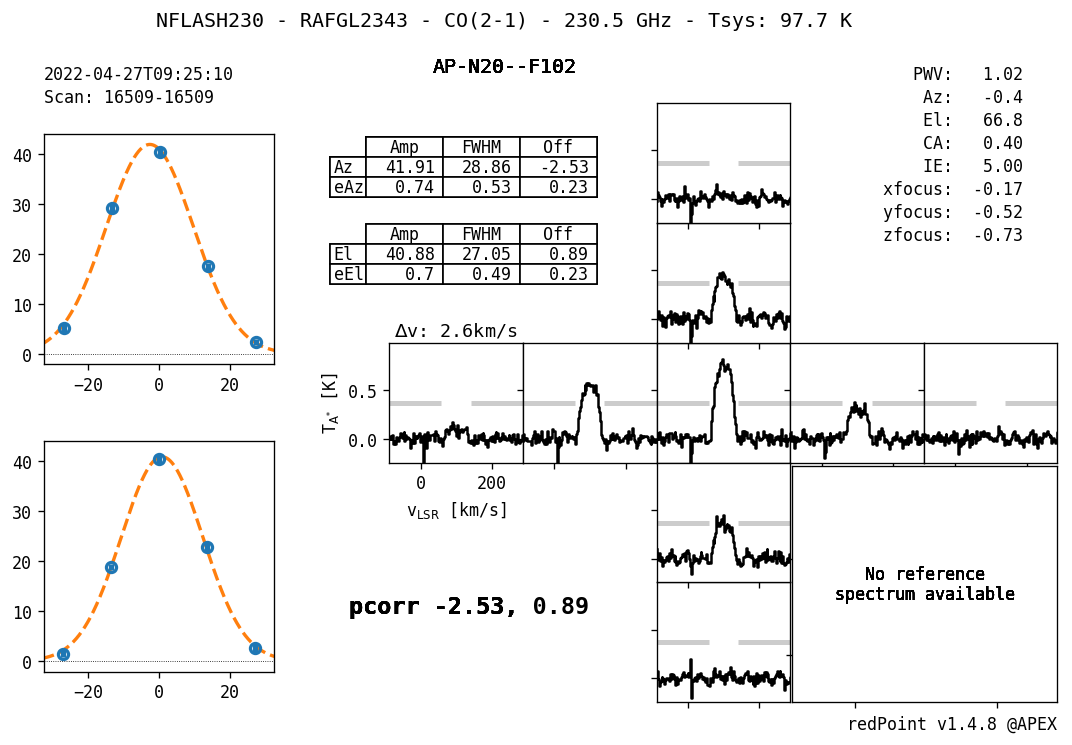
\includegraphics[width=\textwidth]{Pointing Scans/good_line.png}
         \caption{Line-pointing with little noise and a good Gaussian fit.}
         \label{subfig:good_line}
     \end{subfigure}
    \\
     \begin{subfigure}[b]{0.75\textwidth}
         \centering
         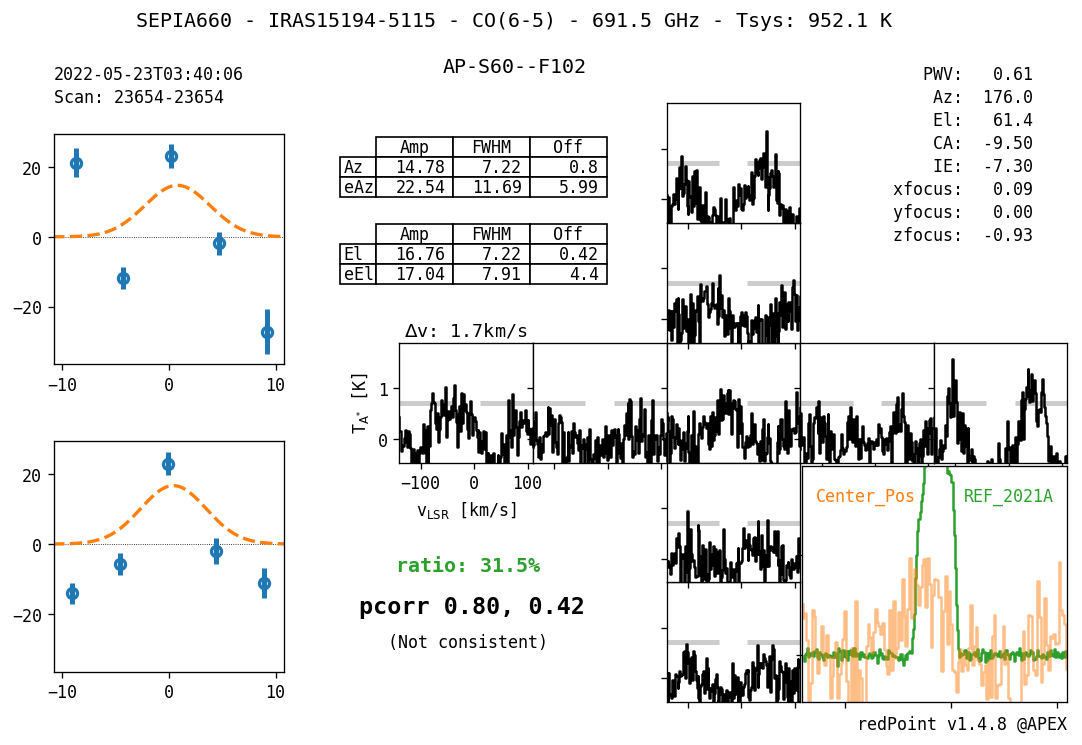
\includegraphics[width=\textwidth]{Pointing Scans/bad_line.png}
         \caption{Noisy line-pointing with bad Gaussian fit.}
         \label{subfig:bad_line}
     \end{subfigure}
    \caption[Line pointing panel]{The two figures show line-pointing scans. a) is good and clean, and b) is noisy and unreliable. A Gaussian is fit both for the azimuth and elevation pointing.
    The table shows the amplitude, full width at half maximum (FWHM), offset, and the uncertainty of these measures, for azimuth and elevation.
    The figures also show the correction applied during the pointing ($ca$ and $ie$), along with other metrics.}
    \label{fig:line_pointings}
\end{figure}

\subsubsection{Continuum Scan}
Not all sources have emission lines; for these sources, the telescope performs a continuum scan instead. In this case, a source is continuously scanned in azimuth and elevation while recording the flux intensity.
A Gaussian curve is fitted to the recorded flux intensity to determine the offsets, amplitude, and full width at half maximum (FWHM).
Figure \ref{fig:continueous_pointings} show examples of continuum scans and the corresponding Gaussian fits.

\begin{figure}[H]
    \centering
     \begin{subfigure}[b]{0.75\textwidth}
         \centering
         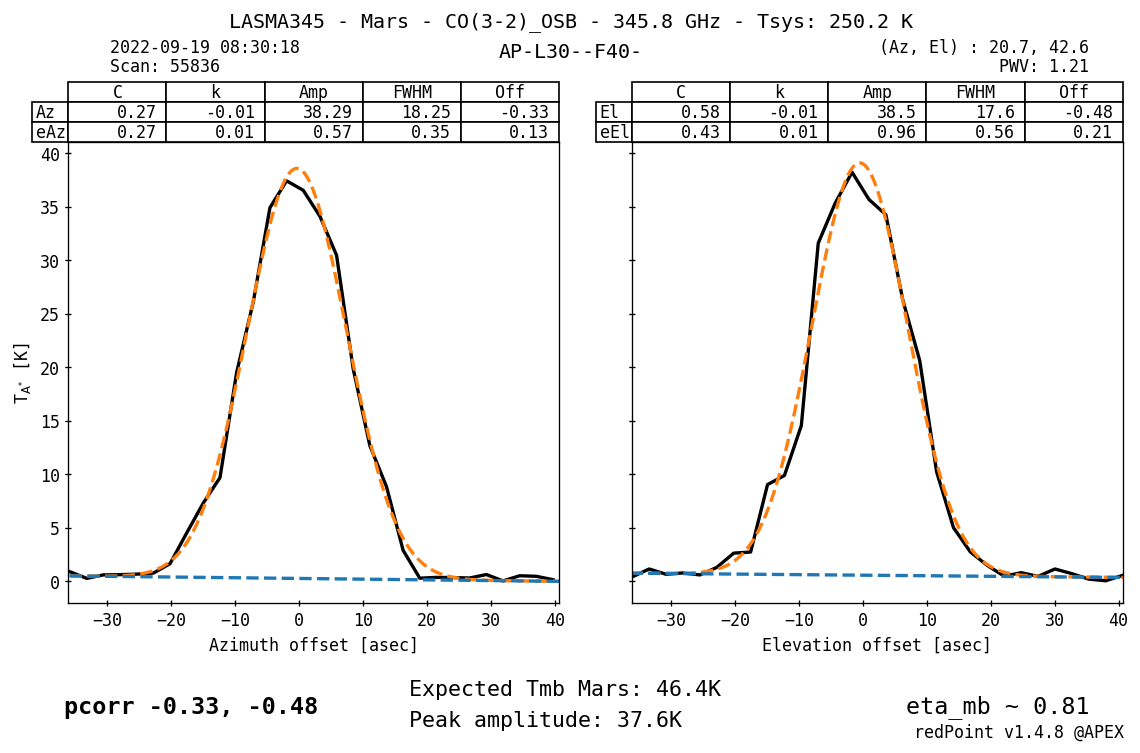
\includegraphics[width=\textwidth]{Pointing Scans/good_continuous.png}
         \caption{Line-pointing with little noise and a good Gaussian fit.}
         \label{subfig:good_continuous}
     \end{subfigure}
    \\
     \begin{subfigure}[b]{0.75\textwidth}
         \centering
         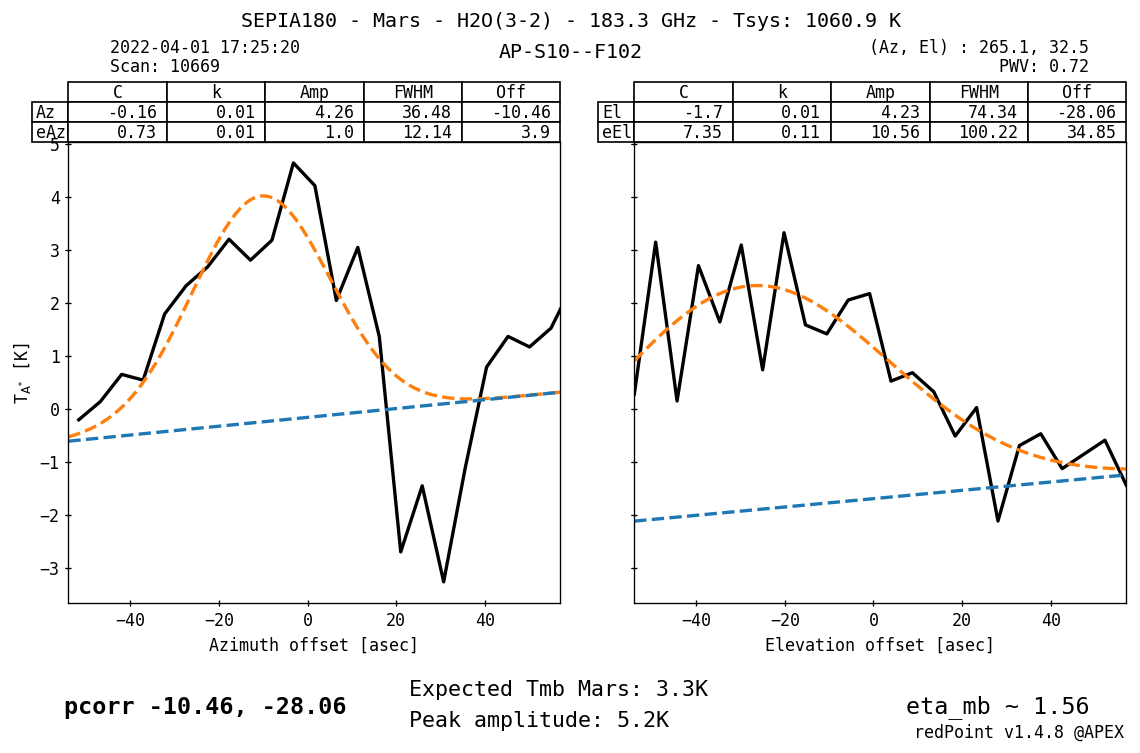
\includegraphics[width=\textwidth]{Pointing Scans/bad_continuous.png}
         \caption{Noisy line-pointing with bad Gaussian fit.}
         \label{subfig:bad_continuous}
     \end{subfigure}
    \caption[Continuum scan panel]{The two panels show continuum pointing scans. a) is good and clean, and b) is noisy and unreliable. 
    A Gaussian is fit both for the azimuth and elevation pointing. The amplitude, full width at half maximum, offset, and the uncertainty of these measures are shown for both of the fits.}
    \label{fig:continueous_pointings}
\end{figure}



\subsubsection{Pointing scan timestamp} 
In the main database, each pointing scan has a timestamp in the format YYYY-MM-DD HH:MM:SS, with a one-second resolution.
This timestamp does not reflect the actual start of a pointing scan.
Also, no information in the database itself indicates whether the telescope is observing, but this information can be extracted from some dump files from the tiltmeter, which includes a flag indicating whether the telescope is idle, preparing to observe, or observing.
Combining this flag with the timestamps, we can obtain the accurate start and end time of a pointing scan. However, these tiltmeter dump files are only available for some time periods.

\subsubsection{Instruments}
The observing instruments on the telescope operate at various frequencies.
Table \ref{tab:instrument_usage} provides information on the frequency range covered by each instrument,
along with the number of scans performed using each instrument throughout the year 2022.\\

The broad range of frequencies at which astronomical phenomena emit electromagnetic radiation requires observation across a wide range of frequencies to study these phenomena comprehensively.
APEX's \href{https://www.eso.org/sci/facilities/apex/cfp/cfp110/instrument_summary.html.html}{website} provides a complete list of instruments along with their descriptions.
\begin{table}[H]
    \centering
    \caption[Number of scans for each instrument]{The number of times each instrument was used for a pointing scan in $2022$. There are $8847$ scans in total.}
    \begin{tabular}{lcr}
        \toprule
        Instrument & Frequency band [GHz] &\# of scans \\
        \midrule
        NFLASH230 & $200$-$270$ &3197 \\
        LASMA345  & $268$-$375$ &1861 \\
        NFLASH460 & $385$-$500$ &1394 \\
        SEPIA660  & $578$-$738$ & 856 \\
        SEPIA345  & $272$-$376$ & 818 \\
        SEPIA180  & $159$-$211$ & 359 \\
        HOLO      & - & 225 \\
        ZEUS2     & - & 103 \\
        CHAMP690  & - &  34 \\
        \bottomrule
        \end{tabular}
        \label{tab:instrument_usage}
\end{table}



\subsection{The Monitor Database}
The monitor database is critical in this project, providing valuable sensory data from within and outside the telescope.
In this section, we will explore the data contained within the monitor database and identify the most relevant variables to our purposes.
We had a copy of the database containing data from 01.01.2022 to 17.09.2022.

The monitor database provides data with varying frequencies, as shown in Table \ref{tab:data_frequency},
which lists the approximate number of data points per minute for each table used in this project.
Figure \ref{fig:features_during_scans} presents scatter plots of a selected subset of variables from the database during pointing scans.  

\subsubsection{Azimuth and Elevation}
The database includes tables for the input azimuth and elevation, labeled COMMANDAZ and COMMANDEL.
These tables contain the raw coordinates before the pointing model has adjusted the pointing.

The database also includes tables for the actual azimuth and elevation, labeled ACTUALAZ and ACTUALEL.
These tables contain the coordinates obtained after applying the pointing model and automatic adjustments based on sensory data.

Finally, the database contains tables for the azimuth and elevation velocity, labeled ACTUALVELOCITYAZ and ACTUALVELOCITYEL.
These tables provide information on the velocity of the telescope during observations.

The frequency of these measurements is $6$ data points per minute.
Figure \ref{subfig:scan_az} show these measurements for the duration of a pointing scan, along with additional data points before and after the scan.


\subsubsection{Temperature Measurements}
Multiple instruments located at different locations on the telescope measure the temperature and store the measurements in the database.
The tables that contain these measurements are labeled TEMPERATURE, TEMP1 through TEMP6, TEMP26 through TEMP28, and TILT1T. 
Figure \ref{fig:corr_temp} indicates that many of these measurements are highly correlated.
For example, TEMP1 through TEMP6 show a strong correlation $\geq 0.98$.
Similarly, TEMP26 through TEMP28 and TEMPERATURE are also highly correlated.
The frequencies of some of these measurements are different, and they may all be found in Table \ref{tab:data_frequency}.
Figure \ref{subfig:scan_temp1} and \ref{subfig:scan_tilt1t} show the measurements of TEMP1 and TILT1T respectively
for the duration of a pointing scan and additional data points before and after the scan.


\begin{figure}[H]
    \centering
    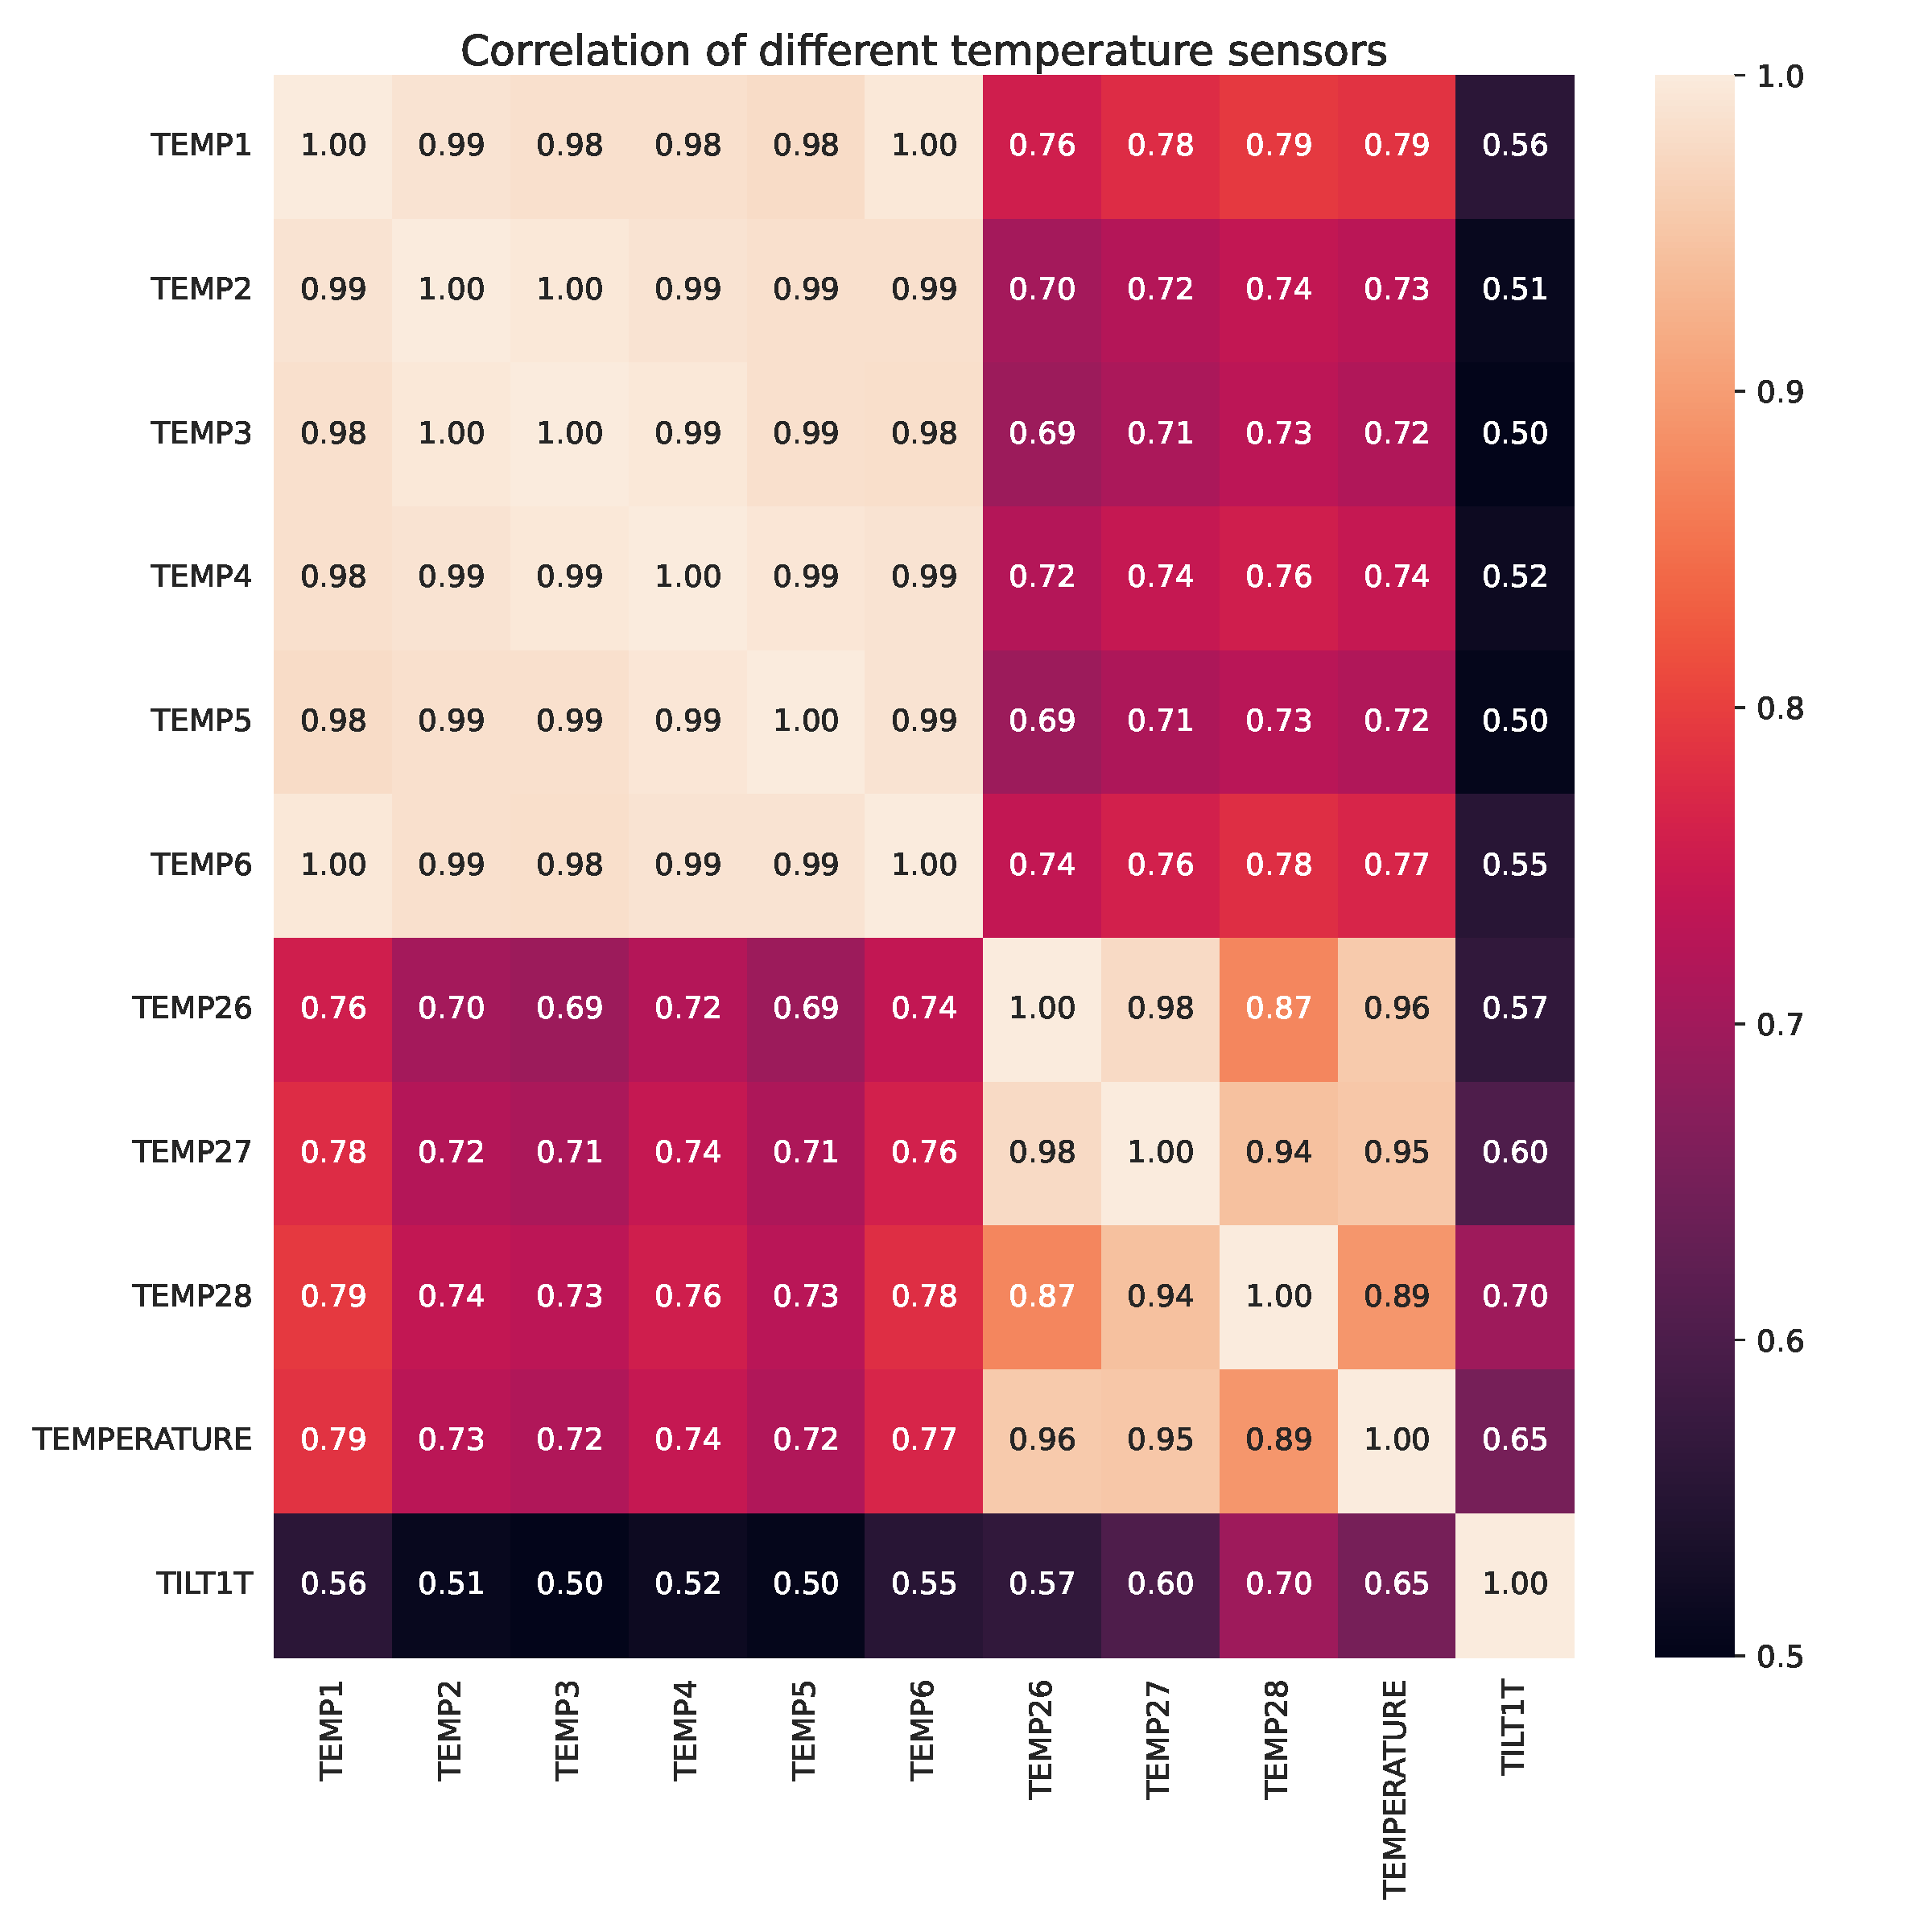
\includegraphics[width=0.98\textwidth]{Correlation/Correlation_temp.pdf}
    \caption[Correlation between temperature measurements]{Linear correlation between temperature measurements at APEX.
    The values are sampled by the median value at each pointing scan.}
    \label{fig:corr_temp}
\end{figure}

\subsubsection{Hexapod}
The secondary mirror, also known as the subreflector, is supported by a hexapod.
The hexapod moves in three dimensions and rotates around azimuth and elevation axes.
There are five measures associated with the hexapod: POSITIONX, POSITIONY, POSITIONZ, ROTATIONX, and ROTATIONY.
These measures are essential for positioning the secondary mirror and ensuring accurate pointing.
The frequency of these measurements is $6$ data points per minute.

\subsubsection{Tiltmeter}
The telescope has two tiltmeters that measure its tilt or inclination to the vertical direction.
One tiltmeter aligns with the telescope's pointing (TILT1X), while the other is orthogonal to the pointing (TILT1Y).
The frequency of these measurements is $12$ data points per minute.

\subsubsection{Weather data}
The weather station at the telescope provides measurements of various weather parameters, including dew point, humidity, pressure, wind speed, and wind direction.
The instruments take measurements at a frequency of $5$ data points per minute.
The figures \ref{subfig:scan_winddir} and \ref{subfig:scan_windspeed} show wind direction and speed measurements for the time period around a pointing scan.


\subsubsection{Disp abs?}

Frequency of $12$ data points per minute.

\subsubsection{Automatic adjustments}
Automatic adjustments based on readings from various sensors ensure accurate and stable pointing of the telescope.
These adjustments account for previously modeled systematic errors based on measurements from tiltmeters, temperature sensors installed at different locations, and other relevant data sources.
Some system at the telescope automatically makes these adjustments, and the tables in the database that contain information about these adjustments start with DAZ or DEL, denoting adjustments in azimuth and elevation, respectively.
The frequency of this data is $12$ data points per minute.
Table \ref{tab:data_frequency} shows a comprehensive list of these variables.

\begin{table}[H]
    \caption[Database frequencies]{The frequency in data points per minute of different variables in the monitor database.}
    \centering
    \begin{tabular}{lr}
        \toprule
        Table &  Frequency [datapoints/minute] \\
        \midrule
        ACTUALAZ &                    6 \\
        ACTUALEL &                    6 \\
        ACTUALVELOCITYAZ &                    6 \\
        ACTUALVELOCITYEL &                    6 \\
        COMMANDEL &                    6 \\
        COMMANDAZ &                    6 \\
        TILT1X &                   12 \\
        TILT2Y &                   12 \\
        TILT1T &                   12 \\
        TEMPERATURE &                    5 \\
        TEMP1 &                    6 \\
        TEMP2 &                    6 \\
        TEMP3 &                    6 \\
        TEMP4 &                    6 \\
        TEMP5 &                    6 \\
        TEMP6 &                    6 \\
        TEMP26 &                    2 \\
        TEMP27 &                    2 \\
        TEMP28 &                    2 \\
        DAZ\_TEMP &                   12 \\
        DAZ\_TILT &                   12 \\
        DAZ\_TILTTEMP &                   12 \\
        DAZ\_SPEM &                   12 \\
        DAZ\_DISP &                   12 \\
        DAZ\_TOTAL &                   12 \\
        DEL\_TEMP &                   12 \\
        DEL\_TILT &                   12 \\
        DEL\_TILTTEMP &                   12 \\
        DEL\_SPEM &                   12 \\
        DEL\_DISP &                   12 \\
        DEL\_TOTAL &                   12 \\
        POSITIONX &                    6 \\
        POSITIONY &                    6 \\
        POSITIONZ &                    6 \\
        ROTATIONX &                    6 \\
        ROTATIONY &                    6 \\
        DISP\_ABS1 &                   12 \\
        DISP\_ABS3 &                   12 \\
        DISP\_ABS2 &                   12 \\
        DEWPOINT &                    5 \\
        PRESSURE &                    5 \\
        HUMIDITY &                    5 \\
        WINDSPEED &                    5 \\
        WINDDIRECTION &                    5\\
        \bottomrule
    \end{tabular}
    \label{tab:data_frequency}
\end{table}


\begin{figure}[H]
    \centering
    \begin{subfigure}[t]{0.49\textwidth}
        \centering
        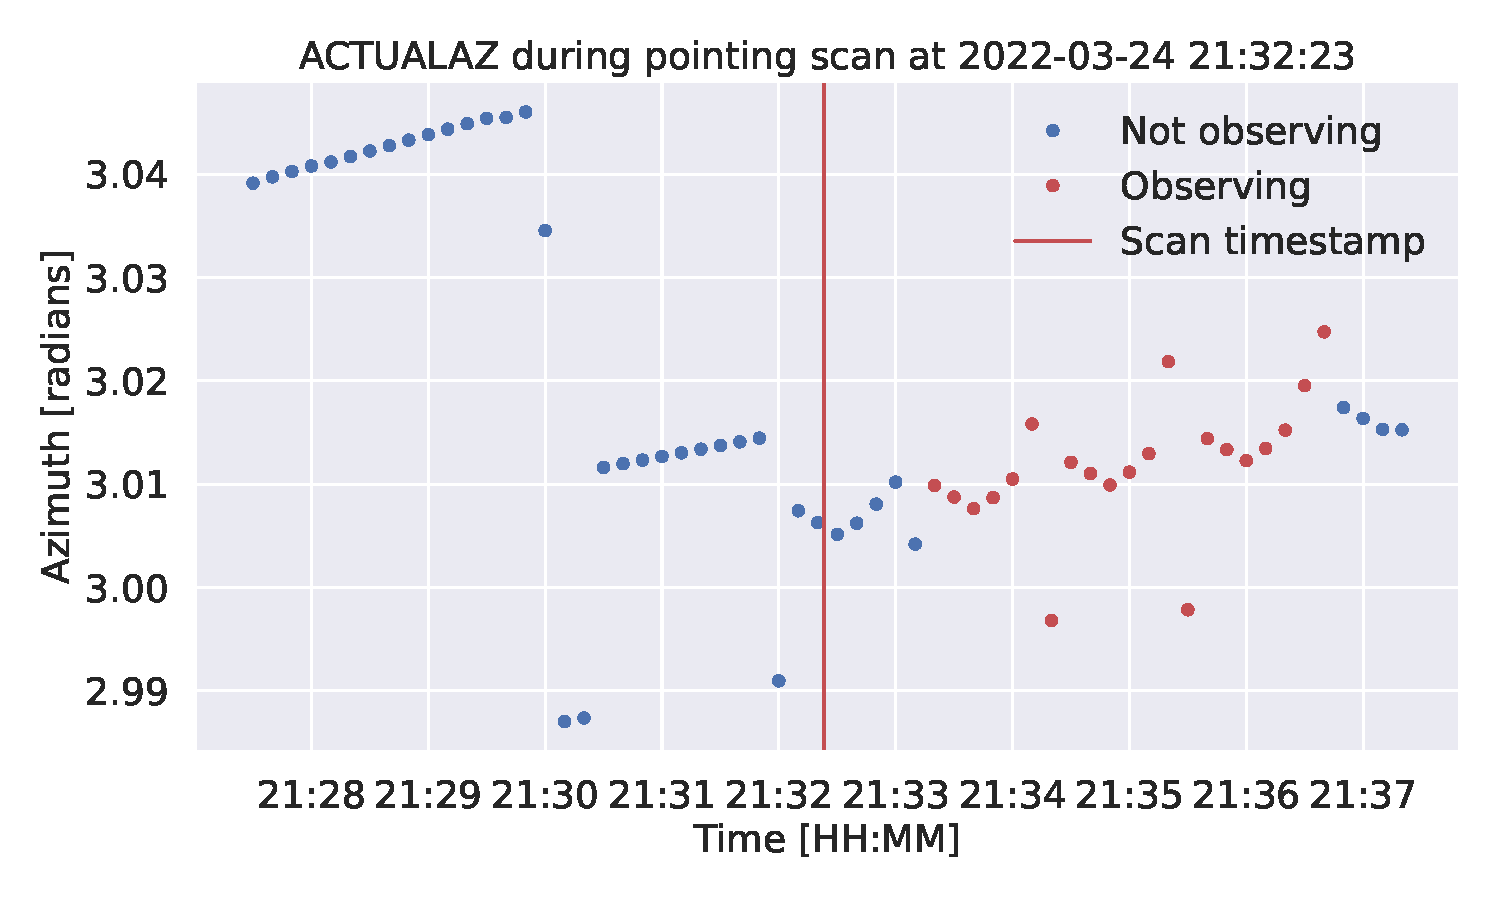
\includegraphics[width=\textwidth]{Feature during scans/scan_ACTUALAZ_335.pdf}
        \caption{Azimuth angle}
        \label{subfig:scan_az}
    \end{subfigure}
    \begin{subfigure}[t]{0.49\textwidth}
       \centering
       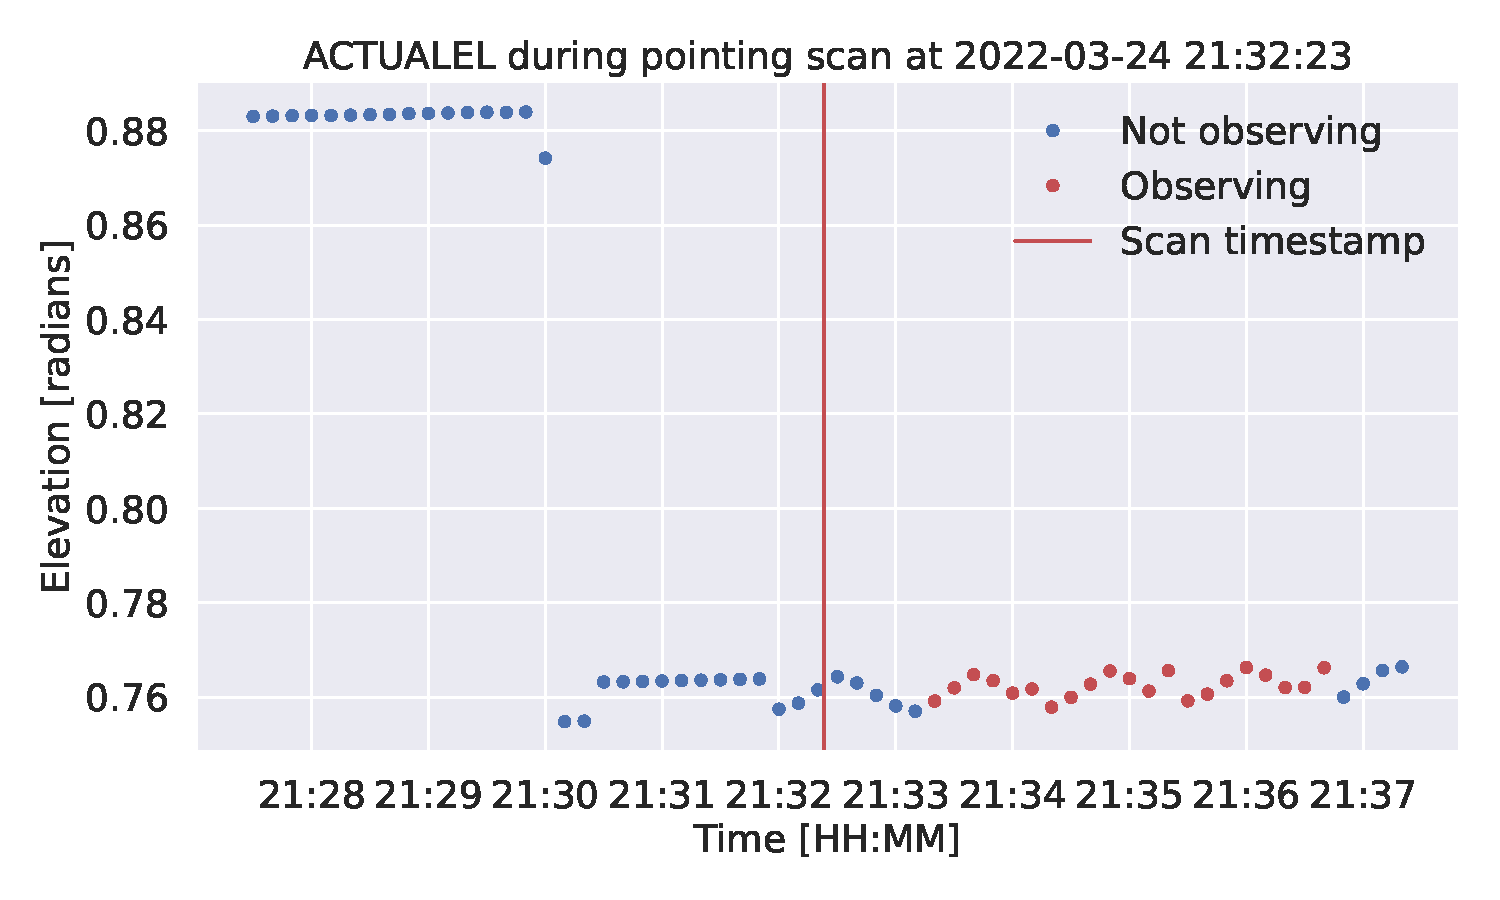
\includegraphics[width=1\textwidth]{Feature during scans/scan_ACTUALEL_335.pdf}
       \caption{Elevation angle.}
       \label{subfig:scan_el}
    \end{subfigure}
    \\~\\
    \begin{subfigure}[t]{0.49\textwidth}
        \centering
        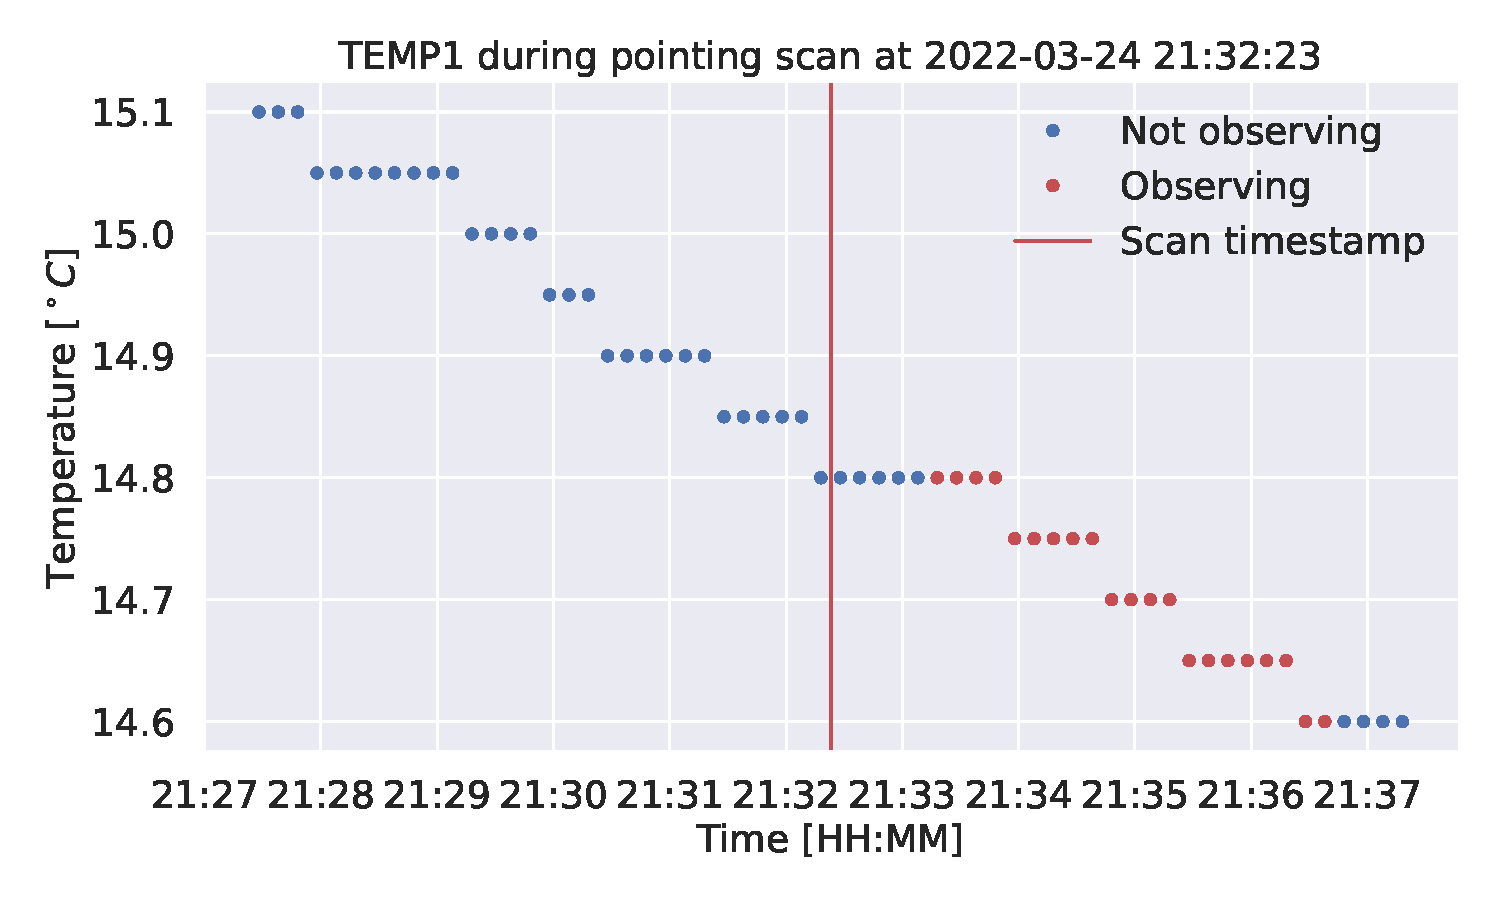
\includegraphics[width=\textwidth]{Feature during scans/scan_TEMP1_335.pdf}
        \caption{Temperature measurements at temperature sensor $1$.}
        \label{subfig:scan_temp1}
    \end{subfigure}
       \begin{subfigure}[t]{0.49\textwidth}
        \centering
        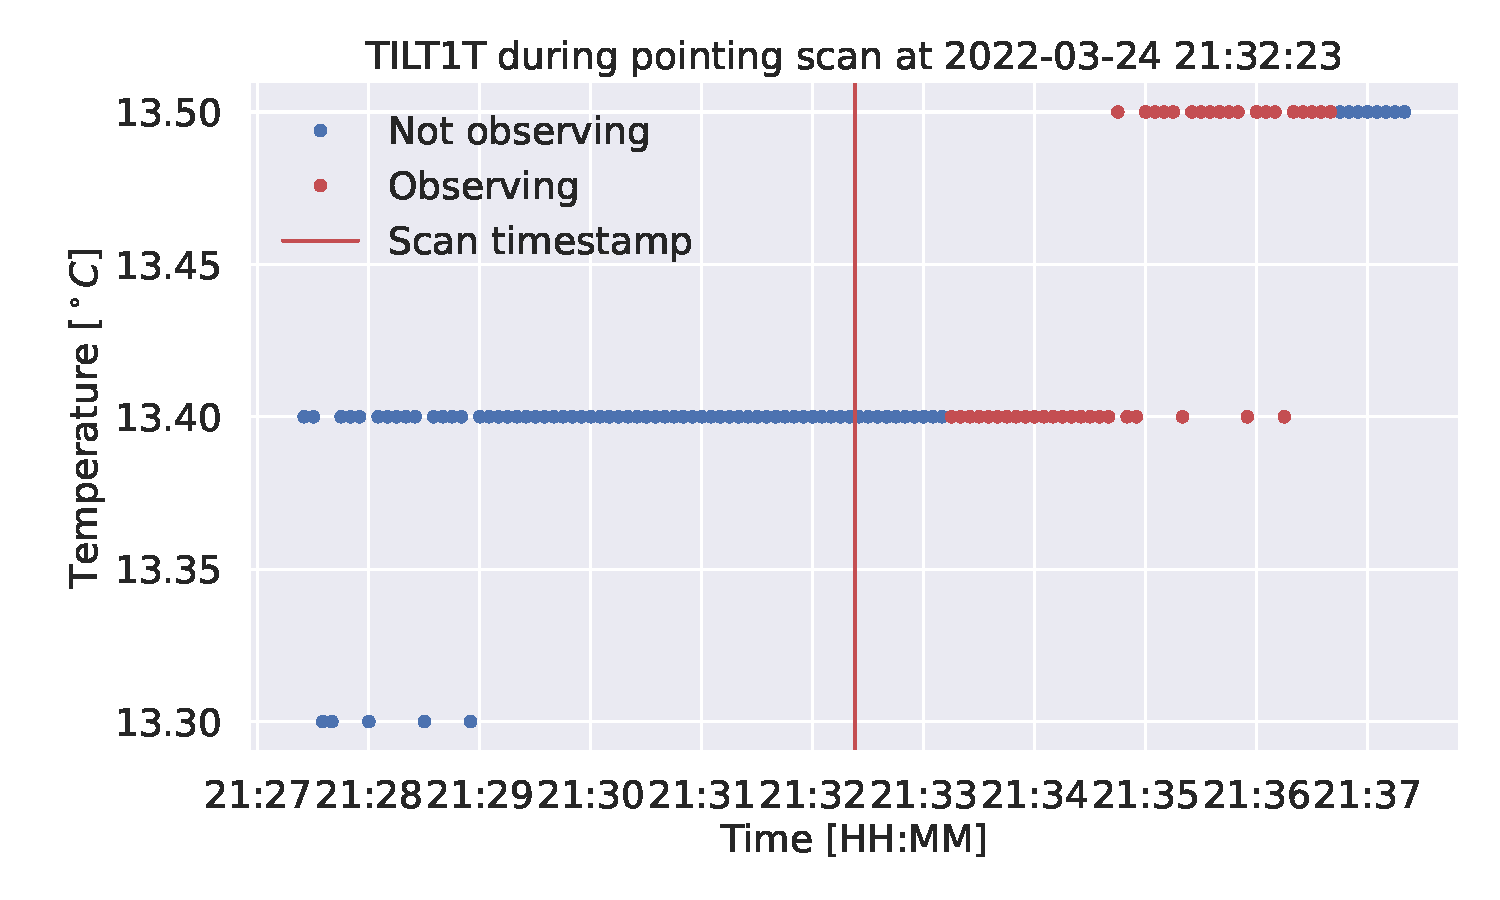
\includegraphics[width=\textwidth]{Feature during scans/scan_TILT1T_335.pdf}
        \caption{Temperature measurements at tiltmeter $1$.}
        \label{subfig:scan_tilt1t}
    \end{subfigure}
    \\~\\
    \begin{subfigure}[t]{0.49\textwidth}
        \centering
        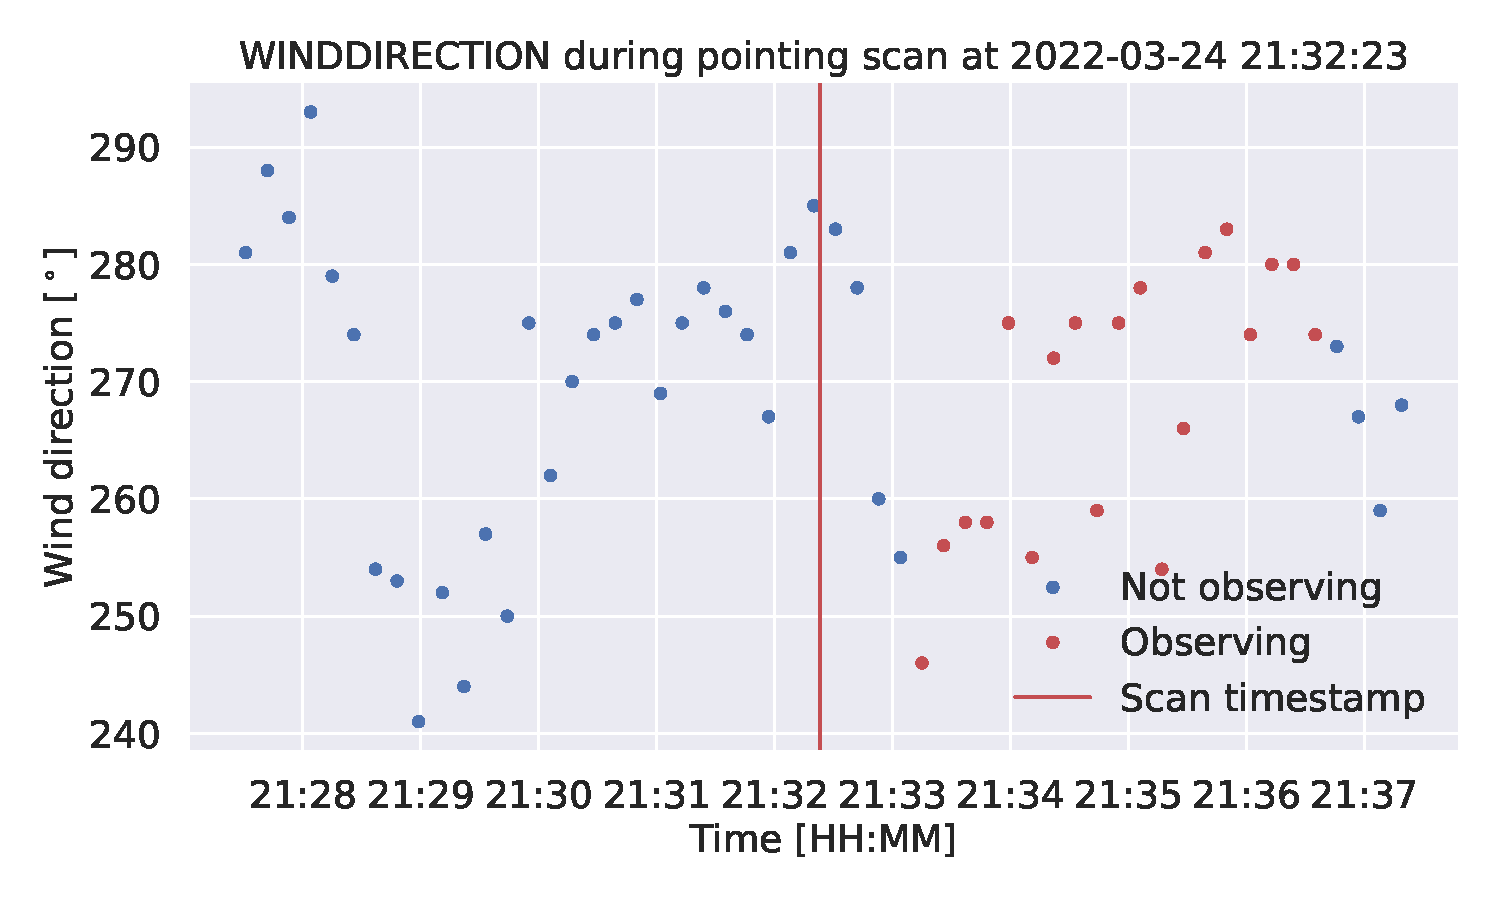
\includegraphics[width=\textwidth]{Feature during scans/scan_WINDDIRECTION_335.pdf}
        \caption{Wind direction data from the weather station, measured in degrees from North, where clockwise is the positive angle direction.}
        \label{subfig:scan_winddir}
    \end{subfigure}
       \begin{subfigure}[t]{0.49\textwidth}
        \centering
        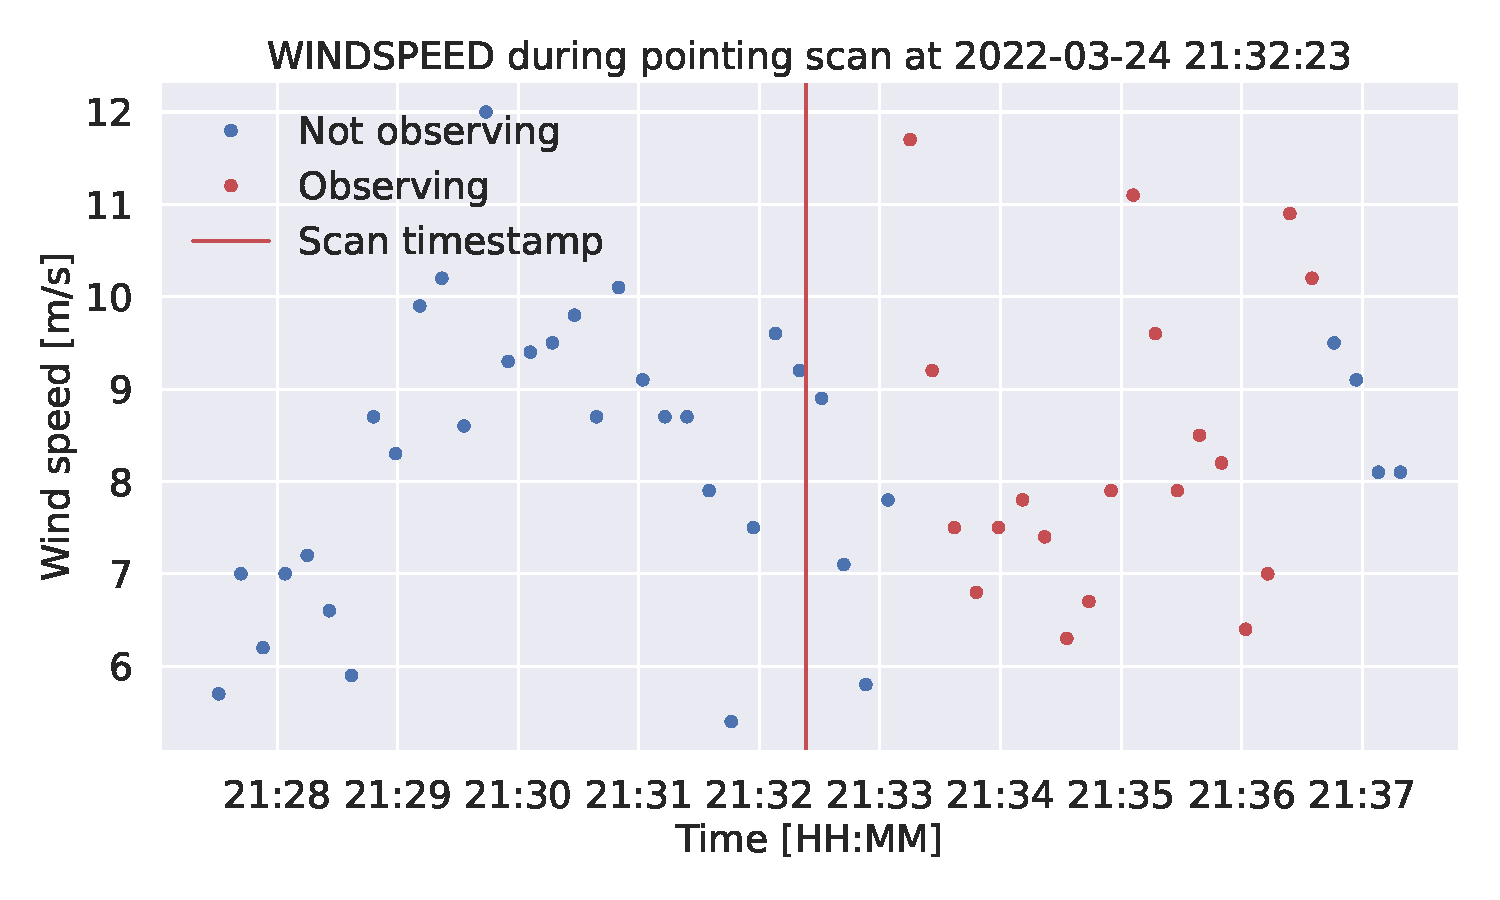
\includegraphics[width=\textwidth]{Feature during scans/scan_WINDSPEED_335.pdf}
        \caption{Wind speed data from the weather station.}
        \label{subfig:scan_windspeed}
    \end{subfigure}
     \caption[Features during pointing scans]{Scatter plots that show different sensory data from before, during, and after a pointing scan. The red line denotes the timestamp for a scan in the pointing scan database.
     The red dots indicate when the telescope is observing, while the blue dots indicate when the telescope is idle or preparing to observe.}
     \label{fig:features_during_scans}
\end{figure}




\subsection{Raw Data}
The raw data from the pointing scans using the NFLASH230 receiver provides input and actual coordinates.
APEX staff has obtained the actual coordinates of the sources by combining the input coordinates with the adjustments made by the pointing model,
automatic adjustments based on sensory data, and the observed offset.
Then, they use this raw data to refine the model fit on data obtained from the optical receiver.
Specifically, this data refines the model of the NFLASH230 model.
Table \ref{tab:raw_datanflash230} is included to provide an example of this data format. 


\begin{table}[h]
    \centering
    \caption[Raw NFLASH230 data]{Extract of raw data obtained with NFLASH230. The data file also includes the source, which is irrelevant to this project.}
    \begin{tabular}{ccccc}
        \toprule
         & \multicolumn{2}{c}{Input} & \multicolumn{2}{c}{Observed} \\ 
        \cline{2-3} \cline{4-5}
        Date & Azimuth & Elevation & Azimuth & Elevation \\ 
        \hline
        2022-01-03 14:24:04 & $189.812879$ & $41.0762$ & $190.254779$ & $40.883651$ \\
        2022-01-03 18:59:40 & $50.842145$ & $73.371647$ & $51.269044$ & $73.203243$ \\
        2022-01-03 19:01:49 & $49.555916$ & $73.752182$ & $49.983112$ & $73.583545$ \\
        2022-01-03 19:16:10 & $39.378382$ & $76.076236$ & $39.781084$ & $75.908956$ \\
        2022-01-03 19:18:27 & $113.934309$ & $39.345667$ & $114.391232$ & $39.170168$ \\
        2022-01-22 13:54:31 & $94.04365$ & $18.148405$ & $94.492505$ & $17.981161$ \\
        2022-01-22 14:15:35 & $148.569964$ & $89.044036$ & $147.783271$ & $88.852306$ \\
        2022-01-22 14:18:15 & $215.664924$ & $49.563821$ & $216.104389$ & $49.386438$ \\
        \bottomrule
    \end{tabular}
    \label{tab:raw_datanflash230}
    \end{table}




\subsection{Tiltmeter Dump Files}
The tiltmeter dump files are a small part of the database and are only used to analyze when pointing scans start and end, using a "scan flag".
In the pointing scan database, there is a timestamp linked to each pointing scan, but this timestamp does not mark the start of the scan, but rather some time right before it.
The tiltmeter dump files contain a flag indicating whether the telescope is idle, preparing to observe, or observing.
There are 280 of these files, and all have filenames in the format "Tiltmeter\_YYYY-MM-DD.dump," which indicates the data's date.
These files contain seven columns: datetime, azimuth, elevation, tilt1x, tilt1y, tilt1t, and the scan flag.
For our purpose, only the datetime and scan flags provide useful information.
Table \ref{tab:tiltmeter_example} shows an extract of the datetime and scan flag columns from one of the tiltmeter dumps.
Analysis of this data is presented in section \ref{sec:scan_duration_analysis}.


\begin{table}[H]
    \centering
    \caption[Tiltmeter dump file]{Extract from a tiltmeter dump file. It shows the timetamp, and a variable denoting if the telescope is a) idle, b) preparing to observer, or c) observing.}
    \begin{tabular}{cc}
        \toprule
        Datetime & Scan flag \\
        \midrule
        2022-11-13T02:23:37 & IDLE \\
        2022-11-13T02:23:38 & IDLE \\
        2022-11-13T02:23:39 & PREPARING \\
        2022-11-13T02:23:40 & PREPARING \\
        $\vdots$ & $\vdots$ \\ 
        2022-11-13T02:23:52 & PREPARING \\
        2022-11-13T02:23:53 & PREPARING \\
        2022-11-13T02:23:55 & OBSERVING \\
        2022-11-13T02:23:56 & OBSERVING \\
        2022-11-13T02:23:57 & OBSERVING \\
        \bottomrule
    \end{tabular}
    \label{tab:tiltmeter_example}
\end{table}


\chapter{Machine Learning Theory}
\section{Supervised learning} \label{sec:supervised_learning}
Supervised learning is a subfield of machine learning that refers to training a model to predict a specific target value based on input data.
In this context, we refer to the input data as "features." The training is supervised when paired with the corresponding target value for prediction.
There are two types of supervised learning, regression and classification. 
In regression, we predict a continuous variable, while in classification predict a binary value, true or false.
The model architecture of the model can be the same regardless of predicting a true/false or continuous value. 
The difference is in the loss function, which is used to evaluate the model's performance during training. The last layer activation function for neural networks is different for regression and classification. 
In-depth explanations of this will come in the following sections.

\section{Loss/Cost} \label{sec:loss_cost}
In machine learning, the loss of a model refers to the discrepancy between the predicted and true values.
It is calculated using a specific function designed to penalize incorrect predictions and measure the model's performance.
The ultimate goal of any machine learning model is to minimize the loss and thereby reduce the difference between predicted and desired outputs.
To achieve this, the model is trained by calculating the gradient of the loss function with respect to different components in the model.
These gradients determine how the model is adjusted to minimize the loss through an iterative process.
As a result, the model is optimized to make better predictions and achieve higher accuracy.\\

The most common loss function for regression is the mean squared error
\begin{equation} \label{eq:mse}
    \mathcal{L}(y, \Tilde{y}) = \frac{1}{N}\sum_{i=1}^N(y-\Tilde{y})^2,
\end{equation}
where $\tilde{y}$ is the prediction, $y$ the true value, and $N$ the number of predictions.

\subsection{Loss Functions}
Loss functions are used to evaluate the performance of the machine learning model during training.
We consider two different loss functions when predicting azimuth and elevation simultaneously with the same model, such as a neural network.
One loss function considers the offset in azimuth and elevation separately, and one considers the total distance.
Let $\Tilde{y}_{Az}$ and $\Tilde{y}_{El}$ denote the prediction for the offset in azimuth and elevation, respectively.
$y_{Az}$ and $y_{El}$ are the true values.
The first loss function is the mean squared error 
\begin{equation}\label{eq:mse1}
    \mathcal{L}_{\text{MSE}} = \frac{1}{2N}\sum_i^N \left( (y_{Az,i}-\Tilde{y}_{Az,i})^2 + (y_{El,i}-\Tilde{y}_{El,i})^2 \right),
\end{equation}
where $N$ is the number of predictions. 
\\
For the second loss function, we use the mean squared distance
\begin{equation}\label{eq:totaloff}
    \mathcal{L}_{\text{MSD}} = \frac{1}{N}\sum_i^N \left[ (y_{Az,i}-\Tilde{y}_{Az,i})^2 + (y_{El,i}-\Tilde{y}_{El,i})^2 \right],
\end{equation}
It is difficult to predict the effects of these loss functions if any at all, but one difference could be that $\mathcal{L}_{\text{MSE}}$ is more sensitive to outliers,
and $\mathcal{L}_{\text{MSD}}$ reduces the offsets more evenly. \\

For models with a single output azimuth or elevation, we use the regular mean squared error \eqref{eq:mse}

\section{Train/test set}
Machine learning models can be highly complex and fit all the data points in a dataset.
While this can result in perfect predictions on the training data, it often leads to poor performance on new data, a phenomenon known as overfitting.
To counteract this, the data is typically split into two parts - a training set and a validation set.
The model is trained on the training set, and the error on the validation set is used to evaluate the model's performance. 
By using a separate set of data for validation, we can better estimate the model's performance on new data and avoid overfitting.

When the error on the training data is low, the model has low bias.
However, if the model is too complex, it may also have high variance, meaning that it is overly sensitive to the training data and unable to generalize well to new data.
A model with high variance may perform well on the training data, but its performance on new data may be poor.
The key to building a good model is to balance bias and variance and to find the right level of complexity that will allow the model to generalize well.
Proper selection of the train/test split ratio and other techniques, such as regularization, can help achieve this balance and improve the model's performance.

One usually picks the machine learning model with the best performance on the validation set, but this performance is not a reasonable estimate of the expected performance on future predictions.
That is because many models are usually trained, and the model with the best performance on the validation set could have gotten lucky.
Therefore, a third test set is used to get an unbiased estimate of the model's performance.
The data in the test set is not used when training or validating and is only used to estimate the final model's performance.


\section{Scaling}
In machine learning, some models, such as neural networks, are highly sensitive to the scale of input data.
The inputs to a model often contain different types of data with varying scales.
Neural networks use weights to transform the input data, and each neuron in a fully connected network receives data from every input feature.
If the input features have different scales, training the weights can be slow and unstable.
Scaling the input data to have the same scale improves the speed and performance of the model.
In contrast, tree-based models are not affected by the range scale of the data since they consist of tests and not mathematical operations.

The most common scaling method is to standardize the data to have zero mean and a standard deviation of one. This is achieved by subtracting the mean and dividing by the standard deviation.
Mathematically, the standardization of a feature $x$ is represented as:

\begin{equation}
x_{scaled} = \frac{x - \mu}{\sigma}
\end{equation}

where $\mu$ is the mean of the feature values, and $\sigma$ is the standard deviation of the feature values.
The mean and standard deviation are computed using the following equations:

\begin{align}
\mu &= \frac{1}{n}\sum_{i=1}^{n}x_i\\
\sigma &= \sqrt{\frac{1}{n}\sum_{i=1}^{n}(x_i - \mu)^2},
\end{align}
where $n$ is the number of observations of the feature.
In addition to standardization, other scaling methods, such as min-max and robust scaling, are also used in specific cases.
Overall, scaling is a crucial step in preprocessing data for machine learning, as it can significantly impact the performance of a model.
However, for tree-based methods, scaling has no effect, as predictions are made based on conditions in the data, not mathematical operations.


\section{Decision Trees}
Decision trees are tree-like models that make decisions based on conditions.
As shown in Figure \ref{fig:decitiontree}, each circle represents a node with various types, including decision nodes that split into two other nodes and leaf/terminal nodes that do not.
The root node is the topmost decision node.
Given an observation, a single path to a leaf node represents the prediction made by the decision tree.

Trees are constructed greedily from the top, meaning that each split is made to minimize the loss function at the current step without considering future splits.
More than a single decision tree is required for complex problems.
Various methods exist to improve decision tree models, as Figure \ref{fig:evolution_of_xgb} demonstrates.
The final step in the figure is XGBoost (Extreme Gradient Boost), a highly efficient and high-performing machine learning algorithm.
This section will briefly cover the methods used to optimize decision trees for prediction.
\cite{Mehta_2019}


\paragraph{Bagging}
Bagging, also known as Bootstrap Aggregation, is a method for training an ensemble of models that contribute to the final prediction.
Each model is trained using bootstrapped data (resampled from the original dataset with replacement), resulting in diverse decision trees.
The final prediction is the average of all ensemble models.

\paragraph{Random Forest}
Random forest is based on bagging, where each tree in the ensemble is made using only a randomly chosen subset of features.
This often leads to better generalization and reduced overfitting.

\paragraph{Boosting}
In boosting, an ensemble is created, but the trees are not made independently.
They are trained one by one, considering the previous trees.
A sample weight is assigned to each sample used to train a tree based on the current ensemble's accuracy.
Samples with significant prediction errors are assigned larger weights, and those with accurate predictions are assigned lower weights.
The final prediction is a weighted sum of all ensemble predictions, with weights based on each tree's accuracy.

\paragraph{Gradient Boosting}
Like in regular boosting, an ensemble of trees is created iteratively by considering the errors made by previous trees.
The process starts with a constant model that predicts the mean of all samples.
The gradient of the loss function with respect to each sample is calculated, and a tree is made to predict these gradients.
The new prediction is the constant plus a small step in the direction of the predicted gradients.
Repeated iteration with small steps in the gradient direction helps reduce both bias and variance.




\begin{figure}[H]
    \centering
    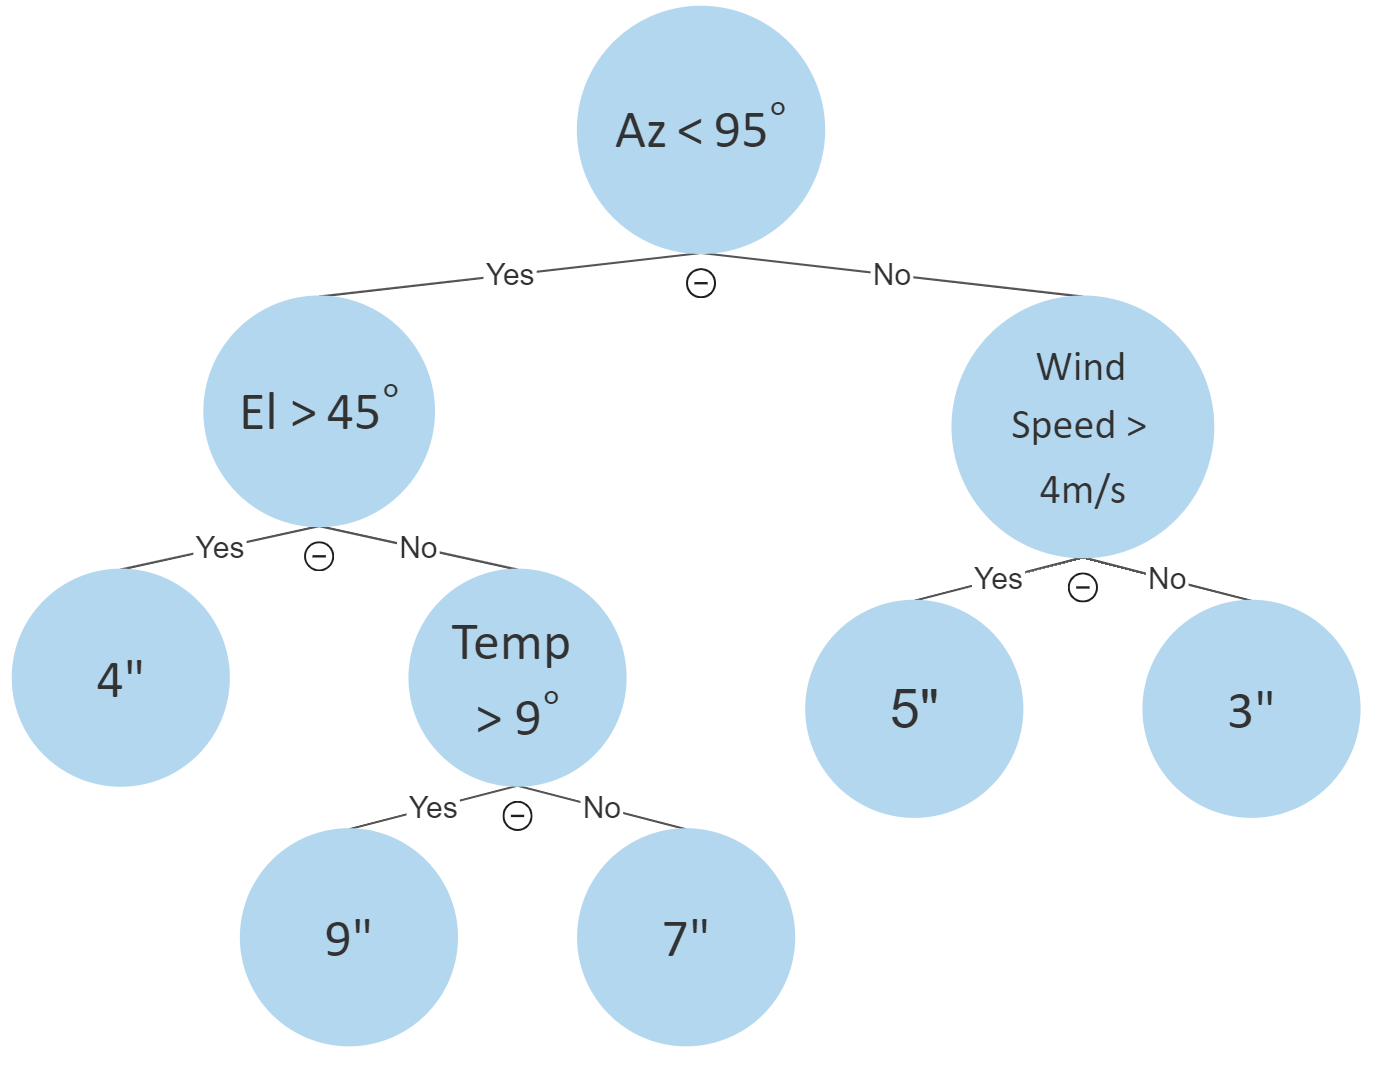
\includegraphics[width=0.98\textwidth]{Other figures/decisiontree_example.PNG}
    \caption{Decision tree with 3 decision nodes and 5 leaf nodes.}
    \label{fig:decitiontree}
\end{figure}

\begin{figure}[H]
    \centering
    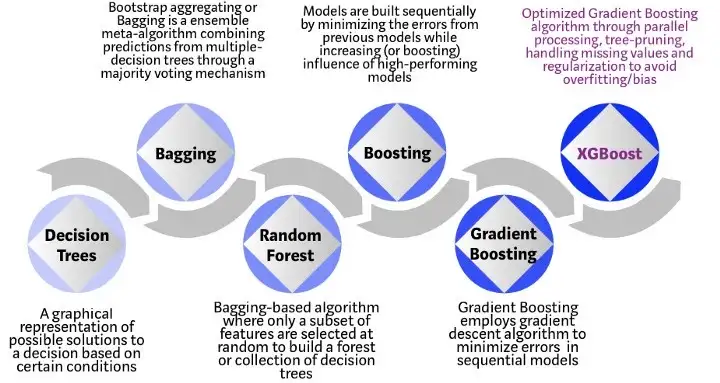
\includegraphics[width=0.98\textwidth]{Other figures/evolution_of_xgb.png}
    \caption{Evolution of XGBoost.
\cite{morde_vishal_nodate}}
    \label{fig:evolution_of_xgb}
\end{figure}

\section{Neural Networks}
A Neural Network (NN) is an Artificial Intelligence (AI) model composed of interconnected neurons inspired by biological neural networks in animal brains.
These networks are arranged in layers, as shown in Figure \ref{fig:nnfig}, and consist of an input layer, one or more hidden layers, and an output layer.
The size of the hidden layer(s) varies depending on the nature of the problem.
A neural network processes input to produce an output, ideally close to the true value.

Each connection in an NN has a trainable weight $w_{jk}^l$, representing the weight from the $k^{th}$ neuron in layer $(l-1)$ to the $j^{th}$ neuron in layer $l$.
Each neuron also has its own bias $b_j$, added to its output to prevent the input to its activation function $\sigma$ from being zero.
The activation function $\sigma$ applied to the neuron's output is the final transformation before passing data to the next layer.
This nonlinear function is crucial in allowing NNs to learn nonlinear relationships in data \cite{universal_approximation}.

The following is the mathematical explanation of how a neuron processes the outputs from the previous layer.

\begin{equation} \label{eq:act_neuron}
    a_{j}^l = \sigma\left(\sum_k w_{jk}^l a^{l-1}_k+b_j^l \right) = \sigma(z_j^l)
\end{equation}
The quantity 
\begin{equation}\label{eq:z_neuron}
    z_j^l = \sum_{k} w_{jk}^l a^{l-1}_k+b_j^l
\end{equation}
will be helpful when explaining how to optimize a neural network and can be considered the weighted input for neuron $j$ in layer $l$.


\begin{figure}[H]
    \centering
    % NEURAL NETWORK activation
% https://www.youtube.com/watch?v=aircAruvnKk&list=PLZHQObOWTQDNU6R1_67000Dx_ZCJB-3pi&index=1
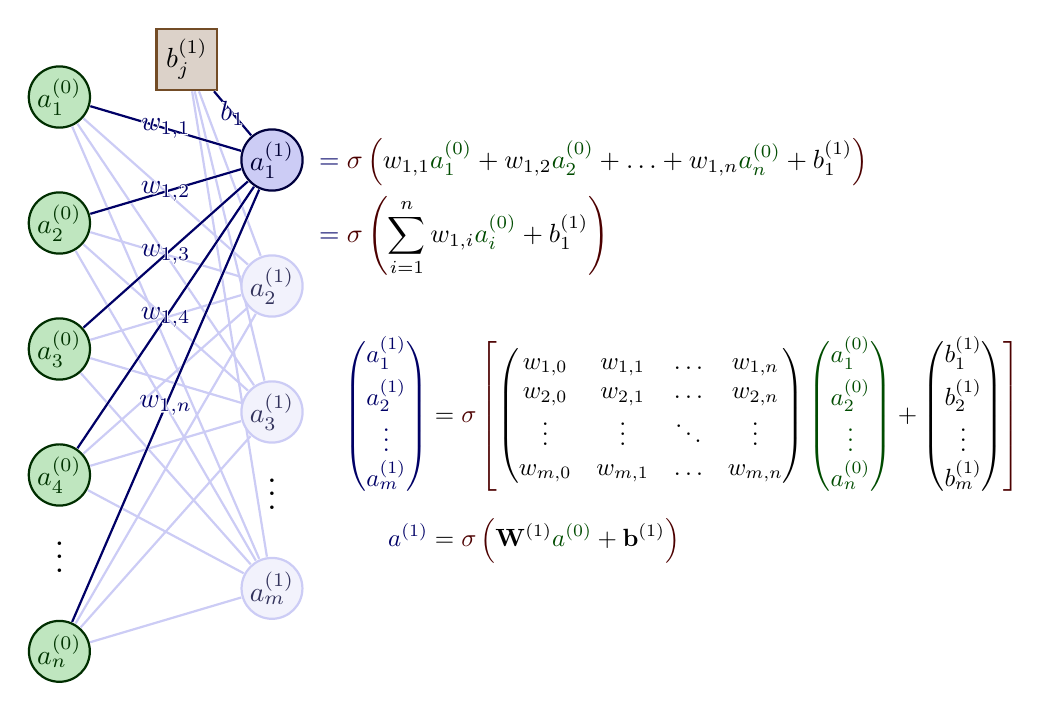
\begin{tikzpicture}[x=2.7cm,y=1.6cm]
  \message{^^JNeural network activation}
  \def\NI{5} % number of nodes in input layers
  \def\NO{4} % number of nodes in output layers
  \def\yshift{0.4} % shift last node for dots
  
  % INPUT LAYER
  \foreach \i [evaluate={\c=int(\i==\NI); \y=\NI/2-\i-\c*\yshift; \index=(\i<\NI?int(\i):"n");}]
              in {1,...,\NI}{ % loop over nodes
    \node[node in,outer sep=0.6] (NI-\i) at (0,\y) {$a_{\index}^{(0)}$};
  }
  
 

  % OUTPUT LAYER
  \foreach \i [evaluate={\c=int(\i==\NO); \y=\NO/2-\i-\c*\yshift; \index=(\i<\NO?int(\i):"m");}]
    in {\NO,...,1}{ % loop over nodes
    \ifnum\i=1 % high-lighted node
      \node[node hidden]
        (NO-\i) at (1,\y) {$a_{\index}^{(1)}$};
      \foreach \j [evaluate={\index=(\j<\NI?int(\j):"n");}] in {1,...,\NI}{ % loop over nodes in previous layer
        \draw[connect,white,line width=1.2] (NI-\j) -- (NO-\i);
        \draw[connect] (NI-\j) -- (NO-\i)
          node[pos=0.50] {\contour{white}{$w_{1,\index}$}};
      }
    \else % other light-colored nodes
      \node[node,blue!20!black!80,draw=myblue!20,fill=myblue!5]
        (NO-\i) at (1,\y) {$a_{\index}^{(1)}$};
      \foreach \j in {1,...,\NI}{ % loop over nodes in previous layer
        %\draw[connect,white,line width=1.2] (NI-\j) -- (NO-\i);
        \draw[connect,myblue!20] (NI-\j) -- (NO-\i);
      }
    \fi
  }

  %\node[node] (b1) at (0.8, 1.5) {$b_1$};
  \node[bias] (B) at (0.6,1.8) {$b_j^{(1)}$}; 
  \draw[connect,white,line width=1.2] (B) -- (NO-1);
  \draw[connect] (B) -- (NO-1) node[pos=0.50] {\contour{white}{$b_1$}};

  % INPUT LAYER
  \foreach \i in {2,...,\NO}{ % loop over nodes
    \draw[connect, myblue!20, on layer=back] (B) -- (NO-\i);
    }


  % DOTS
  \path (NI-\NI) --++ (0,1+\yshift) node[midway,scale=1.2] {$\vdots$};
  \path (NO-\NO) --++ (0,1+\yshift) node[midway,scale=1.2] {$\vdots$};
  
  % EQUATIONS
  \def\agr#1{{\color{mydarkgreen}a_{#1}^{(0)}}}
  \node[below=17,right=11,mydarkblue,scale=0.95] at (NO-1)
    {$\begin{aligned} %\underset{\text{bias}}{b_1}
       &= \color{mydarkred}\sigma\left( \color{black}
            w_{1,1}\agr{1} + w_{1,2}\agr{2} + \ldots + w_{1,n}\agr{n} + b_1^{(1)}
          \color{mydarkred}\right)\\
       &= \color{mydarkred}\sigma\left( \color{black}
            \sum_{i=1}^{n} w_{1,i}\agr{i} + b_1^{(1)}
           \color{mydarkred}\right)
     \end{aligned}$};
  \node[right,scale=0.9] at (1.3,-1.3)
    {$\begin{aligned}
      {\color{mydarkblue}
      \begin{pmatrix}
        a_{1}^{(1)} \\[0.3em]
        a_{2}^{(1)} \\
        \vdots \\
        a_{m}^{(1)}
      \end{pmatrix}}
      &=
      \color{mydarkred}\sigma\left[ \color{black}
      \begin{pmatrix}
        w_{1,0} & w_{1,1} & \ldots & w_{1,n} \\
        w_{2,0} & w_{2,1} & \ldots & w_{2,n} \\
        \vdots  & \vdots  & \ddots & \vdots  \\
        w_{m,0} & w_{m,1} & \ldots & w_{m,n}
      \end{pmatrix}
      {\color{mydarkgreen}
      \begin{pmatrix}
        a_{1}^{(0)} \\[0.3em]
        a_{2}^{(0)} \\
        \vdots \\
        a_{n}^{(0)}
      \end{pmatrix}}
      +
      \begin{pmatrix}
        b_{1}^{(1)} \\[0.3em]
        b_{2}^{(1)} \\
        \vdots \\
        b_{m}^{(1)}
      \end{pmatrix}
      \color{mydarkred}\right]\\[0.5em]
      {\color{mydarkblue}a^{(1)}}
      &= \color{mydarkred}\sigma\left( \color{black}
           \mathbf{W}^{(1)} {\color{mydarkgreen}a^{(0)}}+\mathbf{b}^{(1)}
         \color{mydarkred}\right)
         %\color{black},\quad \mathbf{W}^{(0)} \in \mathbb{R}^{m\times n}
    \end{aligned}$};
  
\end{tikzpicture}
    \caption{This is an illustration of how information is passed through and processed in a neural network.
Generated using TikZ \cite{tikz}}
    \label{fig:nnfig}
\end{figure}




\subsection{Backpropagation}
Backpropagation\cite{backprop_original} is a fundamental algorithm in training artificial neural networks.
It calculates the gradient of the loss function with respect to all the weights and biases in the network,
allowing for updating these parameters to reduce the loss.
The algorithm is based on four key equations, which we describe in this section.\\

We define the error in the $j^\text{th}$ neuron in the $l^\text{th}$ layer by
\begin{equation}\label{eq:bp1} 
    \delta_j^l = \frac{\partial C}{\partial z_j^l} = \frac{\partial C}{\partial a_j^l} \sigma '(z_j^l)
\end{equation}

This can also be considered the partial derivative of the cost function with respect to the bias in neuron $j$ in layer $l$, as 

\begin{equation}\label{eq:bp2}
    \delta_j^l = \frac{\partial C}{\partial z_j^l} = \frac{\partial C}{\partial b_j^l} \frac{\partial b_j^l }{\partial z_j^l} = \frac{\partial C}{\partial b_j^l},
\end{equation}
where we have used the relation $\partial b_j^l / \partial z_j^l = 1$ from rearranging equation \eqref{eq:z_neuron}.
The next equation relates the error in a neuron with the errors in the neurons in the subsequent layer.
\begin{equation}\label{eq:bp3}
    \delta_j^l = \frac{\partial C}{\partial z_j^l} = \sum_k \frac{\partial C}{\partial z_k^{l+1}} \frac{\partial z_k^{l+1}}{\partial z_j^l} = \sum_k \delta_k^{l+1} \frac{\partial z_k^{l+1}}{\partial z_j^l} = \left( \sum_k \delta_k^{l+1} w_{kj}^{l+1} \right) \sigma '(z_j^l)
\end{equation}
Note that the indices on the weight $w$ are now swapped.
We may think of this equation as an error propagating backward by multiplying the error in layer $l+1$ with the transpose of the weight connecting layer $l$ with $l+1$
We derive the final equation from the partial derivative of the cost function with respect to the weight $w_{jk}^l$
\begin{equation}\label{eq:bp4}
    \frac{\partial C}{\partial w_{jk}^l} = \frac{\partial C}{\partial z_j^l} \frac{\partial z_j^l}{\partial w_{jk}^l} = \delta_j^l a_k^{l-1}
\end{equation}

Equation \eqref{eq:bp1} lets us calculate the error in the last layer, and using equation \eqref{eq:bp3}, we can propagate this error backward through the network, calculating the error for all the neurons.
We then use equations \eqref{eq:bp2} and \eqref{eq:bp4} to calculate the gradient of the cost function with respect to the weights and biases.


\subsection{Gradient Descent}
Gradient Descent (GD) is an iterative optimization algorithm used in machine learning for minimizing a differentiable function.
The goal of GD is to update the model's trainable parameters in such a way that the loss function is minimized.
In mathematical terms, we aim to find the values of the parameters $\boldsymbol{\theta}$ that minimize the objective function $\mathcal{L}(\bold{x}, \boldsymbol{\theta})$, where $\bold{x}$ represents the input data.
The loss function is typically defined as the mean squared error \eqref{eq:mse} for regression problems, so
\begin{equation}
    \mathcal{L}(\bold{x}, \boldsymbol{\theta}) = \frac{1}{N}\sum_{i=1}^N(y_i-f(\bold{x}_i, \boldsymbol{\theta}))^2,
\end{equation}
where $f(\bold{x}_i, \boldsymbol{\theta})$ is the output of the model for input data $\bold{x}_i$, and $y_i$ is the target value.

To achieve the goal, GD involves calculating the gradient of the loss function with respect to the model's trainable parameters and updating them iteratively by taking a small step in the negative direction of the gradient.
The iterative update rule can be expressed as follows:

\begin{align}
\bold{v}_t &= \eta_t \nabla_\theta \mathcal{L}(\bold{x}, \boldsymbol{\theta}), \\
\boldsymbol{\theta}_{t+1} &= \boldsymbol{\theta}_t - \bold{v}_t,
\end{align}

where $\eta$ denotes the learning rate, and $\nabla_\theta$ denotes the gradient with respect to $\boldsymbol{\theta}$.
The learning rate determines the step size of the update, and it is important to choose a suitable value to ensure convergence of the optimization.

One major limitation of GD is that it can get stuck in local minima, yielding suboptimal results.
The choice of initial parameter values $\boldsymbol{\theta}$ can also impact the final optimized model.
Moreover, computing the gradient using the entire dataset can be computationally expensive for large datasets.
To address these limitations, various modifications of GD have been proposed,
such as stochastic gradient descent (SGD) and mini-batch gradient descent (MBGD),
which compute the gradient using only a subset of the data at each iteration.
These modifications can help to accelerate the convergence and improve the scalability of GD.

\subsection{Stochastic Gradient Descent}
Stochastic Gradient Descent (SGD) is a widely used optimization algorithm in machine learning that addresses some of the limitations of Gradient Descent (GD).
Unlike GD, which computes the gradient using the entire dataset at each iteration, SGD computes the gradient using only a randomly sampled subset, called a mini-batch.
This makes SGD more efficient and less computationally expensive than GD, particularly for large datasets.
Furthermore, by randomly sampling mini-batches, SGD is more likely to escape local minima and converge to the global minimum.
The update rule for SGD can be derived similarly to that for GD, with the only difference being the replacement of the full dataset with a mini-batch.
By iteratively updating the model's parameters using mini-batches, SGD can converge faster and more robustly than GD.

However, SGD also has limitations to consider. If the learning rate is too large, the optimization may overshoot the minimum and fail to converge.
On the other hand, if the learning rate is too small, the optimization may converge very slowly.
In addition, if there are areas in the function space with small gradients, the optimization may stagnate and fail to converge.
To address these limitations, various modifications of SGD have been proposed, such as adaptive learning rate methods like Adagrad and RMSprop,
which adjusts the learning rate dynamically based on the history of the gradients.
These modifications can improve the stability and convergence speed of SGD.


\subsection{Momentum GPT}

In practice, SGD is mostly used with momentum.
Momentum serves as a memory of previous momenta and can improve the convergence speed of SGD, particularly in areas of the function space with low gradients, such as local minima.

The update rule for momentum can be expressed as follows:
\begin{align}
\bold{v}_t &= \gamma \bold{v}_{t-1} + \eta_t \nabla_\theta \mathcal{L}(\bold{x}, \boldsymbol{\theta}) \\
\boldsymbol{\theta}_{t+1} &= \boldsymbol{\theta}_t - \bold{v}_t,
\end{align}
where $\gamma$ is the momentum parameter with $0 \leq \gamma \leq 1$.
The momentum term considers the update of the previous step, in addition to the gradients at the current step.
By incorporating previous momenta, momentum can smooth out variations in the optimization trajectory and accelerate convergence towards the minimum.

Momentum is particularly useful when the gradient direction is consistent across many iterations, as it allows the optimization to maintain a higher velocity in the same direction.
In contrast, in areas of high variance or noisy gradients, momentum may cause overshooting and slow down convergence.
To address this, adaptive momentum methods like Adam have been proposed, which adjust the momentum parameter dynamically based on the history of the gradients.
These methods can improve the convergence speed and stability of momentum-based optimization algorithms.


\subsection{Adam GPT}
Adam is an optimization algorithm that combines the benefits of both SGD with momentum and adaptive learning rate methods.
It uses a running average of the first and second moments of the gradient to compute per-parameter adaptive learning rates.
Adam updates the parameters iteratively as follows:

\begin{align}
\bold{g}_t &= \nabla_\theta \mathcal{L}(\bold{x}, \boldsymbol{\theta}) \\
\bold{m}_t &= \beta_1 \bold{m}{t-1} + (1-\beta_1) \bold{g}_t \\
\bold{s}_t &= \beta_2 \bold{s}{t-1} + (1-\beta_2) \bold{g}_t^2\\
\hat{\bold{m}}_t &= \frac{\bold{m}_t}{1 - (\beta_1)^t} \\
\hat{\bold{s}}_t &= \frac{\bold{s}_t}{1 - (\beta_2)^t} \\
\boldsymbol{\theta}_{t+1} &= \boldsymbol{\theta}_t - \eta_t \frac{\hat{\bold{m}}_t}{\sqrt{\hat{s}_t} + \epsilon},
\end{align}

where $\bold{g}_t$ denotes the gradient at time step $t$, $\bold{m}_t$ and $\bold{s}_t$ are the first and second moment estimates, respectively.
$\beta_1$ and $\beta_2$ control the decay rate of the first and second moments, respectively.
$\eta_t$ is the learning rate, and $\epsilon$ is a regularization constant to prevent division by zero.

Adam has several advantages over other optimization algorithms, including its ability to adaptively compute per-parameter learning rates and the robustness of its estimates to noise in the gradient.
The adaptive learning rates can help speed up convergence and lead to better performance.
Furthermore, the memory of previous first and second-order gradient estimates enables the algorithm to be more robust to noise and outliers in the data.
As a result, Adam is widely used and has become the de facto standard optimization algorithm in deep learning.


\subsection{Activation functions}
Activation functions play a crucial role in training a neural network by allowing it to learn non-linear relationships between inputs and outputs.
Different activation functions have varying properties; we will discuss some of the most common ones in this section.
Properties like non-linearity, differentiability, monotonicity, smoothness, and zero-centering are important for activation functions.
Non-linearity enables the model to capture complex relationships, differentiability is necessary for calculating the derivative of the loss function with respect to the trainable weights, monotonicity helps ensure stability in activation outputs, smoothness stabilizes gradients during training, and zero-centering balances the activation distribution within the model.

\begin{itemize}
    \item Non-linearity enables the model to capture complex relationships
    \item Differentiability is necessary for calculating the derivative of the loss function with respect to the trainable weights
    \item Monotonicity helps ensure stability in activation outputs, smoothness stabilizes gradients during training
    \item Smoothness: A smooth activation function helps stabilize the gradients and training.
    \item Zero-centering balances the activation distribution within the model.
\end{itemize}

\paragraph{Tanh}
Tanh, the hyperbolic tangent function is given by
\begin{equation}\label{eq:tanh}
    Tanh(x) = \frac{e^x+e^{-x}}{e^x-e^{-x}}
\end{equation}

\paragraph{ReLU}
The Rectified Linear Unit (ReLU) activation function pushes all negative values to zero while leaving positive values unchanged,
which introduces non-linearity while solving the vanishing gradients problem by having a gradient of either 0 or 1 for negative and positive values, respectively.
\begin{equation}\label{eq:relu}
    ReLU(x) = \begin{cases} x & \mbox{if } x > 0 \\ \mbox{0,} & \mbox{otherwise} \end{cases}
\end{equation}

\paragraph{GeLU}
The Gaussian Error Linear Unit (GeLU) is a smooth approximation of the ReLU function, given by
\begin{equation}
    GeLU(x) = x \Phi (x),
\end{equation}
where $\Phi(x)$ is the standard Gaussian cumulative distribution function.

GeLU can be approximated with
\begin{equation}
    GeLU(x) \approx 0.5x \left( 1+\tanh\left[\sqrt{2/\pi}(x+0.044715x^3)\right] \right),
\end{equation}
which is faster to compute than the original definition but can result in worse performance.
For computational efficiency, we used this approximation.


\section{Model Explainability}
In the context of machine learning, SHAP \cite{SHAP} and SAGE \cite{SAGE} apply the same idea to determine the contribution of each feature to a prediction.
SHAP provides a local explanation by computing the contribution of each feature to the prediction of a single data point.
On the other hand, SAGE provides a global explanation by computing each feature's contribution to the model's overall prediction performance.
These methods allow us to understand the relationship between the features and the prediction, particularly useful when the model is too complex to interpret.
Additionally, they provide a way to validate the model's fairness and bias.
By understanding which features contribute the most to a prediction, one can determine if the model is fair or biased and if the prediction is trustworthy.\\

Both SHAP and SAGE methods are based on Shapley values \cite{shapley_value_1953}, a concept in game theory introduced by Lloyd Shapley in 1951.
Shapley values determine each player's contribution to a group's surplus or overall value.
The explanation below of Shapley values, SHAP, and SAGE is inspired by a blog post by Ian Covert \cite{covert_shap_sage}.\\

The Shapley value for a player $i$ in a cooperative game with $d$ players is

\begin{equation}
    \phi_i(w) = \frac{1}{d} \sum_{S \subseteq D \backslash \{ i \} } \binom{d-1}{|S|}^{-1} \left[ w(S\cup \{ i \} ) - w(S) \right]
\end{equation}

where $D$ is the set of all players, $S$ is a coalition of players, $w(S)$ is the value of the coalition $S$, and $|S|$ is the number of players in the coalition.
This formula satisfies four important conditions:
\begin{itemize}
    \item Efficiency: The sum of all Shapley values is equal to the group's total value.
    \item Symmetry: If two players $i$ and $j$ have the same impact on all coalitions with $w(S \cup \{i\}) = w(S \cup \{j\})$ for all $S$, they should have the same Shapley value $\phi_i(w) = \phi_j(w)$.
    \item Dummy: A player $i$ that makes no contribution to the group with $w(S \cup \{i\}) = w(S)$, should receive a value of zero, or $\phi_i(w)=0$.
    \item Linearity: A player's value is proportional to their contribution to the group.
If player $i$ contributes twice as much as player $j$ to the group's overall worth, then player $i$ should have twice the Shapley value.
\end{itemize}

\subsection{SHAP}
Shapley values explain how each feature $(x^1, \dots, x^d)$ in a model $f$ contributes to the deviation from the mean prediction $\mathbb{E}[f(x)]$ of the dataset for a single prediction.
It assigns a value $\phi_1, \dots, \phi_d$ to each feature that quantifies the feature's influence on the prediction $f(x)$.
SHAP (Shapley Additive Explanations) computes approximate Shapley values for machine learning models.\\

We define a cooperative game $v_{f,x}$ to represent a prediction given the features $x^S$, as
\begin{equation}
    v_{f,x}(S) = \mathbb{E} \left[ f(X) | X^S = x^S \right],
\end{equation}

where $x^S$ are known, and the remaining features are treated as random variable $X^{\Bar{S}}$ (where $\Bar{S} = D \backslash S$).
This is the mean prediction $f(X)$ when the unknown values follow the conditional distribution $X^{\Bar{S}} | X^S = x^S$.\\

Using a subset of features from the prediction while sampling the rest from the dataset reduces the chance of improbable samples.
Given this convention for making predictions, we can apply the Shapley value to define each feature's contribution to the prediction $f(X)$ using Shapley values $\phi_i(v_{f,x})$.
A Shapley value of $\phi_i(v_{f,x}) > 0$ indicates that feature $i$ contributes to an increase in prediction $f(X)$.
A negative Shapley value $\phi_i(v_{f,x}) < 0$ indicates the opposite, that the feature contributes to a decrease in $f(X)$.
Uninformative features will have small values $\phi_i(v_{f,x}) \approx 0$.

\subsection{SAGE}
SAGE (Shapley Additive Global Importance) explains how every feature contributes to the model's overall performance, and it relates to SHAP in a simple way.
For a given feature, the global feature importance is the average SHAP value (for that feature) across all samples in the dataset.
This is, however, different from how it is calculated in practice.
A paper by Ian Covert et al.
\cite{sage_paper} on global feature importance proposes an algorithm that aims directly at a global feature explanation, unlike the SHAP values, which makes
it faster.
This is the algorithm used for approximating the SAGE values for the features in the thesis.

\section{Mutual Information}
Mutual information is a fundamental measure of the statistical dependence between two random variables,
providing a way to quantify the amount of information one variable conveys about the other.
For a pair of discrete random variables $X$ and $Y$, we have 
\begin{equation}
    I(X;Y) = \sum_{y} \sum_{x} p(x,y) \log \left( \frac{p(x,y)}{p(x)p(y)} \right),
\end{equation}
where $p(x,y)$, $p(x)$, and $p(y)$ are the joint and marginal probabilities, respectively.
The mutual information captures linear and nonlinear relationships between variables, unlike Pearson's correlation coefficient, which can only detect linear relationships.
However, mutual information has limitations in that it relies on binning the data, which can introduce bias and limit the resolution of the information.
   
Furthermore, estimating mutual information for high-dimensional data sets can be computationally expensive.
Despite these limitations, mutual information remains a popular tool in feature selection, data visualization, and machine learning.

\part{Data Processing \& Methods}
\chapter{Data Processing}

This chapter of the thesis outlines the methodology used for data analysis, cleaning, transformation, and feature engineering.
Data-driven methods have the potential to learn all relations in the data, but the size of the dataset limits this.
Therefore, cleaning the data and selecting features containing information relevant to the desired output is essential.
With the system's complexity, identifying relevant features can be challenging.
To address this, we employed data-driven modeling to help identify important features while using feature engineering to incorporate
our understanding of the system and create informative features.

Cleaning data involves removing irrelevant data that could confuse the model, thereby ensuring that the model learns from the most relevant information.
Feature engineering involves incorporating domain knowledge into the model to create features that provide additional information.

We performed data analysis to decide which features to train our models.
This analysis involves understanding the relationships between the different variables in the dataset and identifying which variables
could be helpful in predicting the target variable.


\section{Cleaning Pointing Scan Data} \label{sec:cleaning_pt_scan}

When utilizing data-driven modeling for predictive purposes, ensuring that the dataset is clean and informative is crucial.
In this project, various factors may impact the quality of the data, and therefore, we implemented measures to clean the data based on our knowledge of the telescope's operation.
We employed a criteria-based approach and a machine learning classifier to remove pointing scans from the dataset.
During the removal of pointing scans, it is important to strike a balance between removing noise and retaining relevant information.
Outliers in the training data can introduce bias into machine learning models, as these data points may not accurately represent typical conditions.
Consequently, having outliers in the training data can be more damaging than removing good pointing scans.
Therefore, we have a strict approach when cleaning the data to ensure high-quality datasets for model training.


\subsection{Cleaning Criteria}
To eliminate unreliable or unusable scans, we applied criteria informed by the insights of astronomers at APEX.
The following list outlines the criteria used to filter out such scans:
\begin{itemize}
    \item Scans using the HOLO transmitter:
    These scans are aimed at a radio tower and are not realistic data for training an ML model.
    \item Scans using ZEUS2:
    These are highly experimental pointing scans and unreliable.
    \item Scans using CHAMP690: There are very few scans with this instrument.
    \item Scans in January and February of $2022$: The weather is unreliable and there are few scans in this period.
    \item Scans that are tracking tests
    \item Scans after 17.09.2022 since we only have sensory data until this point
\end{itemize}   
After this filtering, there were $5901$ out of $8862$ scans left.
        
\subsection{Pointing Scan Classifier} 
\subsubsection{Method}
In addition to cleaning the data based on the criteria above, we had to remove the outright bad pointing scans (like \ref{subfig:bad_continuous} \ref{subfig:bad_line}, \ref{subfig:bad_line}).
The scan quality is often obvious when inspecting the data visually, but it is hard to develop suitable measures to identify which scans are good or bad.
Instead, we trained a classifier to predict whether a scan is of good or bad quality.
We used an XGBoost classifier with 13 features as inputs, all of which are present in the pointing scan figures (\ref{fig:line_pointings} and \ref{fig:continueous_pointings}).
The first 12 features are the amplitudes, FWHMs, pointing offsets, and these values' uncertainties.
The last feature is the beamwidth of the telescope for the given observing frequency.\\

We had to label a dataset set by manually looking at pointing scans.
The size of the dataset set was $369$ samples with $270$ good and $99$ bad scans.
Table \ref{tab:xgb_hyperparameters_clf} shows the hyperparameters and search ranges we used when optimizing this model, along with the resulting best parameter values.
We also used \textit{scale\_pos\_weight} to consider the unbalanced classes, for which the value is the ratio of negative to positive classes (number of bad scans divided by the number of good scans).
We split the data into $80\%$ for training and the rest for validating, corresponding to $295$ and $74$ samples for training and validation, respectively.

\begin{table}[H]
    \centering
    \caption[Hyperparemter search space XGBoost pointing scan classifier]{This table presents a list of parameters we sampled during hyperparameter tuning for the pointing scan classifier.
    The table includes names, sampled distributions and corresponding ranges, and parameter values for the best model.}
    \begin{tabular}{lccc}
        \toprule
        Parameter & Sample Distribution & Range & Best Parameter Value\\ \hline
        max depth & Uniform & [$1$, $5$] & $2$\\ 
        n estimators & Uniform & [$1$, $80$] & $53$\\ 
        \bottomrule
    \end{tabular}
    \label{tab:xgb_hyperparameters_clf}
\end{table}

\subsubsection{Results}
The XGBoost classifier performed well with a $97\%$ overall accuracy on the validation set.
Figure \ref{fig:pointing_scan_clf} shows the precision-recall curve on the left and the average precision curve on the right.
From the precision-recall curve, it is clear that we can achieve close to $100\%$ precision while still having a high recall.
We select a large threshold such that the classifier removes most bad scans from the training data,
because a bad pointing scan is potentially more harmful for the model than discarding a few good scans.
The average precision curve shows an optimal threshold for maximizing the precision, which is about $80\%$.\\

We used the classifier to clean the dataset further, using prediction threshold $0.8$, we remove another $575$ scans, leaving us with
$5326$ scans for the rest of the analysis.


\begin{figure}[H]
    \centering
    \begin{subfigure}[t]{0.49\textwidth}
        \centering
        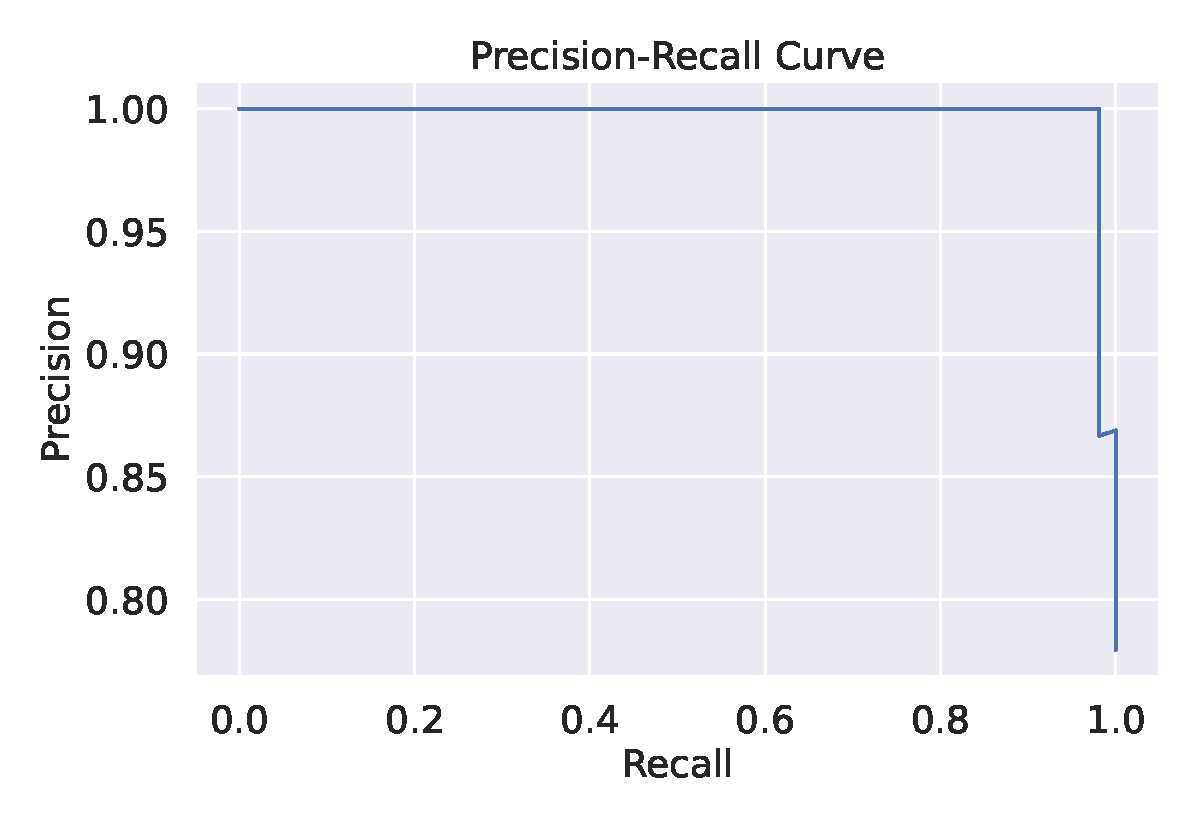
\includegraphics[width=1\textwidth]{Clf/precision_recall_curve_both.pdf}
        \caption{Precision-recall curve on the test set.}
        \label{subfig:pr_curve}
    \end{subfigure}
    \begin{subfigure}[t]{0.49\textwidth}
       \centering
       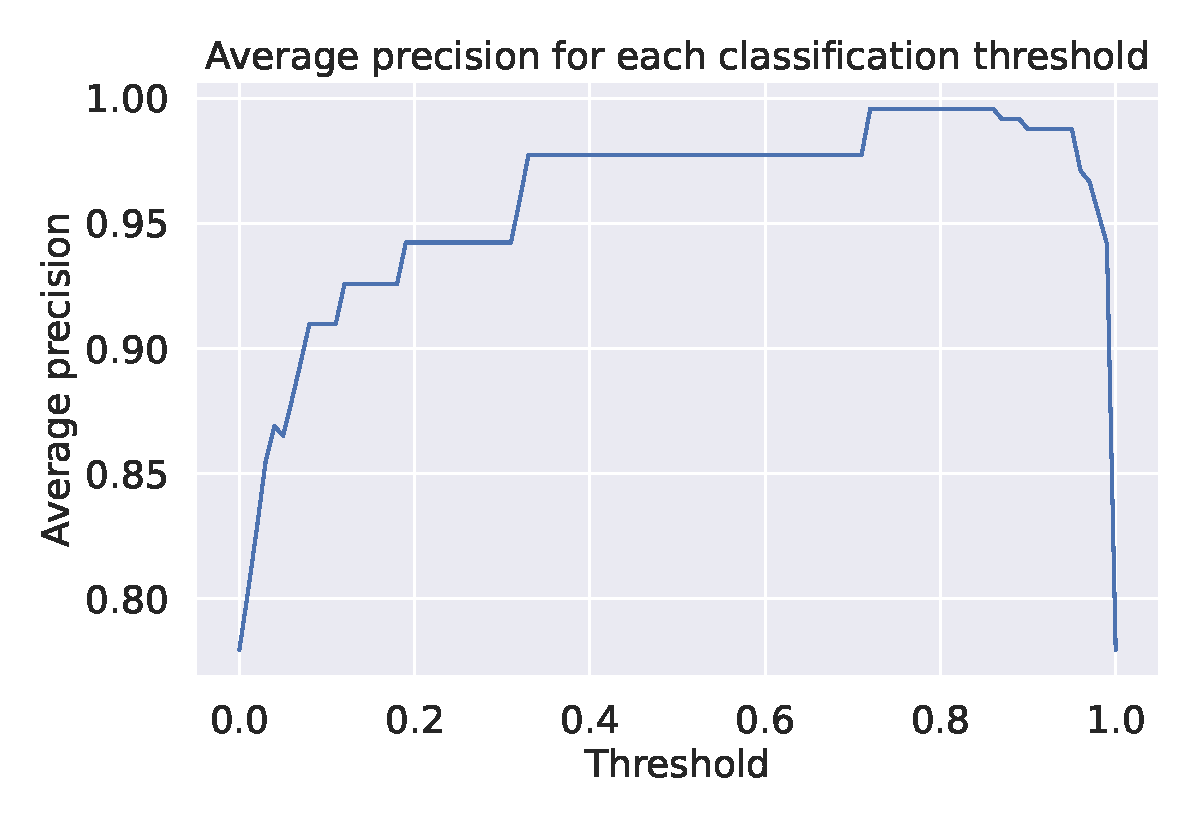
\includegraphics[width=1\textwidth]{Clf/mAP_curve_both.pdf}
       \caption{Average precision for different classification threshold.}
       \label{subfig:map_curve}
    \end{subfigure}
     \caption[Performance plots of XGBoost pointing scan classifier]{Precision-recall and average precision curve for the XGBoost classifier when classifying good and bad pointing scans in the test set.}
     \label{fig:pointing_scan_clf}
\end{figure}



% \\~\\
% \begin{subfigure}[t]{0.49\textwidth}
%     \centering
%     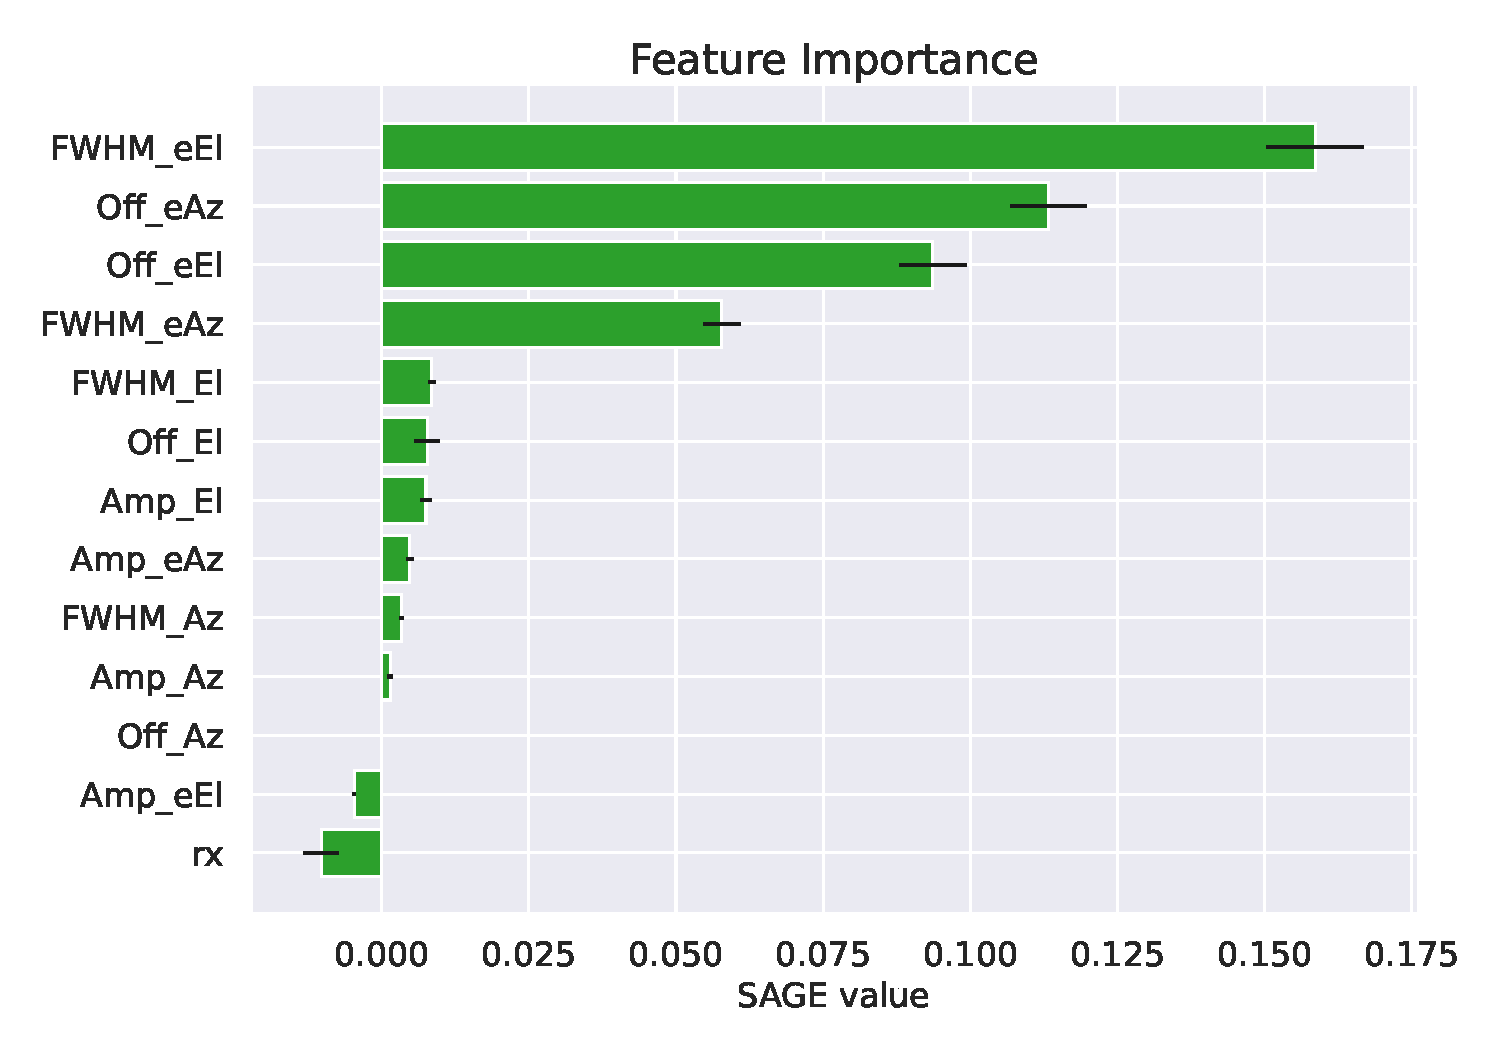
\includegraphics[width=1\textwidth]{Clf/Sage_xgb_clf_rx.pdf}
%     \caption{Average precision for different classification threshold.}
%     \label{subfig:xgb_clf_sage}
% \end{subfigure}
% \begin{figure}[H]
%     \centering
%     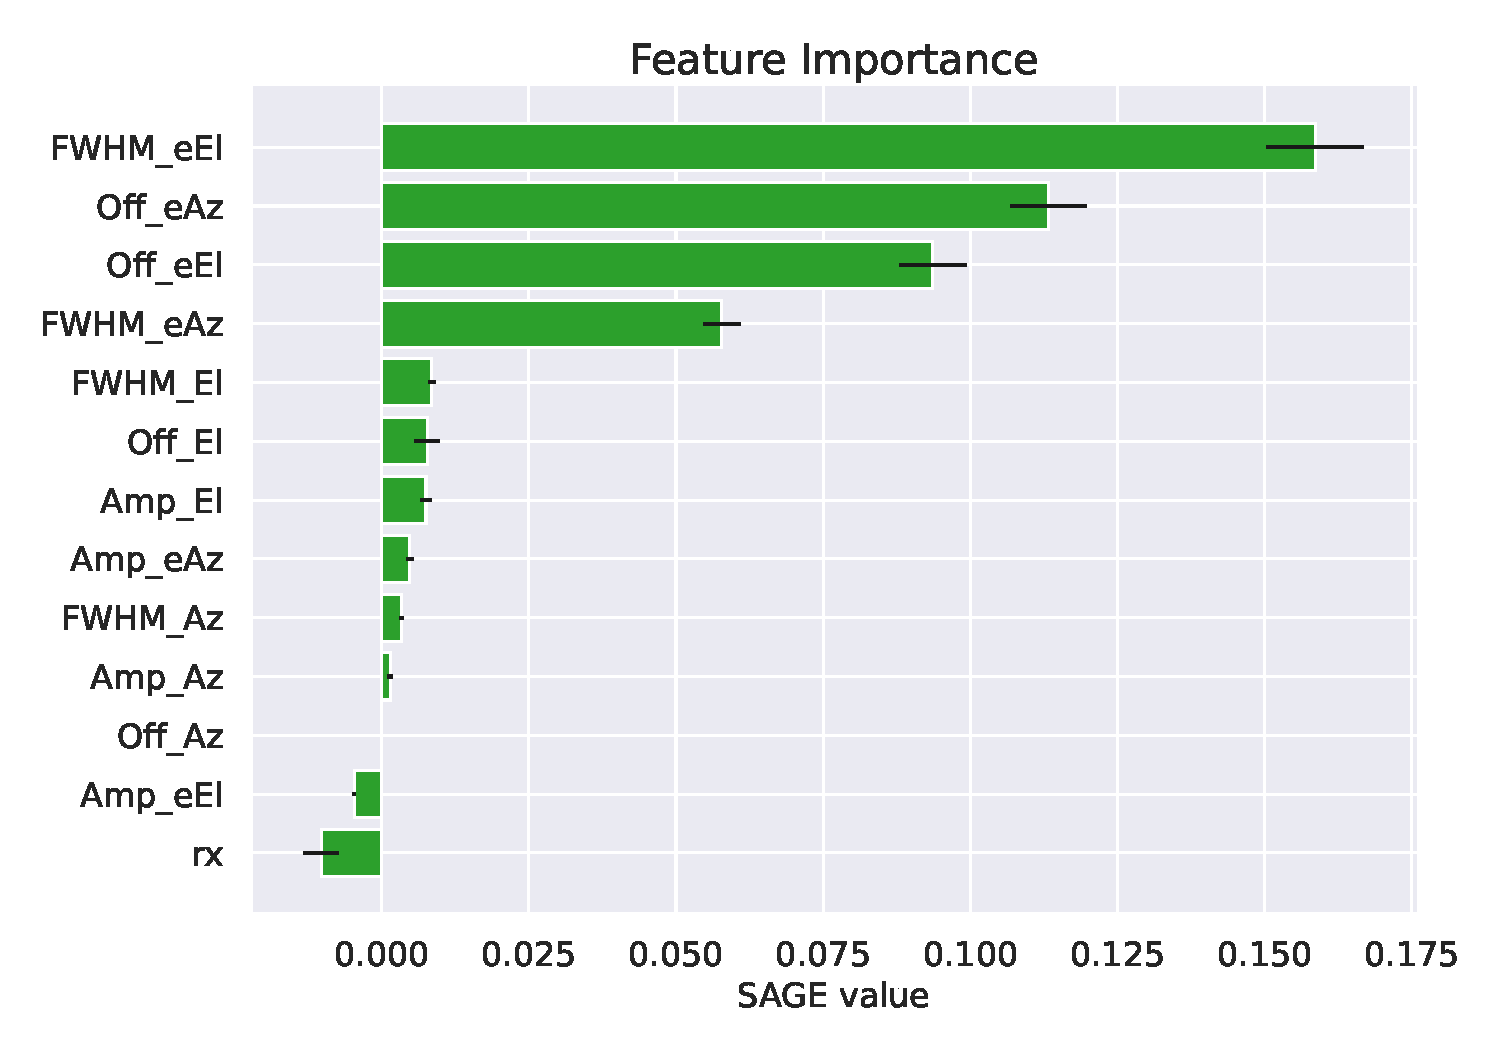
\includegraphics[width=0.98\textwidth]{Clf/Sage_xgb_clf_rx.pdf}
%     \caption{SAGE values for the XGB classifier.}
%     \label{fig:xgb_clf_sage}
% \end{figure}

\section{Scan Duration Analysis}\label{sec:scan_duration_analysis}
As mentioned in the database section \ref{sec:database}, the scans' timestamps are not the accurate start time of a scan.
The tiltmeter dump files with the flag indicating whether the telescope is idle, preparing to observe, or observing,
is the only accurate data we have when the telescope performs a pointing scan.
Therefore, we need to combine the timestamp of the pointing scan with the flag in the dump files to analyze the duration of scans.

\subsection{Analysis}
First, we convert the different scan flags to numbers.
\textit{IDLE} and \textit{PREPARING} is the set $0$, and \textit{OBSERVING} is set to $1$.
Then we can subtract the previous rows from all rows, resulting in the value $1$ when the scan starts, and $-1$ when it ends.
Table \ref{tab:scan_flag_difference} shows an example of the result.


\begin{table}[H]
    \centering
    \begin{tabular}{cccc}
        \toprule
        Time & Flag & Flag Integer & $\Delta$ \\
        \midrule
        11:21:21 & IDLE & $0$ & $0$ \\
        11:21:22 & PREPARING & $0$ & $0$ \\
        11:21:23 & OBSERVING & $1$ & $1$ \\
        11:21:24 & OBSERVING & $1$ & $0$ \\
        11:21:25 & OBSERVING & $1$ & $0$ \\
        11:21:26 & IDLE & $0$ & $-1$ \\
        \bottomrule
    \end{tabular}
    \caption[Tiltmeter dump file with $\Delta$ for analysis]{This table shows the tiltmeter dump file containing the telescope state flag,
            and how we found the start ($\Delta = 1$) and end ($\Delta = -1$) of a scan.}
    \label{tab:scan_flag_difference}
\end{table}


\subsection{Algorithm}
With the scan timestamp and the observing flag from tiltmeter dumps, we used the following algorithm to obtain the start and end of pointing scans.

\begin{algorithm}[H]
    \caption{Algorithm that finds the start and end of pointing scan}
    \label{alg:scan_times}
    \begin{algorithmic}
        \Require{\\
        \begin{itemize}
            \item Pointing scan timestamps $D=\{D_1,\dots,D_n\}$
            \item Timestamps $T=\{T_1,\dots,T_m\}$ and scan flag $F=\{F_1,\dots,F_m\}$
        \end{itemize}}
        \Ensure{Start and end of pointing scans $S=\{S_i,\dots,S_n\}$ and $E=\{E_i,\dots,E_n\}$}
        \For{$i=1,\dots,m$}
            \If {$F_i=OBSERVING$}
                \State {$F_i = 1$}
            \Else
                \State {$F_i = 0$}
            \EndIf
        \EndFor
        \\
        \For{$i=1,\dots,n$}
            \State {$\hat{T} = \{T_j, \text{  if  } T_j > D_i\}_j^m$}
            \State {$\hat{F} = \{F_j, \text{  if  } T_j > D_i\}_j^m$}
            \ForAll {$t_i,f_i \text{ in } \hat{T},\hat{F}$}
                \State {$\Delta = f_i-f_{i-1}$}
                \If {$\Delta = 1$}
                    \State {$S_i = t_i$}
                \EndIf
                \If {$\Delta = -1$}
                    \State {$E_i = t_i$}
                    \State {Continue}
                \EndIf
            \EndFor
        \EndFor
    \end{algorithmic}
\end{algorithm} 


\subsection{Results}
By analyzing start and end timestamps for all the scans we had tiltmeter dumps for,
we see that the first \textit{OBSERVING} flag present after a scan is on average $53.9$ seconds after the scan timestamp on average, with a standard deviation of $20.5$ seconds.
Figure \ref{fig:scan_times_box} shows boxplots of this time difference for each of the instruments, which strongly indicates that assuming the starting point of a scan is $53.9$ seconds after
the timestamp is reasonable.
In the same plot, we also see that the starting time is fairly constant for the different instruments.
The right plot of Figure \ref{fig:scan_times_date} shows the time difference in seconds between the first observing flag after a scan timestamp throughout the year.
From the plot, this stays constant over time.\\

Now that we have found the starting points of the pointing scans, we can look at their duration.
The left plots in Figure \ref{fig:scan_times_date} and \ref{fig:scan_times_box} show the duration of the pointing scans for different instruments.
From these figures, it is clear that the duration of a pointing scan varies a lot.
A varying scan duration is problematic because we only have these tiltmeter dump files for $2875/8381\approx 34\%$ of the pointing scans. 
To address this issue, we collected data for feature engineering over a shorter period of time.
It is important to note that using data from after a pointing scan has ended can be inaccurate, as the telescope may start observing a different source.
When examining the scatter plot of scan durations, we observed clusters of scans around $60$-$70$ seconds, $120$-$130$ seconds, and so on.
To ensure that we collected during a pointing scan, we did not use data from more than $60$ seconds after the start of a scan.
For the scans with an exact start and end time, we used this time period instead. 


\begin{figure}[H]
    \centering
    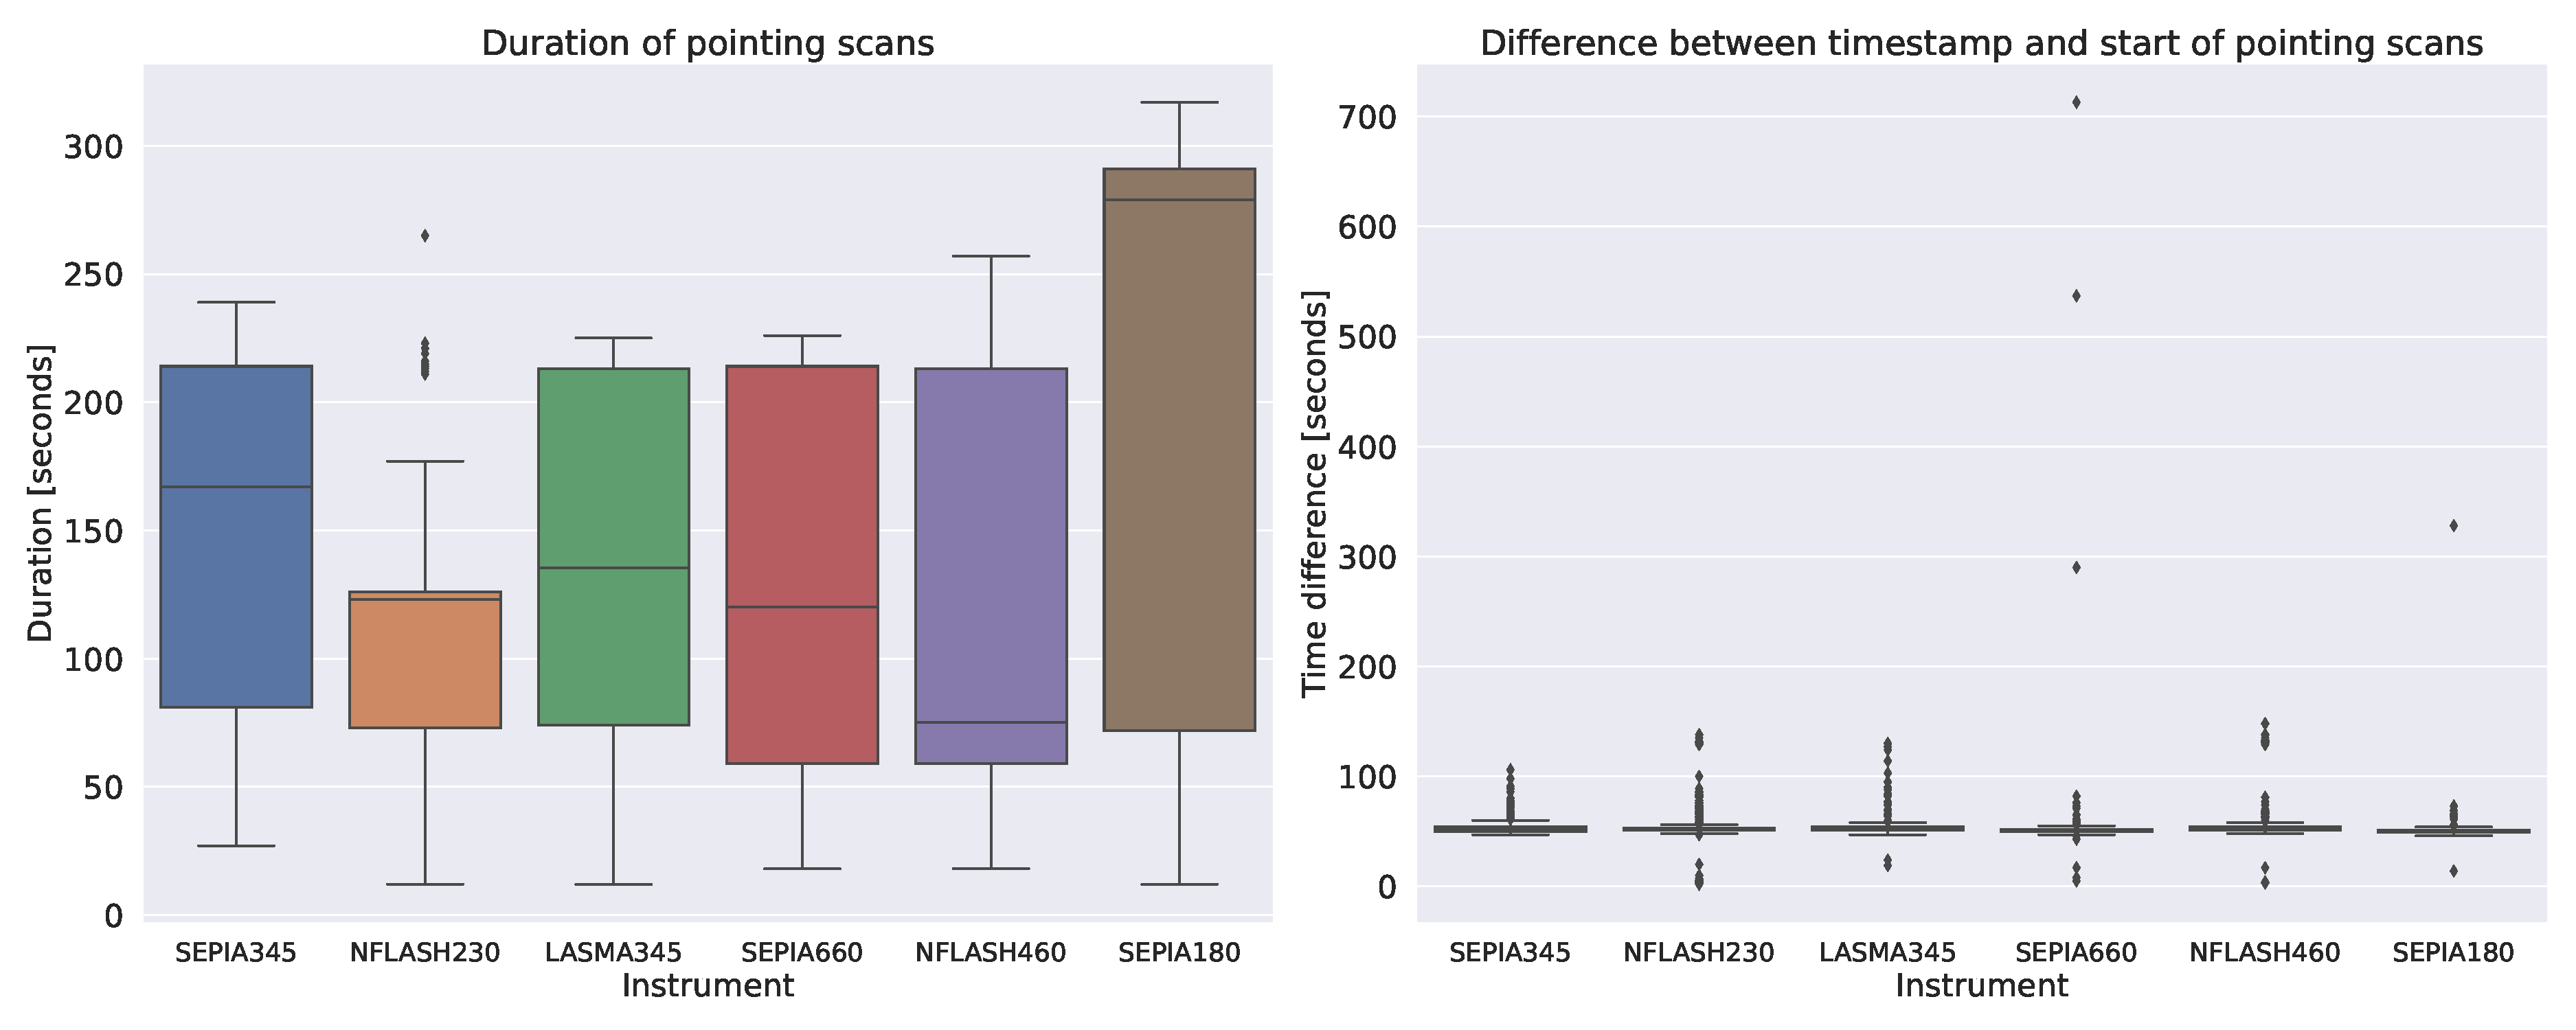
\includegraphics[width=1.1\textwidth]{Tiltmeter plots/scan_duration_distribution_rx.pdf}
    \caption[Box plots with pointing scan duration and start time]{Box plot of the duration of scans, and the time difference between the timestamp of a scan and the actual start of it.}
    \label{fig:scan_times_box}
\end{figure}

\begin{figure}[H]
    \centering
    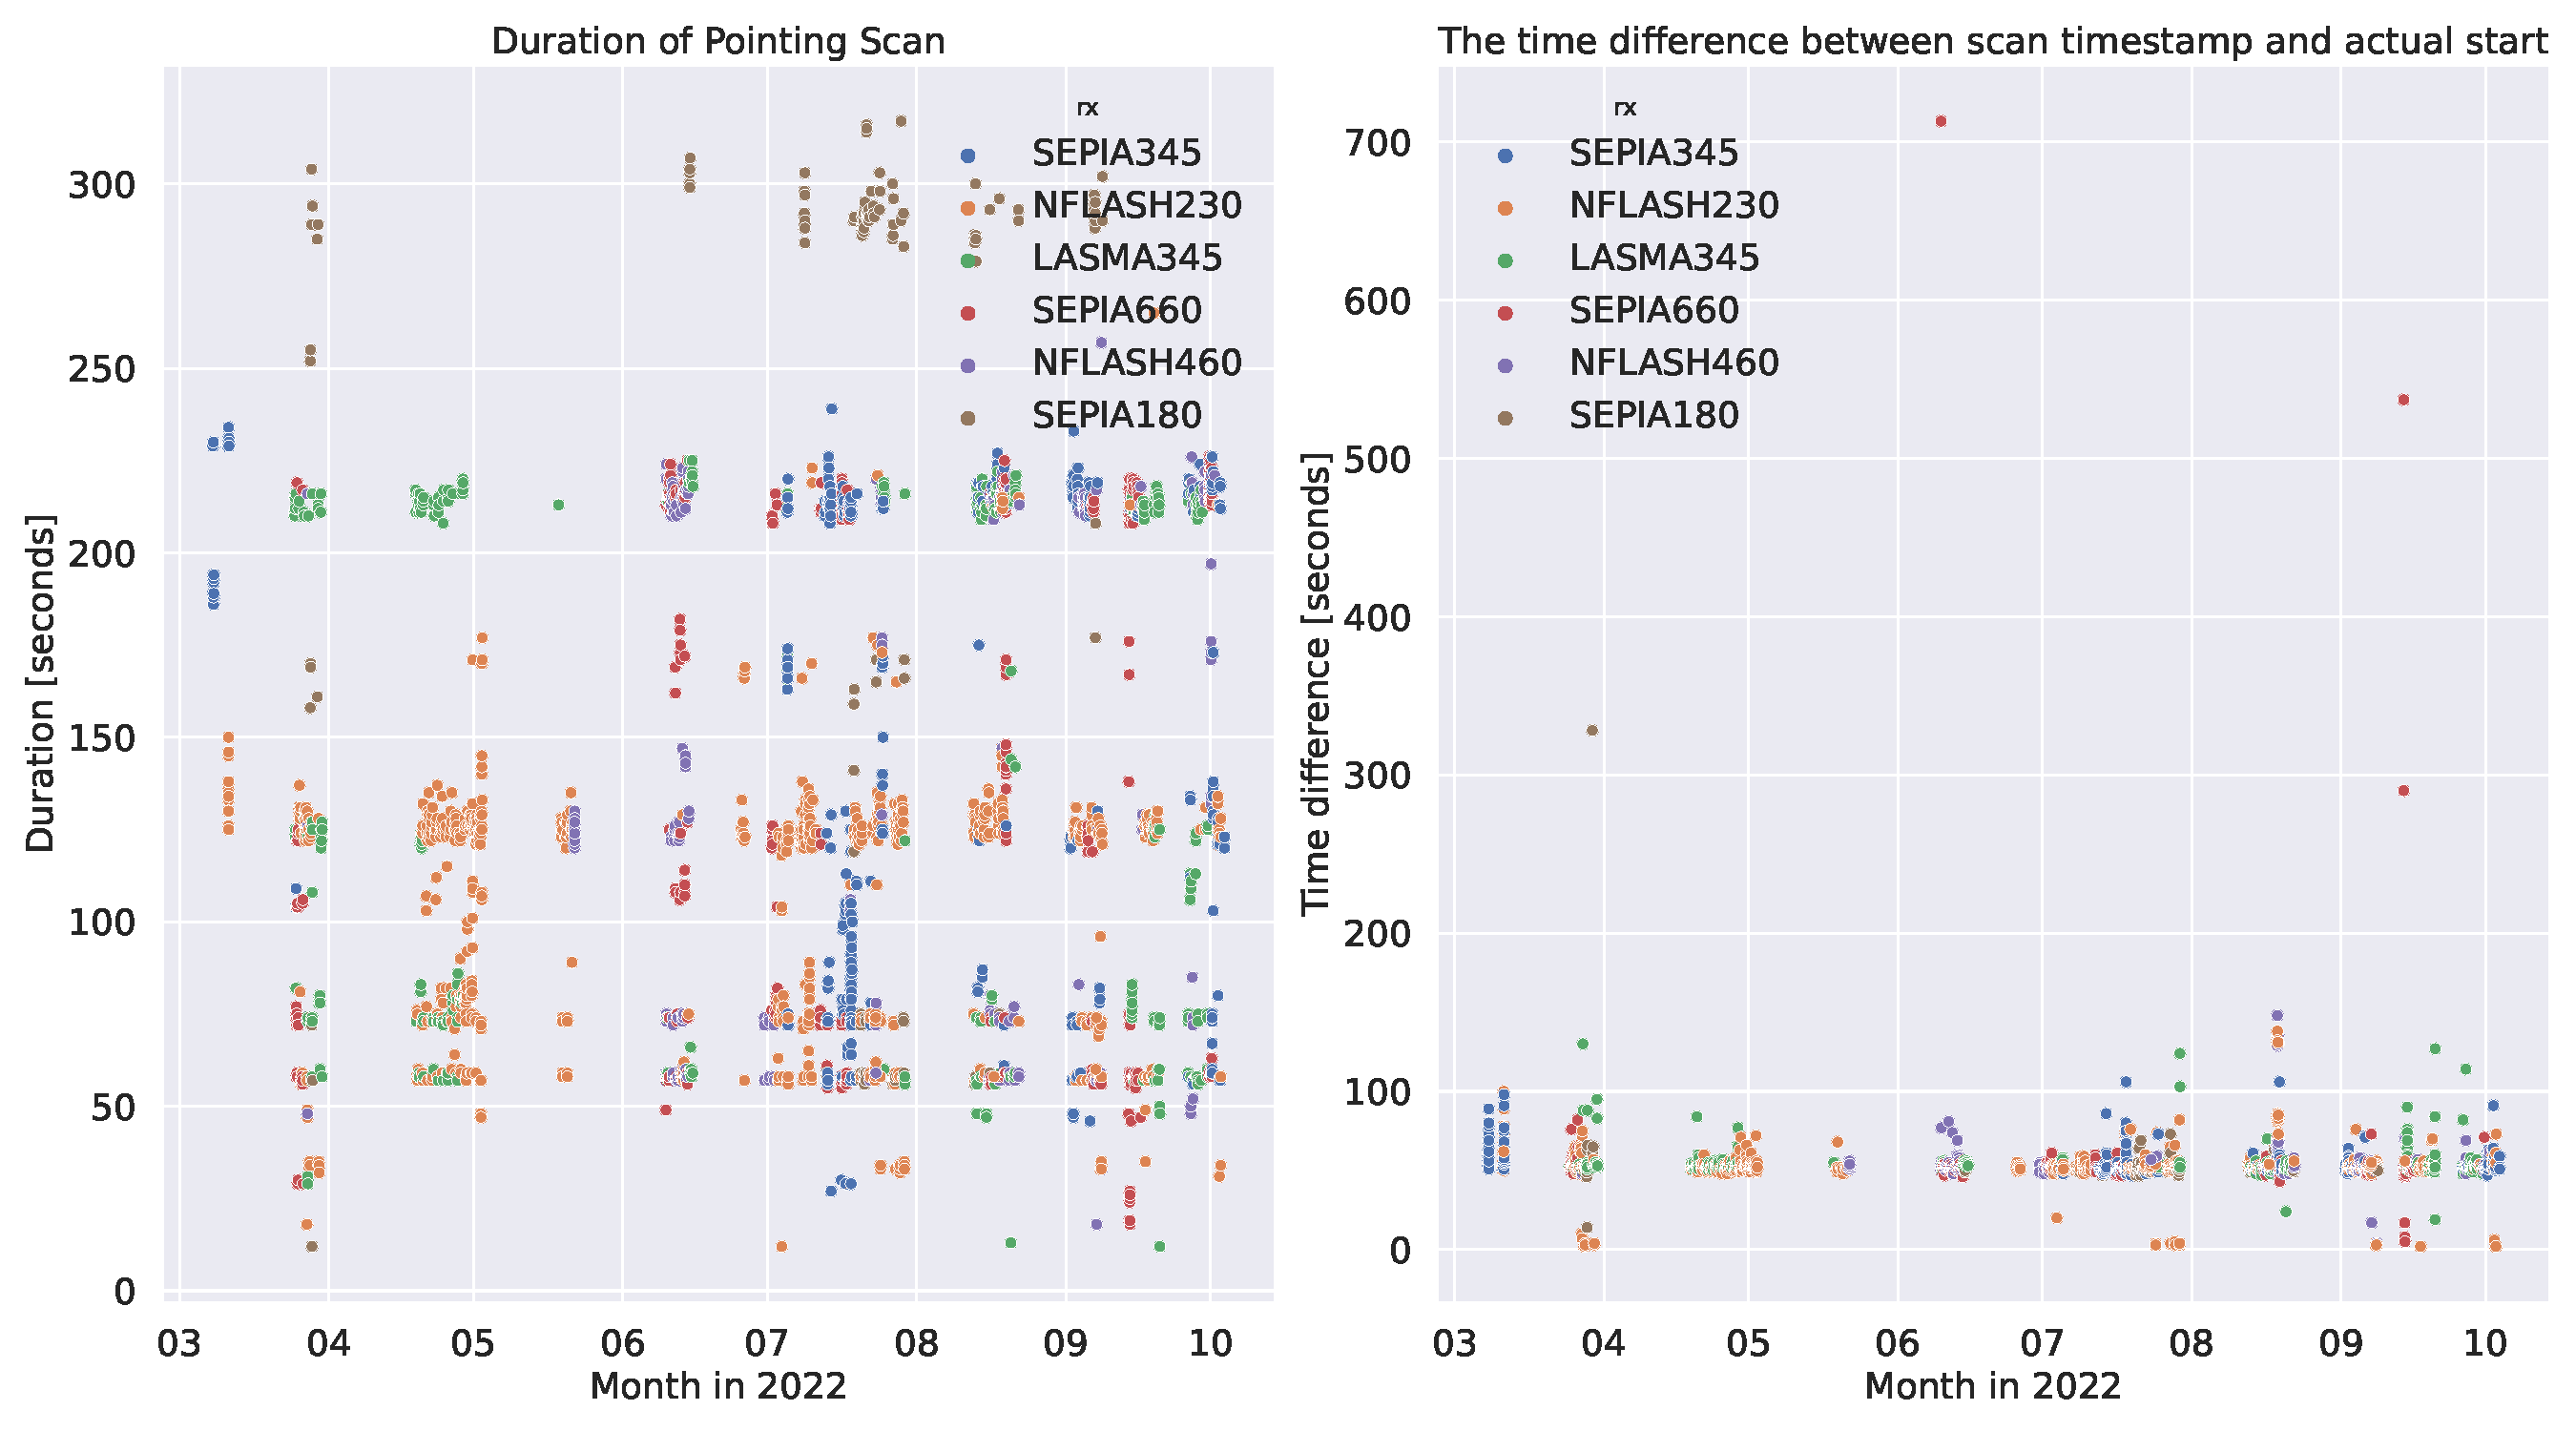
\includegraphics[width=1.1\textwidth]{Tiltmeter plots/scan_duration_distribution_date.pdf}
    \caption[Scatter plot with pointing scan duration and start time throughout 2022.]{Scatter plot of the duration of scans, and the time difference between the timestamp of a scan and the actual start of it.}
    \label{fig:scan_times_date}
\end{figure}


\section{Feature Engineering}\label{sec:feature_engineering}
Feature engineering is important to ensure that the inputs for the machine learning models are as informative as possible.
Informative features make it easier for the machine learning model to learn the relationship between features and target values.
With limited training data, this is essential.

% \textcolor{red}{Put this in feature engineering section}
% \begin{align}
%     \Delta \textit{Az}_\textit{wind} = \textit{Az}_\textit{pointing} - \textit{Az}_\textit{wind}
% \end{align}

% For the turbulence, a simple model is used
% \begin{align}
% v_\textit{wind} = \sigma_\textit{wind}^2
% \end{align}

\subsection{Median Values}
From the scan duration analysis \ref{sec:scan_duration_analysis}, we know that the duration of a scan varies.
Therefore, we use the median value during a pointing scan as a feature.

\subsection{Turbulence}
Turbulence could affect the pointing, and we used the simple model
\begin{align}
\tau_\textit{wind} = \sigma_\textit{wind}^2,
\end{align}
where the $\sigma_\textit{wind}^2$ variance in windspeed.
We calculated the variance in a period of $5$ minutes before the pointing scan.

\subsection{Position of the Sun}
Observers at the telescope report that the sun is affecting the pointing.
It is most drastically affected when the sun sets or rises, likely due to rapid temperature change leading to deformation in the telescope structure.
We also think the sun's position affects the pointing.
For instance, if the sun is shining on the left side of the telescope, it will affect the pointing differently than if it is on the right side.
Obtaining the Sun's position for the telescope's location is done using the Python module PyEphem \cite{ephem}.

Using the azimuth angle of the sun and the telescope, we can calculate the position of the sun with respect to the pointing with
\begin{equation}\label{eq:sun_az_diff}
    \Delta \textit{Az}_\odot = \textit{Az}_{\textit{t}} - \textit{Az}_\odot
\end{equation}
This will result in values outside the $[-180^\circ,180^\circ]$. An example is if $Az_\odot=179^\circ$ and $Az_t = -179^\circ$.
The calculation in equation \eqref{eq:sun_az_diff} yield $-179^\circ-179^\circ=-358^\circ$,
which corresponds to the sun being $358^\circ$ to the right of the telescope, while it ideally should be $2^\circ$ to the left.
Therefore, we adjust the values accordingly
%Write equations where \Delta Az_\odot above 180 is -= 360 and under 180 is += 360
\begin{align}
    \Delta Az_\odot = Az_\odot +360^\circ, \; \text{for} \; \Delta Az_\odot < 180^\circ\\
    \Delta Az_\odot = Az_\odot -360^\circ, \; \text{for} \; \Delta Az_\odot > 180^\circ
\end{align}

Here, the interval of the difference in azimuth is fixed to the interval $(-180^\circ,180^\circ)$,
where $0^\circ$ means the telescope is pointing towards the sun in the azimuth direction.
$\Delta \textit{Az}_\odot = 90^\circ$ corresponds to the sun being direct to the left of the pointing direction.

We also calculated the change of $\Delta Az_\odot$ in the past five minutes.
Let $\Delta Az_\odot(t)$ denote the difference between the telescope's and the Sun's azimuth given time $t$ in minutes,
then the change in the past five minutes are given by
\begin{equation}
    \Delta_5 \Delta Az_\odot=\Delta Az_\odot(t)-\Delta Az_\odot(t-5)
\end{equation}

\subsection{Time based features}
We also used time-based features to capture the time of day and year.
There are seasonal changes that affect the pointing throughout the year, and there are environmental factors throughout the day that are correlated with the time of day.
Therefore, we also used these features
\begin{itemize}
    \item \textbf{Continous month}: The number of months after 2022-01-01 00:00:00
    \item \textbf{Integer month}: The number of integer months after 2022-01-01 00:00:00 
    \item \textbf{Time of day}: The number of hours after 00:00:00 the given day
\end{itemize}

\subsection{Additional features}
There are additional features from the pointing scan data that we used as features.
The correction terms $CA$ \eqref{eq:ca} for azimuth and $IE$ \eqref{eq:ie} for elevation are used as inputs when predicting pointing offsets.
In addition, we used the type of receiver as input.
The environmental factors that cause pointing offsets might affect the different receivers differently; therefore, the model must consider this possibility.


% \begin{table}[H]
%     \centering
%     \caption{Example from the dataset of the observed pointing offsets and the corrections applied during the pointing scan.}
%     \label{tab:offset_and_correction}
%     \begin{tabular}{ccccc}
%     \toprule
%     $i$ &  $\delta_{az}$ &  $\delta_{el}$ &  $ca$ & $ie$  \\
%     \midrule
%     1 & 1.2 & 0.1 & 2.1 &  1.7 \\
%     2 &     0.0 & 0.5 & 3.3 &  1.6 \\
%     3 &    -1.1 & 0.0 & 3.3 &  1.6 \\
%     4 &     0.6 & 0.7 & 2.2 &  1.6 \\
%     5 &     0.9 & 1.4 & 2.2 &  1.6 \\
%     6 &     1.0 & 1.1 & 2.2 &  1.6 \\
%     7 &    -0.9 & 1.2 & 3.1 &  0.5 \\
%     8 &     0.5 & 1.5 & 2.2 & -0.7 \\
%     9 &    -0.3 & 0.4 & 2.2 & -0.7 \\
%     \bottomrule
%     \end{tabular}
% \end{table}


% \begin{table}[H]
%     \centering
%     \caption{Table of transformed pointing offsets and corrections according to equations \eqref{eq:ca_tilde}, \eqref{eq:ie_tilde}, \eqref{eq:off_az_tilde}, and \eqref{eq:off_el_tilde}.}
%     \label{tab:tranform_offsets}
% \begin{tabular}{ccccc}
% \toprule
% $i$ & $\Tilde{\delta}_{az}$ &  $\Tilde{\delta}_{el}$ &  $\Tilde{ca}$ &  $\Tilde{ie}$ \\
% \midrule
% 0 &       1.2 &       0.1 &       2.1 &       1.7 \\
% 1 &       0.0 &       0.5 &       3.3 &       1.6 \\
% 2 &      -1.1 &      -0.5 &       3.3 &       1.1 \\
% 3 &       0.7 &       0.7 &       2.2 &       1.6 \\
% 4 &       0.2 &       0.7 &       2.8 &       0.9 \\
% 5 &       0.1 &      -0.3 &       3.1 &       0.2 \\
% 6 &      -1.0 &       1.3 &       3.2 &       0.5 \\
% 7 &       0.5 &       1.4 &       2.2 &      -0.7 \\
% 8 &      -0.8 &      -1.1 &       2.7 &      -2.2 \\
% \bottomrule
% \end{tabular}
% \end{table}

\label{sec:data_processing}

\chapter{Machine Learning Experiments}

This chapter provides an overview of two machine learning experiments related to the two research questions in section \ref{sec:introduction}.
The first experiment aims to examine the effectiveness of an XGBoost model in predicting pointing scan offsets to enhance the pointing accuracy.
The primary objective of this experiment is to assess whether the proposed model can outperform the current model in terms of pointing accuracy.
The second experiment aims to investigate the effectiveness of neural networks in developing a pointing model that could replace the current linear model, which is created through linear regression.
It explores the feasibility of a more sophisticated model that can account for environmental factors in addition to the theoretical and empirical terms used in the current pointing model.

\section{Experiment 1: Pointing Correction Model} \label{sec:exp1}
This experiment aims to improve the accuracy of the existing pointing model by training XGBoost models to predict offsets obtained from pointing scans.
To accomplish this, we utilized two different datasets, which we processed using the cleaning outlined in section \ref{sec:cleaning_pt_scan}.
The difference between these datasets is that one contains the scans from all instruments, while the other only contains the scans from NFLASH230.
By training our models on these datasets, we aim to reduce the pointing offset and improve the accuracy of the pointing.
In addition, we varied the way we split the datasets for training and testing.
We considered two cases:

\begin{itemize}
    \item \textbf{Case 1:} The dataset is sorted by date and split into six equal-sized folds.
    We consider each of the folds one by one.
    For each of these folds, we use the last $1/6$th of the data as a test set and the remaining $5/6$th as training and validation.
    \item \textbf{Case 2:} The dataset is sorted by date and split into six equal-sized folds.
    We used $5/6$ of the data for training and validation and the remaining for testing.
    We repeated this process six times, using each fold for testing once.
\end{itemize}

Figure \ref{fig:datasplit_cases} illustrates the two cases.
In both cases, we trained and validated the model on $5/6$ of the data and tested on the last $1/6$.
The difference is the amount of data used for training, which can indicate whether models trained on shorter or longer periods perform better.
Using longer period, and thus more data, can help the model find complex relations.
However, a smaller period may be better for learning some relationships, as we expect less variation in a shorter period.

We also split the training and validation data such that scans from a given day only can be either in the training or validation set, not both.
When splitting the data, we used $35\%$ of the days for validation and $65\%$ for training.


\begin{figure}[H]
    \centering
    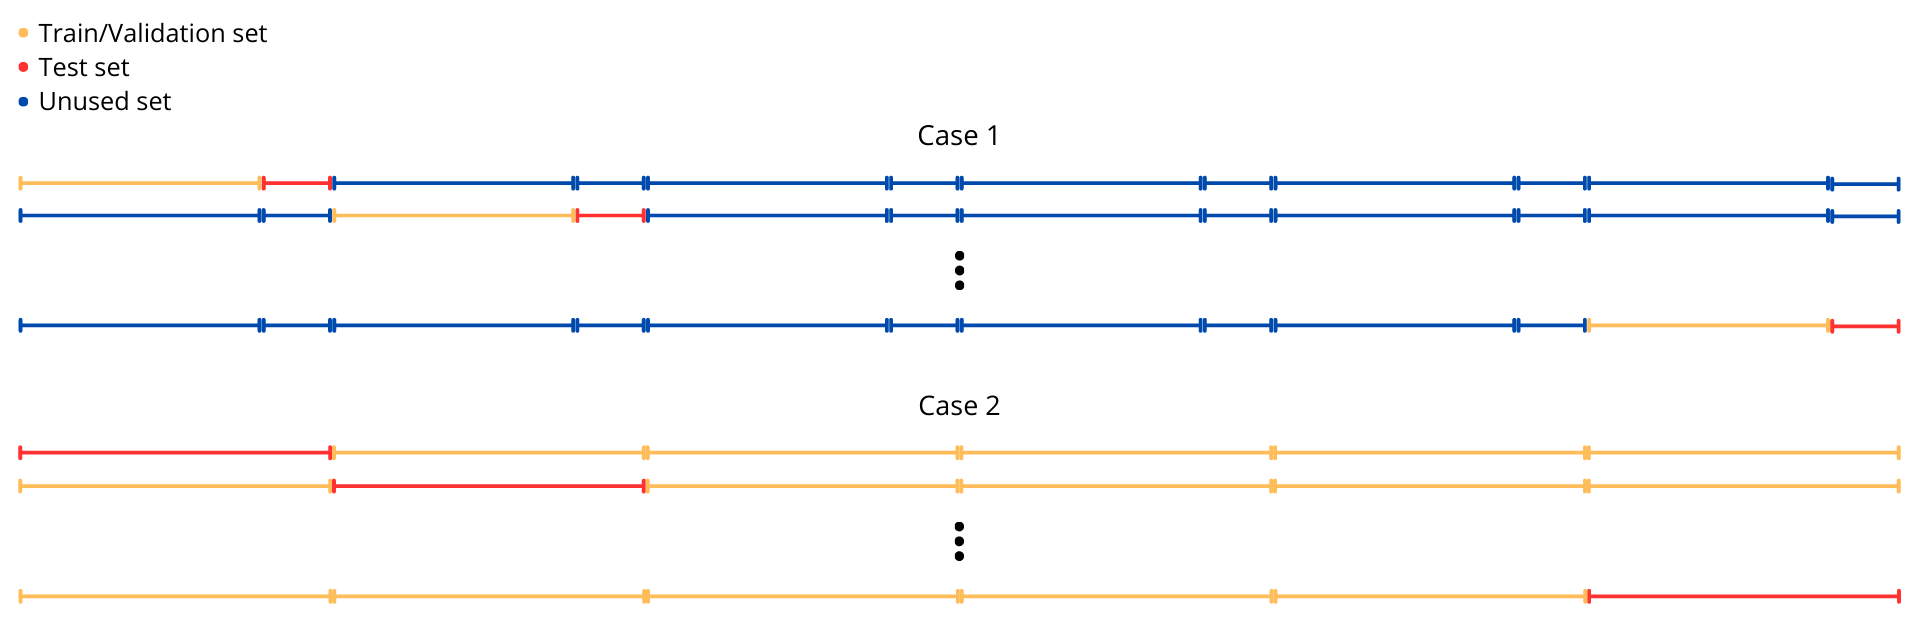
\includegraphics[width=0.98\textwidth]{Canva/datasplits.png}
    \caption[Data split cases for pointing correction model]{This figure shows two cross-validation cases: the orange region represents the train and validation set, the red region represents the test set, and the blue region is unused for evaluation.
    In \textbf{Case 1}, the dataset is split into six equal-sized folds sorted by date.
    For the selected fold, we use the last part (colored red) for testing and the remaining part (colored orange) for training and validation.
    This process is repeated six times, once for each fold.
    In \textbf{Case 2}, the dataset is again split into six equal-sized folds sorted by date.
    However, we use one whole fold for testing this time and the remaining five for training and validation.
    This process is repeated six times, with each fold used exactly once for testing.}
    \label{fig:datasplit_cases}
\end{figure}




\subsection{Feature Selection}
We trained models using a range of features, specifically $k=[2,5,10,20,30,40,50]$ features.
For each model, we selected the $k$ features that had the greatest mutual information \eqref{eq:mutual_info} with the target value on the training and validation set.
This approach helps us identify the most important features to improve the model's performance. Selecting a subset of features can reduce the noise in the data. 
By selecting different numbers of features, we can explore the trade-off between model complexity and performance.

\subsection{Model Architecture}
We performed a hyperparameter search for each model using the parameter space in Table \ref{tab:xgb_hyperparameters_pcorr}.
The search space includes eight hyperparameters that affect the model's complexity, such as the maximum depth of the trees, the regularization strength, and the learning rate.
We used a uniform or log-uniform distribution to sample each hyperparameter within a specific range.
We evaluated $200$ different combinations of hyperparameters (for each dataset, cross-validation case, target variable, and the number of features selected) to find the optimal values for each model.
The models were validated using the MSE.

\begin{table}[H]
    \centering
    \caption[Hyperparameter search space for XGBoost pointing correction model]{This table presents a list of parameters we sampled during hyperparameter tuning for XGBoost the pointing correction model. The table includes names, sampled distributions, and corresponding ranges.}
    \begin{tabular}{lcc}
        \toprule
        \textbf{Parameter} & \textbf{Sample Distribution} & \textbf{Range} \\ \hline
        \texttt{max\_depth} & Uniform & [$1$, $5$] \\ 
        \texttt{reg\_lambda} & Uniform & [$0$, $1$] \\ 
        \texttt{colsample\_bytree} & Uniform & [$0.5$, $1$] \\ 
        \texttt{n\_estimators} & Uniform & [$20$, $500$] \\ 
        \texttt{learning\_rate} & Log-Uniform & [$10^{-5}$, $1$] \\ 
        \texttt{subsample} & Uniform & [$0.5$, $1$] \\ 
        \texttt{gamma} & Log-Uniform & [$10^{-5}$, $1$] \\ 
        \texttt{min\_child\_weight} & Uniform & [$1$, $10$] \\ 
        \bottomrule
    \end{tabular}
    \label{tab:xgb_hyperparameters_pcorr}
\end{table}



\subsection{Model Evaluation}
To evaluate the performance of the models, we calculated the RMS on each test fold and compared it to the current RMS of the telescope on the same data.
We calculated the RMS for azimuth and elevation separately since an XGBoost model only can predict one target.
Given fold $j$ and target either azimuth or elevation, we calculate the RMS by
\begin{equation}
    RMS_{\text{target},j} = \sqrt{\frac{1}{N_j}\sum_{i=1}^{N_j} (\tilde{\delta}_{\text{target},ji} - \delta_{\text{target},ji})^2},
\end{equation}
where $\tilde{\delta}_{\text{target},ji}$ is the predicted pointing offset and $\delta_{\text{target},ji}$ is the true pointing offset for the $i$th pointing scan in fold $j$.
$N_j$ is the number of pointing scans in fold $j$. 

The measure we used for evaluating an analyzing the results is the RMS ratio between the XGBoost pointing correction model and the current model, given by
\begin{equation}\label{eq:rms_compared}
    r_{RMS,j} = \frac{RMS_{\text{target},j}}{RMS_{\text{current},j}}.
\end{equation}
This measure is useful because it compares our results to the current performance of the telescope.
If $r_{RMS,j}<1$, it indicates that the XGBoost model provides an improvement over the current performance of the telescope for a given fold.

To obtain an overall measure of the model's performance compared to the current performance of the telescope, we averaged the ratios $r_{RMS,j}$ over all six test folds
\begin{equation} \label{eq:mean_rms_compared}
    \bar{r}_{RMS} = \sum_{i=1}^6 \frac{RMS_{model,j}}{RMS_{current,j}}.
\end{equation}
This gives us an average ratio $\bar{r}_{RMS}$, which measures the expected performance of the pointing correction model.
If $\bar{r}_{RMS} < 1$, it indicates that the XGBoost model outperforms the current pointing correction method on average across all test folds.
By comparing the average ratio $\bar{r}_{RMS}$ for the two different cross-validation cases in Figure \ref{fig:datasplit_cases},
we can identify which models provide the best performance.



\section{Experiment 2: Pointing Model using Neural Networks}
This experiment uses the raw dataset containing input coordinates, $Az_{\text{input}}$ and $El_{\text{input}}$ respectively, and corresponding true observed values $Az_{\text{observed}}$ and $El_{\text{observed}}$.

The goal is to find a model $f$ such that
\begin{equation}\label{eq:pmodel_f}
    f(X) \approx (\delta_{\text{Az}}, \delta_{\text{El}}) = (Az_{\text{observed}}-Az_{\text{input}}, El_{\text{observed}}-El_{\text{input}})
\end{equation}

We split the data into a train, validation, and test set.
The last $15\%$ of the data, which we sorted by date, is used for testing.
We use the remaining $85\%$ of the data for training and validation and split this set into $20\%$ for training and $80\%$ for validation.
This results in $\sim 76\%$ and $\sim 24\%$ of the total dataset used for training and validation.

\subsection{Feature Selection}
Selecting the right features is essential in improving the pointing model's accuracy.
This model uses two types of features: geometric and harmonic terms (some of which are part of the current analytical pointing model [\eqref{eq:analytical_az},\eqref{eq:analytical_el}]) and new features extracted from the telescope's database.
For the geometric and harmonic terms, we analyzed Pearson and Spearman's rank correlation to the target values in equation \eqref{eq:pmodel_f} and picked a subset of features that showed a strong correlation. 
We did the same for the other features, except we picked out the features that showed a correlation of either type larger than $0.1$.
Tables \ref{tab:raw_data_spearmans} and \ref{tab:raw_data_pearson} list the features we extracted from the database with a correlation equal to or greater than $0.1$.
During model training, we randomly selected $n \in [2, 19] \cap \mathbb{Z}$ features from these lists and used them to train the model.
This way of choosing features does not consider complex dependencies between the features that can affect the offsets.
However, training neural networks is computationally heavy, so we had to select the features we tested carefully.

\subsection{Model Architecture}
This experiment utilized four different model architectures.
The first architecture involved feeding all input data into one or two hidden layers.
The other three architectures incorporated machine learning techniques by separating the geometric and harmonic terms of the input data from the other features and processing them using distinct architectures.
The approaches aimed to keep the current model's simplicity and performance while incorporating new features.

The following are the four different architectures:
\begin{enumerate}
    \item \textbf{Regular Neural Network:} All features are passed through the same layers, all with a nonlinear activation function.
    See Figure \ref{subfig:regular}
    \item \textbf{Neural Network with Separated Features 1:} This architecture separates the input features into two groups: geometric and harmonic features and the rest of the features.
    The geometric and harmonic features are connected directly to the linear output layer, while we pass the remaining features through layers with nonlinear activation functions.
    See Figure \ref{subfig:comb_sep1}
    \item \textbf{Neural Network with Separated Features 2:} This architecture is similar to the previous architecture,
    but we feed the geometric and harmonic features through an additional layer with a nonlinear activation function before connecting them to the output layer.
    See Figure \ref{subfig:comb_sep2}
    \item \textbf{Neural Network with Separated Features 3:} This architecture combines the previous two architectures by passing the regular features through a few hidden layers with nonlinear activation functions before concatenating them with the geometric and harmonic features.
    We then pass the combined features through a final layer before connecting them to the output layer.
    See Figure \ref{subfig:comb_sep3}
\end{enumerate}
These are visualized in Figure \ref{fig:nn_architecture}.

\begin{figure}[H]
    \centering
    \begin{subfigure}[t]{0.49\textwidth}
        \centering
        % NEURAL NETWORK no text - large
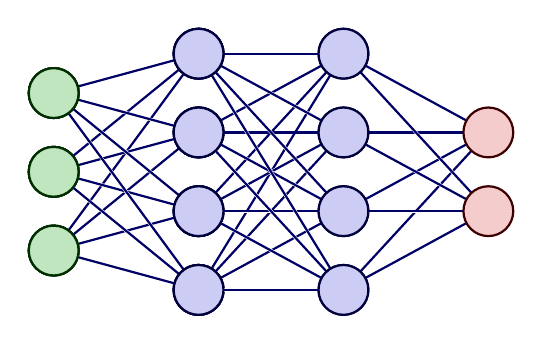
\begin{tikzpicture}[x=2.3cm,y=1.0cm]
  \message{^^JNeural network large}
  \readlist\Nnod{3,4,4,2} % array of number of nodes per layer
  
  \message{^^J  Layer}
  \foreachitem \N \in \Nnod{ % loop over layers
    \def\lay{\Ncnt} % alias of index of current layer
    \pgfmathsetmacro\prev{int(\Ncnt-1)} % number of previous layer
    \message{\lay,}
    \foreach \i [evaluate={\y=\N/2-\i; \x=\lay*0.8; \n=\nstyle;
                           \nprev=int(\prev<\Nnodlen?min(2,\prev):3);}] in {1,...,\N}{ % loop over nodes
      
      % NODES
      %\node[node \n,outer sep=0.6,minimum size=18] (N\lay-\i) at (\x,\y) {};
      \coordinate (N\lay-\i) at (\x,\y);
      
      % CONNECTIONS
      \ifnum\lay>1 % connect to previous layer
        \foreach \j in {1,...,\Nnod[\prev]}{ % loop over nodes in previous layer
          \draw[connect,white,line width=1.2] (N\prev-\j) -- (N\lay-\i);
          \draw[connect] (N\prev-\j) -- (N\lay-\i);
          %\draw[connect] (N\prev-\j.0) -- (N\lay-\i.180); % connect to left
          \node[node \nprev,minimum size=18] at (N\prev-\j) {}; % draw node over lines
        }
        \ifnum \lay=\Nnodlen % draw last node over lines
          \node[node \n,minimum size=18] at (N\lay-\i) {};
        \fi
      \fi % else: nothing to connect first layer
      
    }
  }
  
\end{tikzpicture}
        \caption{\textbf{Regular neural network:}
        This is the standard neural network architecture without any feature separation.
        All features are connected to the same layers.}
        \label{subfig:regular}
    \end{subfigure}
    \hfill
   \begin{subfigure}[t]{0.49\textwidth}
       \centering
       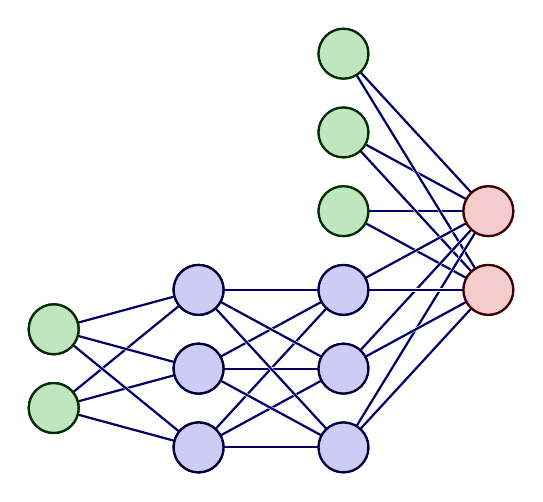
\begin{tikzpicture}[x=2.3cm,y=2.0cm]
  \message{^^JNeural network large}
  \readlist\Nnod{3,2} % array of number of nodes per layer
  \readlist\Nnodtwo{2,3,3,2}
  \message{^^J  Layer}
  \foreachitem \N \in \Nnod{ % loop over layers
    \def\lay{\Ncnt} % alias of index of current layer
    \pgfmathsetmacro\prev{int(\Ncnt-1)} % number of previous layer
    \message{\lay,}
    \foreach \i [evaluate={\y=\N/4-\i*0.5; \x=\lay*0.8+1.6; \n=\nstyle;
                           \nprev=int(\prev<\Nnodlen?min(2,\prev):3);}] in {1,...,\N}{ % loop over nodes
      
      % NODES
      %\node[node \n,outer sep=0.6,minimum size=18] (N\lay-\i) at (\x,\y) {};
      \ifnum \lay<\Nnodlen % draw last node over lines
        \coordinate (N\lay-\i) at (\x,\y);
      \else
        \coordinate (N\lay-\i) at (\x,\y-0.75);
      \fi
      % CONNECTIONS
      \ifnum\lay>1 % connect to previous layer
        \foreach \j in {1,...,\Nnod[\prev]}{ % loop over nodes in previous layer
          \draw[connect,white,line width=1.2] (N\prev-\j) -- (N\lay-\i);
          \draw[connect] (N\prev-\j) -- (N\lay-\i);
          %\draw[connect] (N\prev-\j.0) -- (N\lay-\i.180); % connect to left
          \node[node \nprev,minimum size=18] at (N\prev-\j) {}; % draw node over lines
        }
        \ifnum \lay=\Nnodlen % draw last node over lines
          \node[node \n,minimum size=18] at (N\lay-\i) {};
        \fi
      \fi % else: nothing to connect first layer
      
    }
  }

  \foreachitem \N \in \Nnodtwo{ % loop over layers
    \def\lay{\Ncnt} % alias of index of current layer
    \pgfmathsetmacro\prev{int(\Ncnt-1)} % number of previous layer
    \message{\lay,}
    \foreach \i [evaluate={\y=\N/4-\i*0.5-1.5; \x=\lay*0.8; \n=\nstyle;
                           \nprev=int(\prev<\Nnodtwolen?min(2,\prev):3);}] in {1,...,\N}{ % loop over nodes
      % NODES
      %\node[node \n,outer sep=0.6,minimum size=18] (N\lay-\i) at (\x,\y) {};
      \ifnum \lay<\Nnodtwolen % draw last node over lines
        \coordinate (M\lay-\i) at (\x,\y);
      \else
        \coordinate (M\lay-\i) at (\x,\y+0.75);
      \fi
      % CONNECTIONS
      \ifnum\lay>1 % connect to previous layer
        \foreach \j in {1,...,\Nnodtwo[\prev]}{ % loop over nodes in previous layer
          \draw[connect,white,line width=1.2] (M\prev-\j) -- (M\lay-\i);
          \draw[connect] (M\prev-\j) -- (M\lay-\i);
          %\draw[connect] (N\prev-\j.0) -- (N\lay-\i.180); % connect to left
          \node[node \nprev,minimum size=18] at (M\prev-\j) {}; % draw node over lines
        }
        \ifnum \lay=\Nnodtwolen % draw last node over lines
          \node[node \n,minimum size=18] at (M\lay-\i) {};
        \fi
      \fi % else: nothing to connect first layer
      
    }
  }
  
\end{tikzpicture}
       \caption{\textbf{Neural network with separated features 1:}
       In this architecture, the geometric and harmonic features are separated from the other features and directly connected to the output layer without any nonlinear activation function.}
       \label{subfig:comb_sep1}
\end{subfigure}
\\~\\
    \begin{subfigure}[t]{0.49\textwidth}
        \centering
        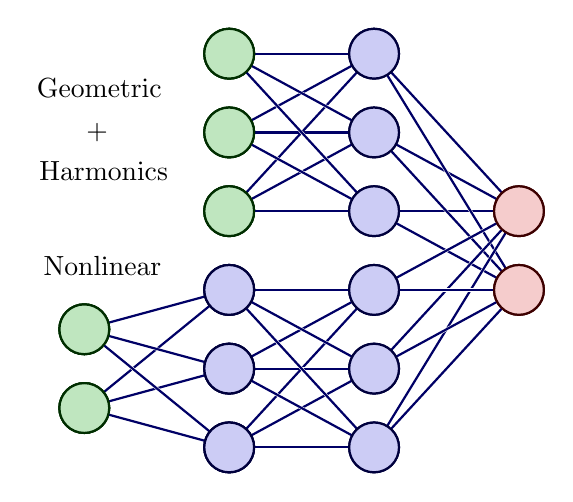
\begin{tikzpicture}[x=2.3cm,y=2.0cm]
  \message{^^JNeural network large}
  \readlist\Nnod{3,3,2} % array of number of nodes per layer
  \readlist\Nnodtwo{2,3,3,2}
  \message{^^J  Layer}
  \foreachitem \N \in \Nnod{ % loop over layers
    \def\lay{\Ncnt} % alias of index of current layer
    \pgfmathsetmacro\prev{int(\Ncnt-1)} % number of previous layer
    \message{\lay,}
    \foreach \i [evaluate={\y=\N/4-\i*0.5; \x=\lay*0.8+0.8; \n=\nstyle;
                           \nprev=int(\prev<\Nnodlen?min(2,\prev):3);}] in {1,...,\N}{ % loop over nodes
      
      % NODES
      %\node[node \n,outer sep=0.6,minimum size=18] (N\lay-\i) at (\x,\y) {};
      \ifnum \lay<\Nnodlen % draw last node over lines
        \coordinate (N\lay-\i) at (\x,\y);
      \else
        \coordinate (N\lay-\i) at (\x,\y-0.75);
      \fi
      % CONNECTIONS
      \ifnum\lay>1 % connect to previous layer
        \foreach \j in {1,...,\Nnod[\prev]}{ % loop over nodes in previous layer
          \draw[connect,white,line width=1.2] (N\prev-\j) -- (N\lay-\i);
          \draw[connect] (N\prev-\j) -- (N\lay-\i);
          %\draw[connect] (N\prev-\j.0) -- (N\lay-\i.180); % connect to left
          \node[node \nprev,minimum size=18] at (N\prev-\j) {}; % draw node over lines
        }
        \ifnum \lay=\Nnodlen % draw last node over lines
          \node[node \n,minimum size=18] at (N\lay-\i) {};
        \fi
      \fi % else: nothing to connect first layer
      
    }
  }
  \node[shift = {(-1.5,0)}] at (N2-2){
    $\begin{aligned}
      \text{Geom}&\text{etric}\\
      +&\\
      \text{Harm}&\text{onics}
    \end{aligned}$
  };
  \node[shift = {(-1.5,-0.85)}] at (N2-2){Nonlinear};
  \foreachitem \N \in \Nnodtwo{ % loop over layers
    \def\lay{\Ncnt} % alias of index of current layer
    \pgfmathsetmacro\prev{int(\Ncnt-1)} % number of previous layer
    \message{\lay,}
    \foreach \i [evaluate={\y=\N/4-\i*0.5-1.5; \x=\lay*0.8; \n=\nstyle;
                           \nprev=int(\prev<\Nnodtwolen?min(2,\prev):3);}] in {1,...,\N}{ % loop over nodes
      % NODES
      %\node[node \n,outer sep=0.6,minimum size=18] (N\lay-\i) at (\x,\y) {};
      \ifnum \lay<\Nnodtwolen % draw last node over lines
        \coordinate (M\lay-\i) at (\x,\y);
      \else
        \coordinate (M\lay-\i) at (\x,\y+0.75);
      \fi
      % CONNECTIONS
      \ifnum\lay>1 % connect to previous layer
        \foreach \j in {1,...,\Nnodtwo[\prev]}{ % loop over nodes in previous layer
          \draw[connect,white,line width=1.2] (M\prev-\j) -- (M\lay-\i);
          \draw[connect] (M\prev-\j) -- (M\lay-\i);
          %\draw[connect] (N\prev-\j.0) -- (N\lay-\i.180); % connect to left
          \node[node \nprev,minimum size=18] at (M\prev-\j) {}; % draw node over lines
        }
        \ifnum \lay=\Nnodtwolen % draw last node over lines
          \node[node \n,minimum size=18] at (M\lay-\i) {};
        \fi
      \fi % else: nothing to connect first layer
      
    }
  }
  
\end{tikzpicture}
        \caption{\textbf{Neural network with separated features 2}:
        Similar to the previous architecture, the geometric and harmonic features are separated from the other features.
        However, they are also processed by a nonlinear activation function before being connected to the output layer.}
        \label{subfig:comb_sep2}
    \end{subfigure}
    \hfill
       \begin{subfigure}[t]{0.49\textwidth}
        \centering
        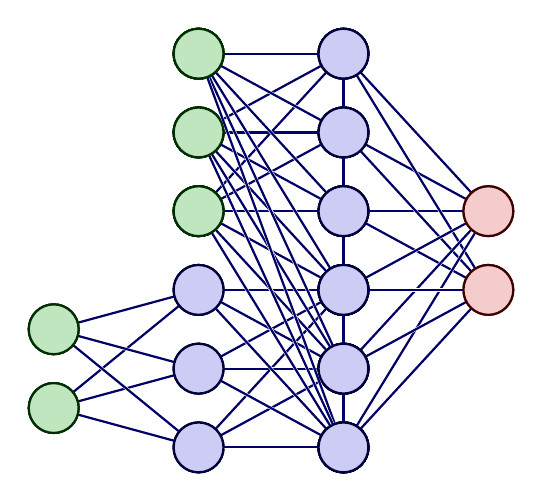
\begin{tikzpicture}[x=2.3cm,y=2.0cm]
  \message{^^JNeural network large}
  \readlist\Nnod{3,3,2} % array of number of nodes per layer
  \readlist\Nnodtwo{2,3,3,2}
  \message{^^J  Layer}
  \foreachitem \N \in \Nnod{ % loop over layers
    \def\lay{\Ncnt} % alias of index of current layer
    \pgfmathsetmacro\prev{int(\Ncnt-1)} % number of previous layer
    \message{\lay,}
    \foreach \i [evaluate={\y=\N/4-\i*0.5; \x=\lay*0.8+0.8; \n=\nstyle;
                           \nprev=int(\prev<\Nnodlen?min(2,\prev):3);}] in {1,...,\N}{ % loop over nodes
      
      % NODES
      %\node[node \n,outer sep=0.6,minimum size=18] (N\lay-\i) at (\x,\y) {};
      \ifnum \lay<\Nnodlen % draw last node over lines
        \coordinate (N\lay-\i) at (\x,\y);
      \else
        \coordinate (N\lay-\i) at (\x,\y-0.75);
      \fi
      % CONNECTIONS
      \ifnum\lay>1 % connect to previous layer
        \foreach \j in {1,...,\Nnod[\prev]}{ % loop over nodes in previous layer
          \draw[connect,white,line width=1.2] (N\prev-\j) -- (N\lay-\i);
          \draw[connect] (N\prev-\j) -- (N\lay-\i);
          %\draw[connect] (N\prev-\j.0) -- (N\lay-\i.180); % connect to left
          \node[node \nprev,minimum size=18] at (N\prev-\j) {}; % draw node over lines
        }
        \ifnum \lay=\Nnodlen % draw last node over lines
          \node[node \n,minimum size=18] at (N\lay-\i) {};
        \fi
      \fi % else: nothing to connect first layer
      
    }
  }

  \foreachitem \N \in \Nnodtwo{ % loop over layers
    \def\lay{\Ncnt} % alias of index of current layer
    \pgfmathsetmacro\prev{int(\Ncnt-1)} % number of previous layer
    \message{\lay,}
    \foreach \i [evaluate={\y=\N/4-\i*0.5-1.5; \x=\lay*0.8; \n=\nstyle;
                           \nprev=int(\prev<\Nnodtwolen?min(2,\prev):3);}] in {1,...,\N}{ % loop over nodes
      % NODES
      %\node[node \n,outer sep=0.6,minimum size=18] (N\lay-\i) at (\x,\y) {};
      \ifnum \lay<\Nnodtwolen % draw last node over lines
        \coordinate (M\lay-\i) at (\x,\y);
      \else
        \coordinate (M\lay-\i) at (\x,\y+0.75);
      \fi
      % CONNECTIONS
      \ifnum\lay>1 % connect to previous layer
        \foreach \j in {1,...,\Nnodtwo[\prev]}{ % loop over nodes in previous layer
          \draw[connect,white,line width=1.2] (M\prev-\j) -- (M\lay-\i);
          \draw[connect] (M\prev-\j) -- (M\lay-\i);
          %\draw[connect] (N\prev-\j.0) -- (N\lay-\i.180); % connect to left
          \node[node \nprev,minimum size=18] at (M\prev-\j) {}; % draw node over lines
        }
        \ifnum \lay=\Nnodtwolen % draw last node over lines
          \node[node \n,minimum size=18] at (M\lay-\i) {};
        \fi
      \fi % else: nothing to connect first layer
      
    }
  }

  \foreachitem \N \in \Nnod{ % loop over layers
    \def\lay{\Ncnt} % alias of index of current layer
    \pgfmathsetmacro\prev{int(\Ncnt-1)} % number of previous layer
    \message{\lay,}
    \foreach \i [evaluate={\y=\N-\i*0.5; \x=\lay; \n=\nstyle;
                           \nprev=int(\prev<\Nnodlen?min(2,\prev):3);}] in {1,...,\N}{ % loop over nodes
      
      % CONNECTIONS
      \ifnum\lay=2 % connect to previous layer
        \foreach \j in {1,...,\Nnod[\prev]}{ % loop over nodes in previous layer
          \draw[connect,white,line width=1.2] (M3-\j) -- (N\lay-\i);
          \draw[connect] (M3-\j) -- (N\lay-\i);
          %\draw[connect] (N\prev-\j.0) -- (N\lay-\i.180); % connect to left
          \message{^^J Nprev \nprev}
          \node[node 2,minimum size=18] at (M3-\j) {}; % draw node over lines
          \node[node 2,minimum size=18] at (N\lay-\j) {}; % draw node over lines
        }
      \fi % else: nothing to connect first layer
      
    }
  }

  \foreachitem \N \in \Nnodtwo{ % loop over layers
    \def\lay{\Ncnt} % alias of index of current layer
    \pgfmathsetmacro\prev{int(\Ncnt-1)} % number of previous layer
    \message{\lay,}
    \foreach \i [evaluate={\y=\N/4-\i*0.5; \x=\lay+2; \n=\nstyle;
                           \nprev=int(\prev<\Nnodtwolen?min(2,\prev):3);}] in {1,...,\N}{ % loop over nodes
      % NODES
      %\node[node \n,outer sep=0.6,minimum size=18] (N\lay-\i) at (\x,\y) {};
      \ifnum\lay=3 % connect to previous layer
        \foreach \j in {1,...,\Nnodtwo[\prev]}{ % loop over nodes in previous layer
          \message{^^J \lay Here (N1-\j) {l\lay}}
          \draw[connect,white,line width=1.2] (N1-\j) -- (M\lay-\i);
          \draw[connect] (N1-\j) -- (M\lay-\i);
          %\draw[connect] (N\prev-\j.0) -- (N\lay-\i.180); % connect to left
          \node[node 1,minimum size=18] at (N1-\j) {}; % draw node over lines
          \node[node 2,minimum size=18] at (M\lay-\j) {}; % draw node over lines
          
        }

      \fi % else: nothing to connect first layer
      
    }
  }



\end{tikzpicture}
        \caption{\textbf{Neural network with separated features 3:}
        In this architecture, we concatenate the processed regular features to the geometric and harmonic features before being connected to the output layer.}
        \label{subfig:comb_sep3}
    \end{subfigure}
     \caption[Neural network architectures for pointing model]{The different architectures tested for the pointing model.}
     \label{fig:nn_architecture}
\end{figure}

The hyperparameters for the neural networks were randomly sampled from different distributions, as presented in Table \ref{tab:nn_hyperparameters}.
We used the Adam optimization algorithm for all models and trained $100$ networks of each architecture for $200$ epochs.
We picked the model from the epoch with the best performance on the validation set.
\begin{table}[H]
    \centering
    \caption[Hyperparameter search space for neural network pointing models]{This table presents a list of parameters we sampled during hyperparameter tuning for the base pointing model. The table includes names, the distribution we sampled from, and corresponding ranges.}
    \begin{tabular}{lcc}
    \hline
    \textbf{Name} & \textbf{Distribution Type} & \textbf{Range} \\ \hline
    hidden layers & uniform integer & [$1$,$3$] \\
    hidden layer size & uniform integer & [$20$, $120$] \\
    learning rate & uniform & [$0.001$, $0.02$] \\
    batch size & uniform integer & [$32$, $512$] \\
    activation & categorical & [gelu, tanh] \\
    loss function & categorical & [MSE \eqref{eq:mse1}, MSD \eqref{eq:msd}] \\ \hline
    \end{tabular}
    \label{tab:nn_hyperparameters}
    \end{table}

\subsection{Loss Function and Model Evaluation}
To evaluate the performance of the models, we used the root mean squared (RMS), measured in arcseconds, on the test set.
We calculate the RMS as follows:
\begin{equation}
    \text{RMS} = \sqrt{ \frac{1}{N} \sum_{i=1}^N \left( (\tilde{\delta}_{Az,i} - \delta_{Az,i})^2 + (\tilde{\delta}_{El,i} - \delta_{El,i})^2 \right)},
\end{equation}
where $\tilde{\delta}_{Az}$ and $\tilde{\delta}_{El}$ are the predicted offsets, while $\delta_{Az}$ and $\delta_{El}$ are the true values.
$N$ is the number of observations in the test set.

This RMS is used to compare the performance of the models.
It will also be compared with a benchmark linear regression model to see if a machine learning approach offers any improvements.


\part{Results \& Discussion}
\chapter{Results \& Discussion}
\section{Results of Experiment 1: Pointing Correction Model}
In this section, we present the results obtained from experiment $1$ introduced in section \ref{sec:exp1}.
Prior to presenting the results, we provide a reminder of the RMS ratio measure \eqref{eq:mean_rms_compared}, which we frequently used in this section.
We used this measure to compare the current pointing model to the machine learning model, and a value less than $1$ indicates an improvement of the current model. \\

Table \ref{tab:results_minval_val_test_days_04_n230} presents the validation and test RMS ratios for all folds of the NFLASH230 model in case 1 and case 2.
Recall that models were trained with different numbers of features $k$, and these results are from the model with the best performance on the validation set (can be different $k$ for each fold).
The results show that the model's performance on the validation set is very good in both case 1 and 2.
However, this does not generalize well to the test set, with the performance on the test set for case 1 being significantly worse than the current model for all folds.
In contrast, for case 2, the performance on the test set is better than the current model for most of the folds.
Table \ref{tab:results_minval_val_test_days_04_all} presents the same results for the model predicting the offsets of all instruments.
This model exhibits similar trends, although its performance on the test set is not as good as the NFLASH230 model.\\

\begin{table}[!htbp]
    \centering
    \caption[NFLASH230 pointing correction model results on each fold]{
    Validation and test performance measured in RMS ratio \eqref{eq:rms_compared} in case 1 and 2 (see Figure \ref{fig:datasplit_cases}) for the pointing correction model trained on NFLASH230 data.
    The performance is given for the model complexity $k$ that yields the best results on the validation data for the given fold.}
    \begin{tabular}{lccccc}
        \toprule
        & & \multicolumn{2}{c}{Case 1 RMS ratio} & \multicolumn{2}{c}{Case 2 RMS ratio} \\
        \cmidrule{3-4} \cmidrule{5-6}
        Target & Fold & Validation & Test &  Validation &  Test \\
        \midrule
        \multirow{6}{*}{Azimuth} & 1 &  0.848 &       1.188 &      0.846 &       1.043 \\
                            & 2 &  0.841 &       1.427 &      0.870 &       0.962 \\
                            & 3 &  0.840 &       1.462 &      0.923 &       0.882 \\
                            & 4 &  0.837 &       1.266 &      0.873 &       0.989 \\
                            & 5 &  0.846 &       1.242 &      0.879 &       0.944 \\
                            & 6 &  0.837 &       1.318 &      0.907 &       0.930 \\
        \hline
        \multirow{6}{*}{Elevation} & 1 &  0.835 &       1.173 &      0.887 &       1.030 \\
                            & 2 &  0.831 &       1.188 &      0.889 &       0.973 \\
                            & 3 &  0.831 &       1.204 &      0.886 &       1.025 \\
                            & 4 &  0.812 &       1.198 &      0.826 &       0.844 \\
                            & 5 &  0.815 &       1.166 &      0.802 &       0.870 \\
                            & 6 &  0.810 &       1.262 &      0.825 &       0.906 \\
        \bottomrule
    \end{tabular}
    \label{tab:results_minval_val_test_days_04_n230}
\end{table}

\newpage 
\begin{table}[!htbp]
    \centering
    \caption[All instruments pointing correction model results on each fold]{
    Validation and test performance measured in RMS ratio \eqref{eq:rms_compared} in case 1 and 2 (see Figure \ref{fig:datasplit_cases}) for the pointing correction model trained on all data.
    The performance is given for the model complexity $k$ that yields the best results on the validation data for the given fold.}
    \begin{tabular}{lccccc}
        \toprule
        & & \multicolumn{2}{c}{Case 1 RMS ratio} & \multicolumn{2}{c}{Case 2 RMS ratio} \\
        \cmidrule{3-4} \cmidrule{5-6}
        Target & Fold & Validation & Test &  Validation &  Test \\
        \midrule
        \multirow{6}{*}{Azimuth} & 1 &  0.870 &       1.642 &      0.881 &       1.233 \\
                            & 2 &  0.861 &       1.626 &      0.971 &       0.928 \\
                            & 3 &  0.876 &       1.784 &      0.897 &       1.016 \\
                            & 4 &  0.866 &       1.613 &      0.938 &       0.950 \\
                            & 5 &  0.862 &       1.935 &      0.927 &       0.942 \\
                            & 6 &  0.874 &       1.779 &      0.923 &       1.027 \\
                            \hline
        \multirow{6}{*}{Elevation} & 1 &  0.832 &       1.193 &      0.948 &       0.965 \\
                            & 2 &  0.831 &       1.141 &      0.924 &       1.051 \\
                            & 3 &  0.824 &       1.129 &      0.929 &       1.094 \\
                            & 4 &  0.816 &       1.172 &      0.822 &       0.922 \\
                            & 5 &  0.818 &       1.196 &      0.828 &       0.978 \\
                            & 6 &  0.822 &       1.186 &      0.831 &       0.951 \\
                            \bottomrule
    \end{tabular}
    \label{tab:results_minval_val_test_days_04_all}
\end{table}


In addition to Table \ref{tab:results_minval_val_test_days_04_n230} and Table \ref{tab:results_minval_val_test_days_04_all},
we also evaluated the performance of the NFLASH230 model with different complexities.
Table \ref{tab:results_nflash_days} shows the mean RMS ratio \eqref{eq:mean_rms_compared} on the test set,
and the associated standard deviation for the azimuth and elevation models when using the same number of features $k$ on all folds.
By inspection, we see that the machine learning model does not provide any improvement over the current pointing model for case 1, apart from a slight improvement of an average of $1.8\%$ reduced RMS with a standard deviation of $1.4\%$ for the azimuth model with number of features $k=2$.
However, case 2 shows more promising results.
For azimuth, the best RMS ratio is $0.948$ with a standard deviation of $0.056$, which is an average improvement of $5.2\%$ reduced RMS on all folds, with a standard deviation of $5.6\%$.
The number of features for these results is $k=2$.
Using $k=50$ features shows similar results, with $0.945$ RMS ratio and a standard deviation of $0.073$.\\

For elevation, the best RMS ratio is $0.940$ with a standard deviation of $0.075$, using $k=50$ features.
Table \ref{tab:results_all_days} shows the same results for case 1 and 2, but for the model trained on data from all instruments.
We see the same trends, with case 1 showing no improvement and case 2 showing a slight improvement for azimuth and elevation.
The best RMS ratio for azimuth in case 2 is $0.980$ with a standard deviation of $0.059$, using $k=2$ features.
For elevation, the best model is the one with $k=50$ features, with a RMS ratio of $0.955$ and a standard deviation of $0.029$.
Overall, the elevation models show slightly better results than the azimuth models.
Additionally, the model predicting only NFLASH230 offsets performs better than the model predicting offsets from all instruments. \\


\begin{table}[!htbp]
    \centering
    \caption[NFLASH230 model results for complexity $k$]{%$tmp2022\_clean\_clf\_nflash230\_results\_table$
    Resulting mean RMS ratio \eqref{eq:mean_rms_compared} on unseen test sets in case $1$ and $2$ (see Figure \ref{fig:datasplit_cases}) for the model trained on NFLASH230 data,
    using different number of features $k$ in the model.}
    \begin{tabular}{ccccc c cccc}
        \toprule
        \multicolumn{1}{c}{} & \multicolumn{4}{c}{Case 1} & & \multicolumn{4}{c}{Case 2} \\
        \cmidrule(lr){2-5} \cmidrule(lr){7-10}
        \multicolumn{1}{c}{} & \multicolumn{2}{c}{Azimuth} & \multicolumn{2}{c}{Elevation} & & \multicolumn{2}{c}{Azimuth} & \multicolumn{2}{c}{Elevation} \\ 
        \cmidrule(lr){2-5} \cmidrule(lr){7-10}
        k & Mean & STD & Mean & STD & & Mean & STD & Mean & STD \\ 
        \midrule
         2 &     0.982 &     0.014 &     1.020 &     0.024 &  &  0.948 &     0.056 &     0.972 &     0.081 \\
         5 &     1.366 &     0.077 &     1.198 &     0.034 &  &  0.983 &     0.142 &     0.953 &     0.097 \\
        10 &     1.383 &     0.087 &     1.155 &     0.047 &  &  0.957 &     0.080 &     0.967 &     0.087 \\
        20 &     1.252 &     0.119 &     1.126 &     0.071 &  &  0.972 &     0.131 &     0.949 &     0.069 \\
        30 &     1.335 &     0.226 &     1.094 &     0.041 &  &  0.963 &     0.093 &     0.959 &     0.077 \\
        40 &     1.146 &     0.036 &     1.058 &     0.020 &  &  0.961 &     0.089 &     0.948 &     0.077 \\
        50 &     1.202 &     0.131 &     1.062 &     0.022 &  &  0.945 &     0.073 &     0.940 &     0.075 \\
        \bottomrule
    \end{tabular}
    \label{tab:results_nflash_days}
\end{table}

\begin{table}[!htbp]
    \centering
    \caption[All instruments model results for complexity $k$]{%$tmp2022\_clean\_clf\_results\_table$
    Resulting mean RMS ratio \eqref{eq:mean_rms_compared} on unseen test sets in case $1$ and $2$ (see Figure \ref{fig:datasplit_cases}) for the model trained on all data,
    using different number of features $k$ in the model.}
    \begin{tabular}{ccccc c cccc}
        \toprule
        \multicolumn{1}{c}{} & \multicolumn{4}{c}{Case 1} & & \multicolumn{4}{c}{Case 2} \\
        \cmidrule(lr){2-5} \cmidrule(lr){7-10}
        \multicolumn{1}{c}{} & \multicolumn{2}{c}{Azimuth} & \multicolumn{2}{c}{Elevation} & & \multicolumn{2}{c}{Azimuth} & \multicolumn{2}{c}{Elevation} \\ 
        \cmidrule(lr){2-5} \cmidrule(lr){7-10}
        k & Mean & STD & Mean & STD & & Mean & STD & Mean & STD \\ 
        \midrule
         2 &     1.007 &     0.003 &     1.232 &     0.055 &  &  0.980 &     0.059 &     0.964 &     0.016 \\
         5 &     1.003 &     0.003 &     1.170 &     0.028 &  &  0.990 &     0.067 &     0.964 &     0.016 \\
        10 &     1.288 &     0.101 &     1.116 &     0.015 &  &  1.001 &     0.102 &     0.979 &     0.059 \\
        20 &     1.580 &     0.082 &     1.121 &     0.023 &  &  1.018 &     0.130 &     0.971 &     0.036 \\
        30 &     1.606 &     0.110 &     1.107 &     0.018 &  &  1.026 &     0.151 &     0.957 &     0.018 \\
        40 &     1.528 &     0.111 &     1.068 &     0.010 &  &  1.026 &     0.137 &     0.973 &     0.044 \\
        50 &     1.758 &     0.121 &     1.061 &     0.027 &  &  1.018 &     0.114 &     0.955 &     0.029 \\
        \bottomrule
    \end{tabular}
    \label{tab:results_all_days}
\end{table}



\newpage

Table \ref{tab:results_minval_days04} presents an unbiased estimate of the performance of this approach,
since we chose the model to use on the test set purely based on performance on the validation set.
It shows the mean RMS ratio for the test set on all folds for both models in Tables \ref{tab:results_minval_val_test_days_04_n230} and \ref{tab:results_minval_val_test_days_04_all}.
The results indicate that there is no improvement over the current pointing model for case 1.
However, for case 2, the model predicting only NFLASH230 offsets shows a small improvement over the current model,
with an RMS ratio of $0.958$ for azimuth and $0.941$ for elevation, both with standard deviations of $0.055$ and $0.079$, respectively.\\

Although the results of case 1 have not shown any improvement over the current pointing model, case 2 has demonstrated potential for improving the pointing accuracy.
However, it is important to note that the test data used in the cross-validation process for case 2 is either before or in the middle of the training and validation sets in time, except for the last fold.
In the last fold, the test set falls after the training and validation in time, and for the NFLASH230 model,
the RMS ratio on this fold was $0.930$ for azimuth and $0.906$ for elevation, which represents a $7.0\%$ and $9.4\%$ improvement, respectively.
In contrast, for all instruments, the RMS ratio was $1.027$ for azimuth and $0.951$ for elevation, representing a $2.7\%$ worse performance for azimuth and a $4.9\%$ improvement for elevation.
This result is the most realistic and unbiased estimate we have on the performance of these models.

For a list of the $50$ features with the greatest mutual information to the target variable, please refer to Table \ref{tab:exp2_top50_features} in Appendix \ref{sec:appendix_a}.

\begin{table}[!htbp]
    \centering % (mean over values in Tables \ref{tab:results_minval_val_test_days_04_n230} and \ref{tab:results_minval_val_test_days_04_all}).
    \caption[Mean RMS ratio for NFLASH230 and all instruments model]{
    Mean RMS ratio \eqref{eq:mean_rms_compared} in case $1$ and $2$ (see Figure \ref{fig:datasplit_cases}) over all test folds for both the NFLASH230 and all instruments model.}
    \begin{tabular}{lcccc c cccc}
        \toprule
        \multicolumn{1}{c}{} & \multicolumn{4}{c}{RMS ratio case 1} & & \multicolumn{4}{c}{RMS ratio case 2} \\
        \cmidrule(lr){2-5} \cmidrule(lr){7-10}
        \multicolumn{1}{c}{} & \multicolumn{2}{c}{Azimuth} & \multicolumn{2}{c}{Elevation} & & \multicolumn{2}{c}{Azimuth} & \multicolumn{2}{c}{Elevation} \\ 
        \cmidrule(lr){2-5} \cmidrule(lr){7-10}
        Dataset &  Mean &  STD &  Mean &  STD & & Mean &  STD &  Mean &  STD \\
        \midrule
        All instruments   &     1.730 &     0.126 &     1.170 &     0.028 &  &   1.016 &     0.114 &     0.994 &     0.065 \\
        Only NFLASH230    &     1.251 &     0.131 &     1.198 &     0.033 &  &   0.958 &     0.055 &     0.941 &     0.079 \\
        \bottomrule
    \end{tabular}
    \label{tab:results_minval_days04}
\end{table}



 
Figure \ref{fig:histogram_selected_result_xgb} shows the distribution of NFLASH230 offsets with and without the machine learning model corrections.
These are the distribution of offsets of the unseen test set for the last fold.



\begin{figure}[H]
    \centering
    \begin{subfigure}[t]{\textwidth}
        \centering
        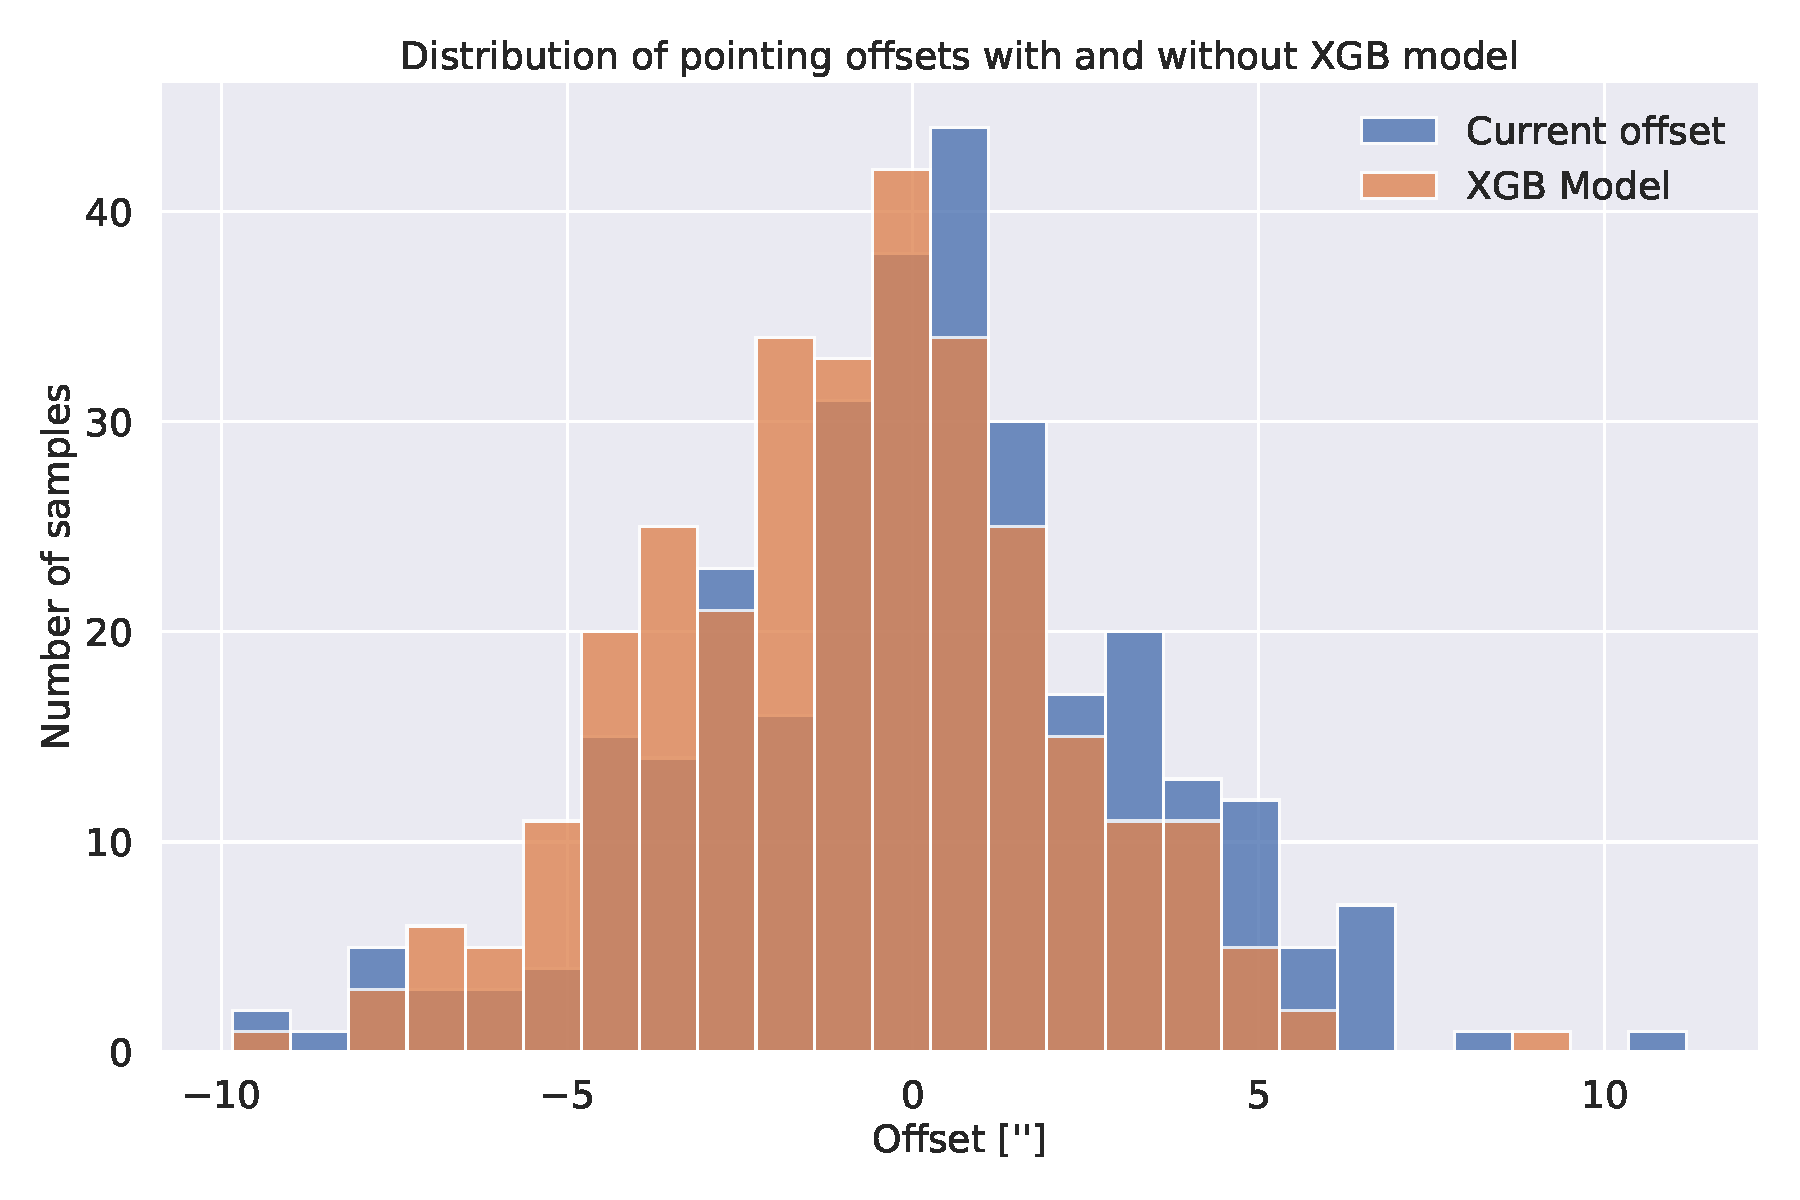
\includegraphics[width=\textwidth]{Results/hist_XGB_ds2_tp5_k30_uncorr_az_test.pdf}
        \caption{The azimuth model, with offsets reduced on the unseen test set by $7.0\%$.}
        \label{subfig:hist_lastfold_nflash230_az}
    \end{subfigure}
    \\
    \begin{subfigure}[t]{\textwidth}
       \centering
       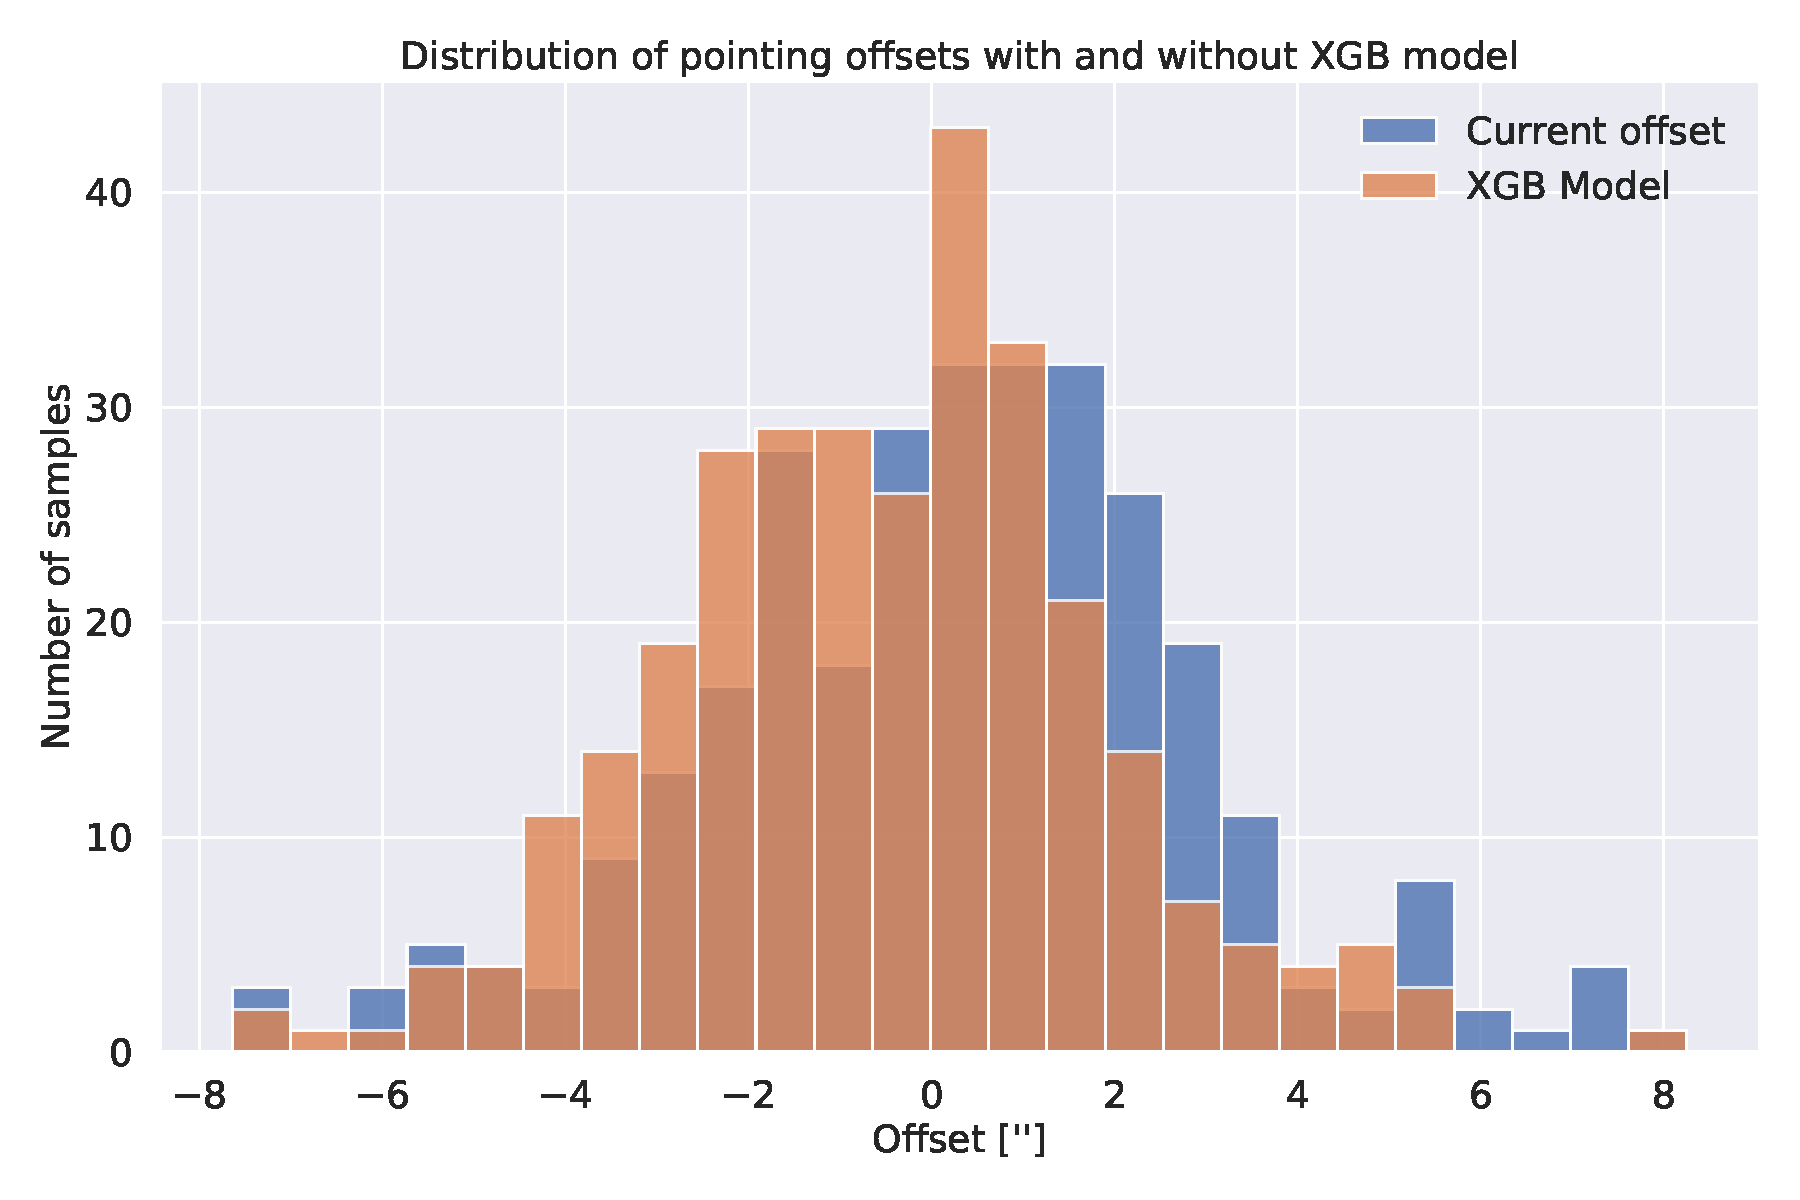
\includegraphics[width=\textwidth]{Results/hist_XGB_ds2_tp5_k40_uncorr_el_test.pdf}
       \caption{The elevation model, with offsets reduced on the unseen test set by $9.4\%$.}
       \label{subfig:hist_lastfold_nflash230_el}
    \end{subfigure}
    \caption[Offset distribution with and without pointing correction model]{Distribution of offsets with and without the NFLASH230 pointing correction model on the unseen test set for the last fold. \textbf{a)} Azimuth model and \textbf{b)} elevation model.}
    \label{fig:histogram_selected_result_xgb}
\end{figure}


Figure \ref{fig:sortpred_selected_result_xgb} show the predicted and observed pointing NFLASH230 offsets for all samples in the unseen test set of the last fold.
We sorted the samples by the true value in ascending order.


\begin{figure}[H]
    \centering
    \begin{subfigure}[t]{\textwidth}
        \centering
        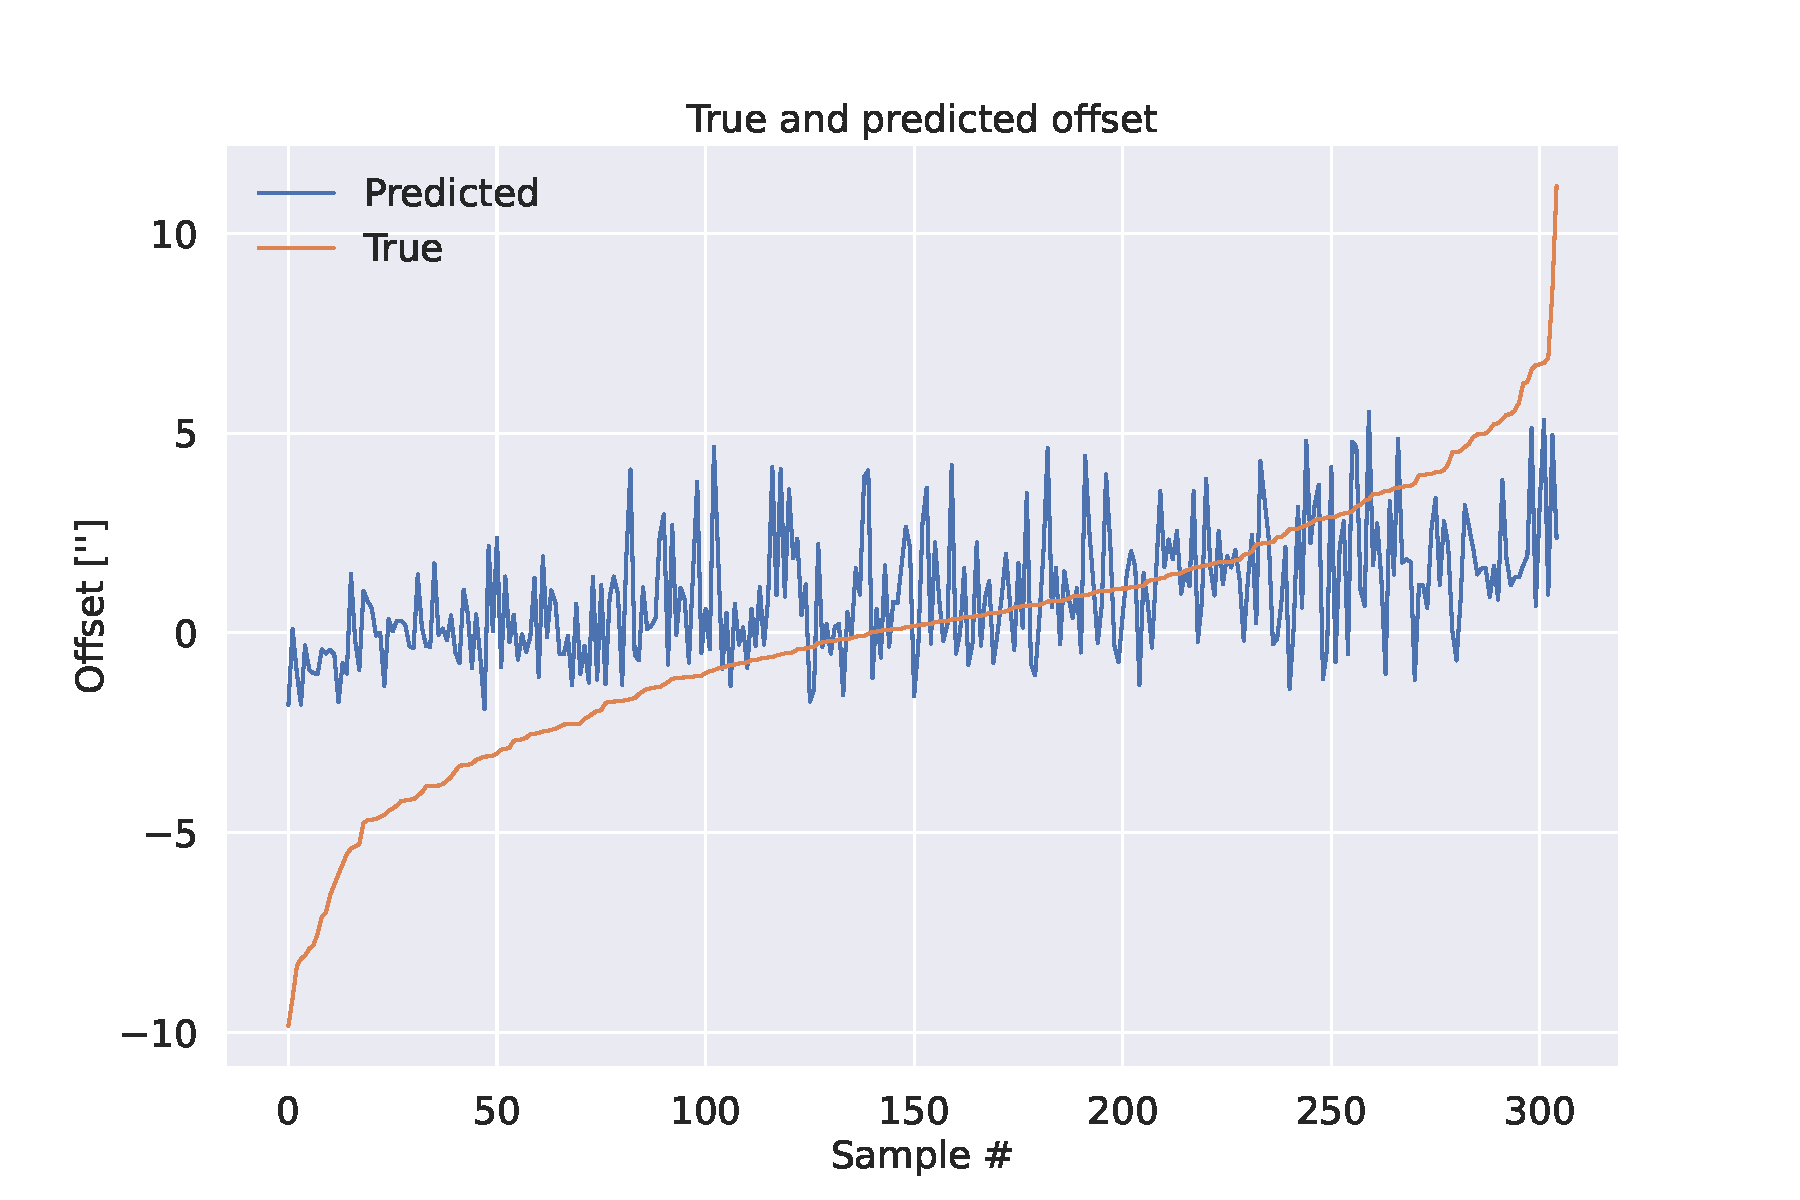
\includegraphics[width=\textwidth]{Results/sortpred_XGB_ds2_tp5_k30_uncorr_az_test.pdf}
        \caption{The azimuth model, with offsets reduced on the unseen test set by $7.0\%$.}
        \label{subfig:sortpred_lastfold_nflash230_az}
    \end{subfigure}
    \\
    \begin{subfigure}[t]{\textwidth}
       \centering
       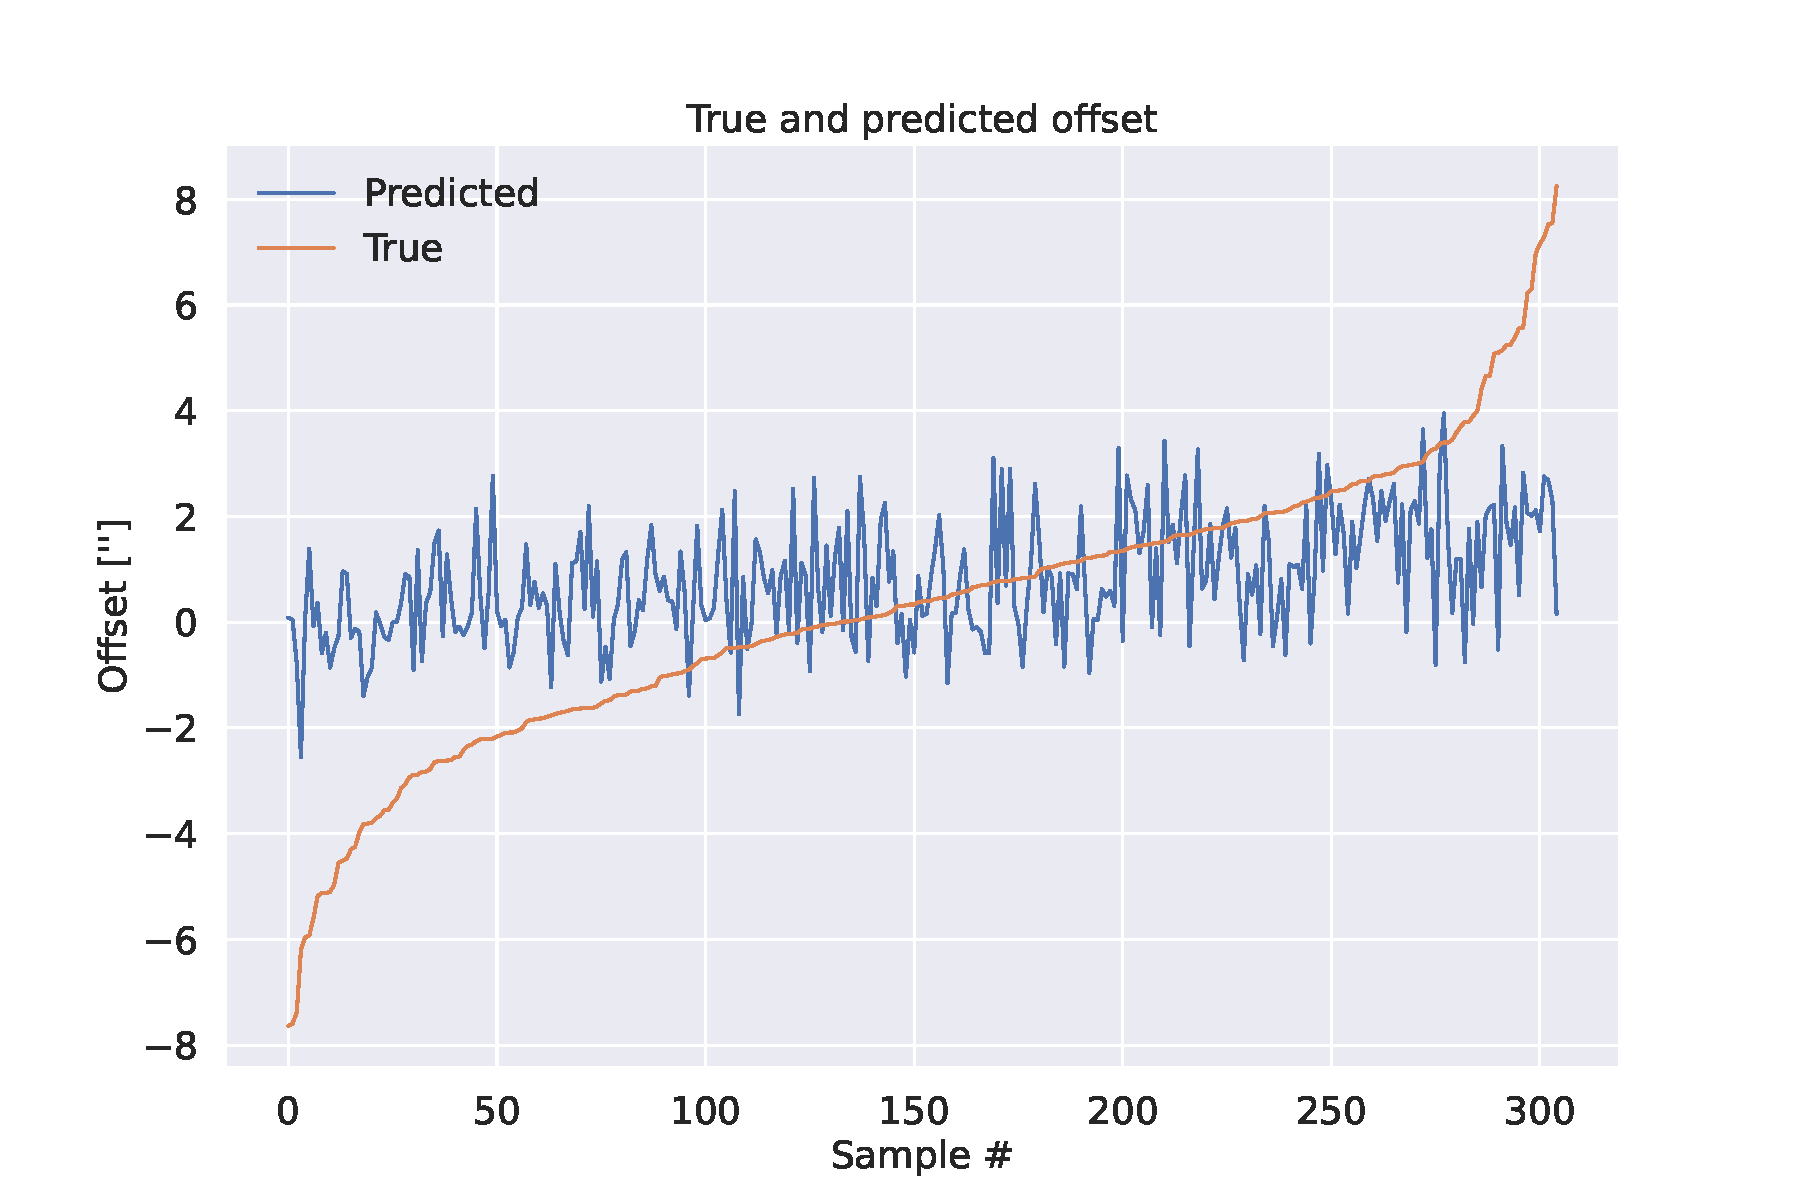
\includegraphics[width=1\textwidth]{Results/sortpred_XGB_ds2_tp5_k40_uncorr_el_test.pdf}
       \caption{The elevation model, with offsets reduced on the unseen test set by $9.4\%$.}
       \label{subfig:sortpred_lastfold_nflash230_el}
    \end{subfigure}
    \caption[Sorted offset prediction and true values]{Offset predictions by the NFLASH230 pointing correction model on the unseen test set for the last fold.
     Predicted and observed values, sorted in ascending order by observed value. \textbf{a)} Azimuth model and \textbf{b)} elevation model.}
    \label{fig:sortpred_selected_result_xgb}
\end{figure}



Figure \ref{fig:sage_lastfold_nflash230_az} show the SAGE values for the NFLASH230 azimuth pointing correction model on the validation set (Figure \ref{subfig:sage_lastfold_nflash230_az_val})
and test set (Figure \ref{subfig:sage_lastfold_nflash230_az_test}).
The same plots for the elevation models are presented in Figure \ref{fig:sage_lastfold_nflash230_el}.

\begin{figure}[H]
    \centering
    \begin{subfigure}[t]{0.92\textwidth}
        \centering
        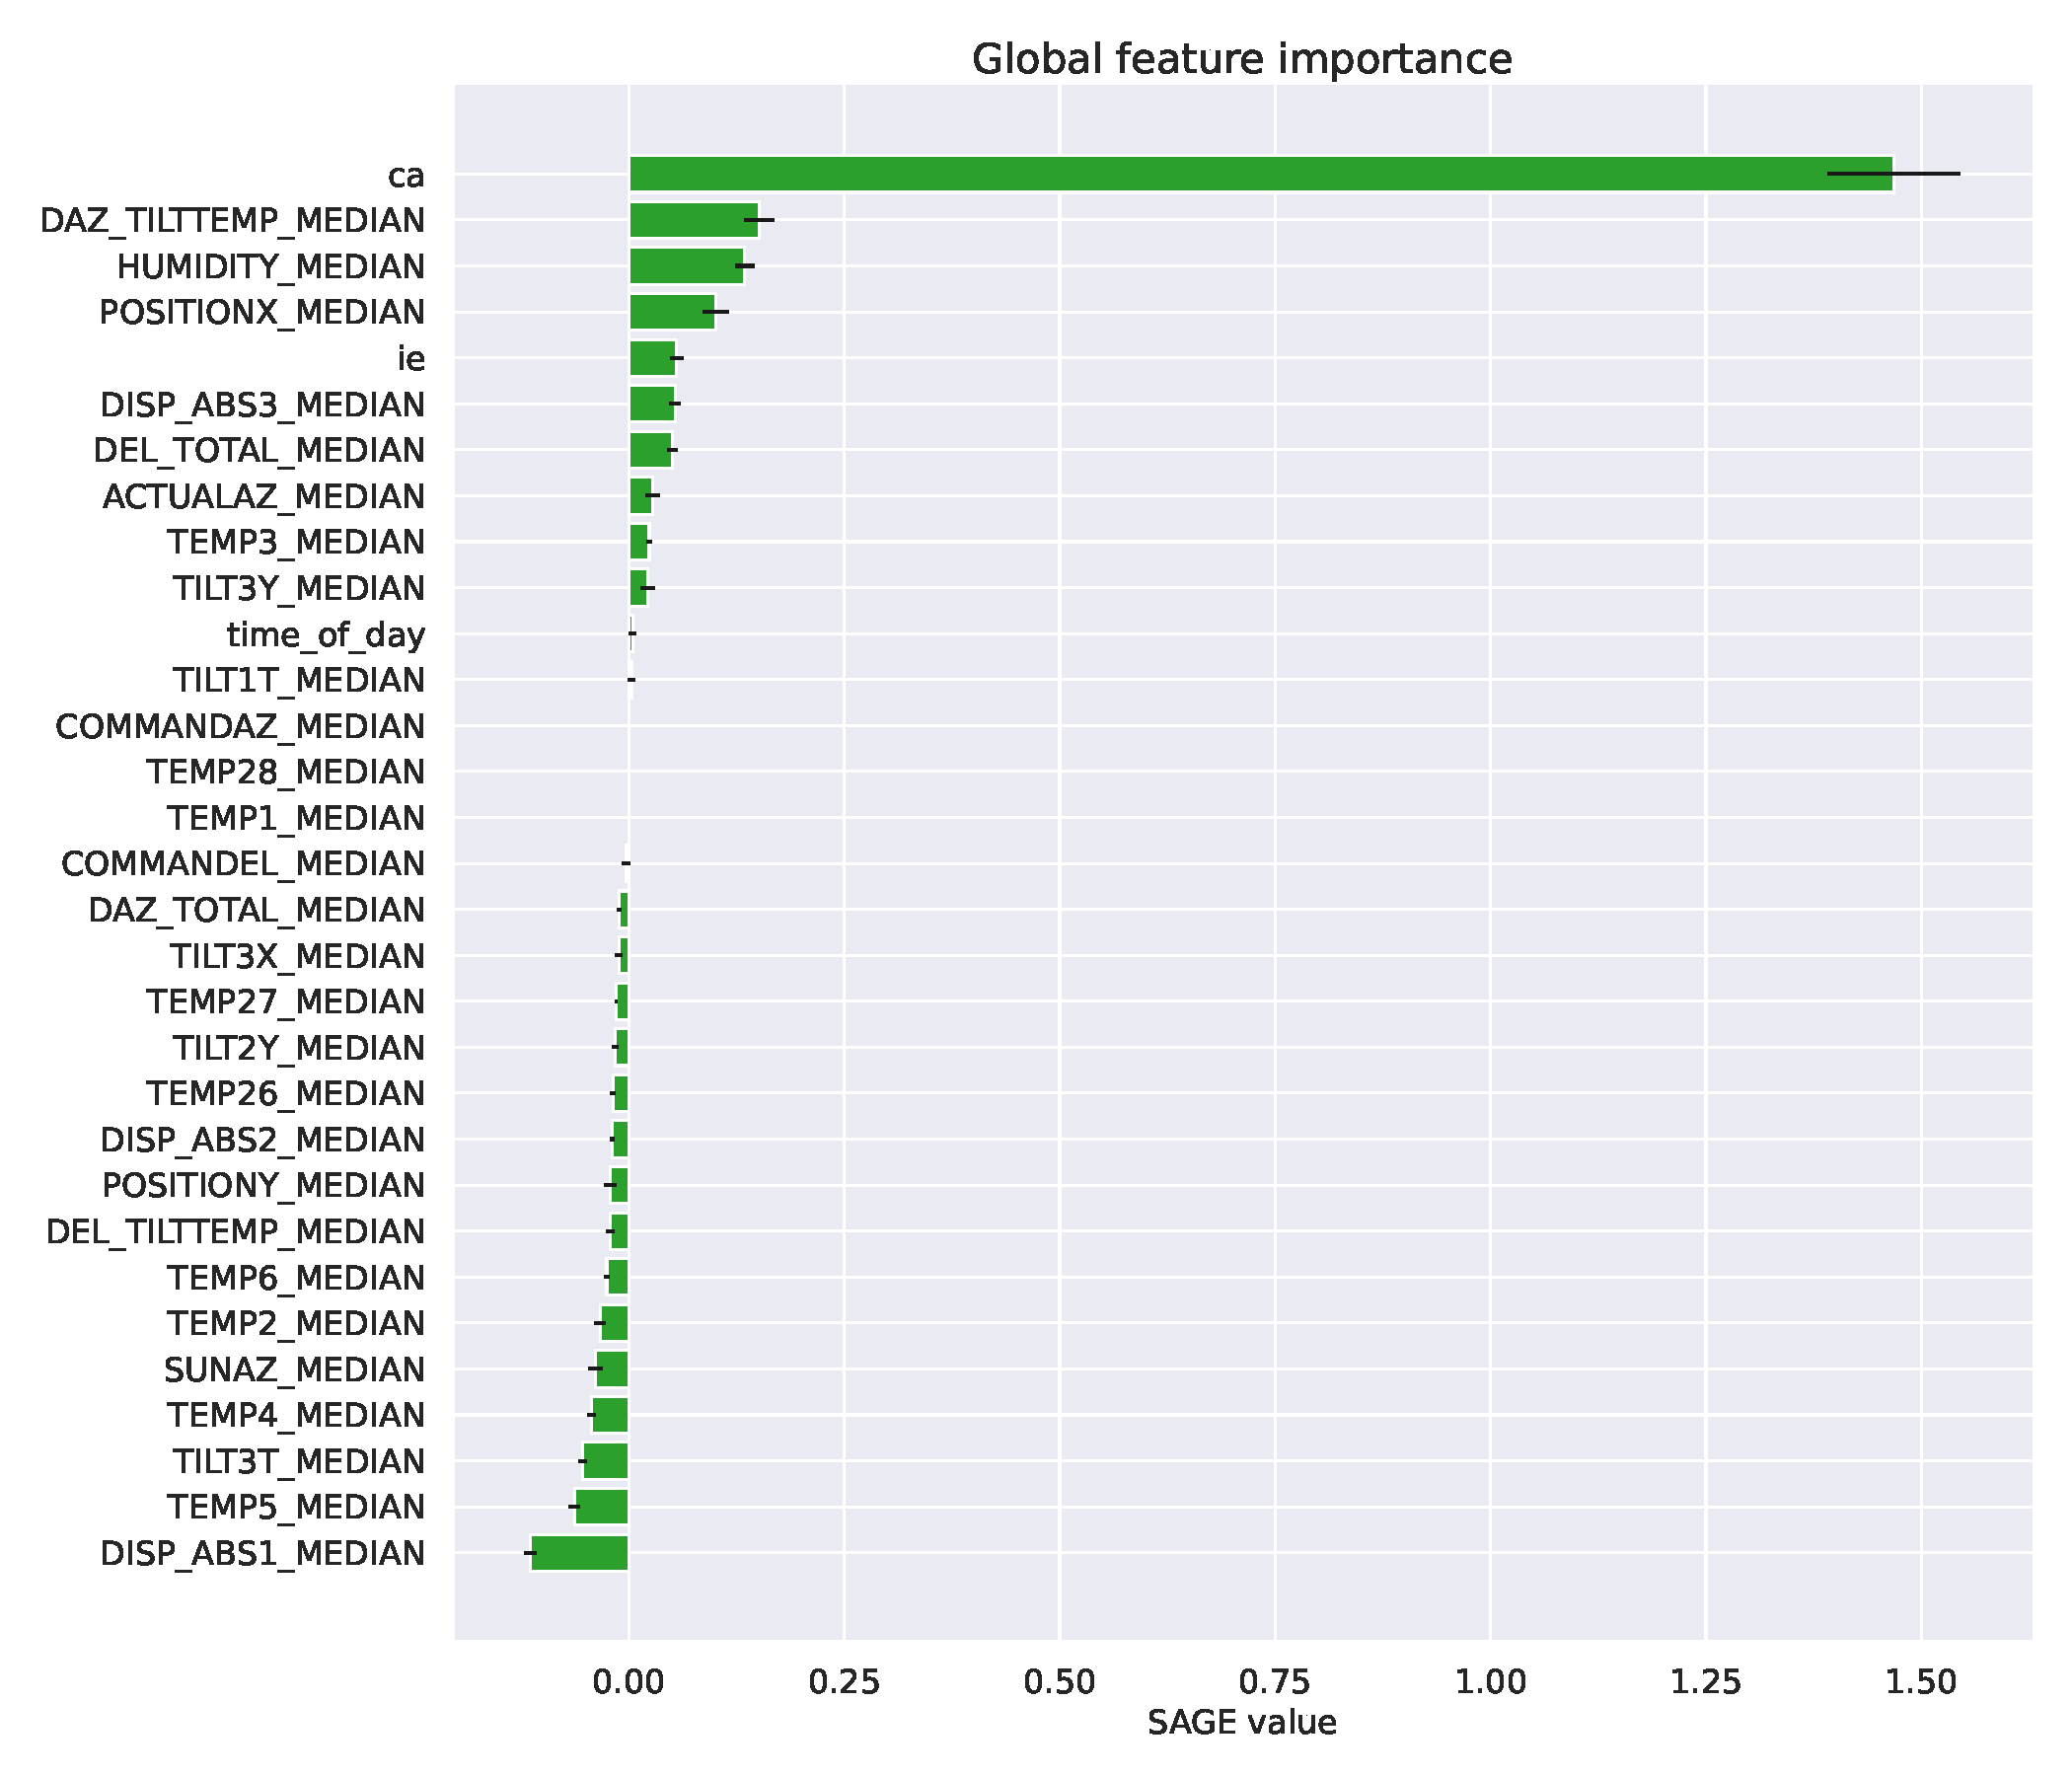
\includegraphics[width=\textwidth]{Results/XGB_ds2_tp5_k30_uncorr_az_val_SAGE.pdf}
        \caption{Validation set}
        \label{subfig:sage_lastfold_nflash230_az_val}
    \end{subfigure}
    \\
    \begin{subfigure}[t]{0.92\textwidth}
       \centering
       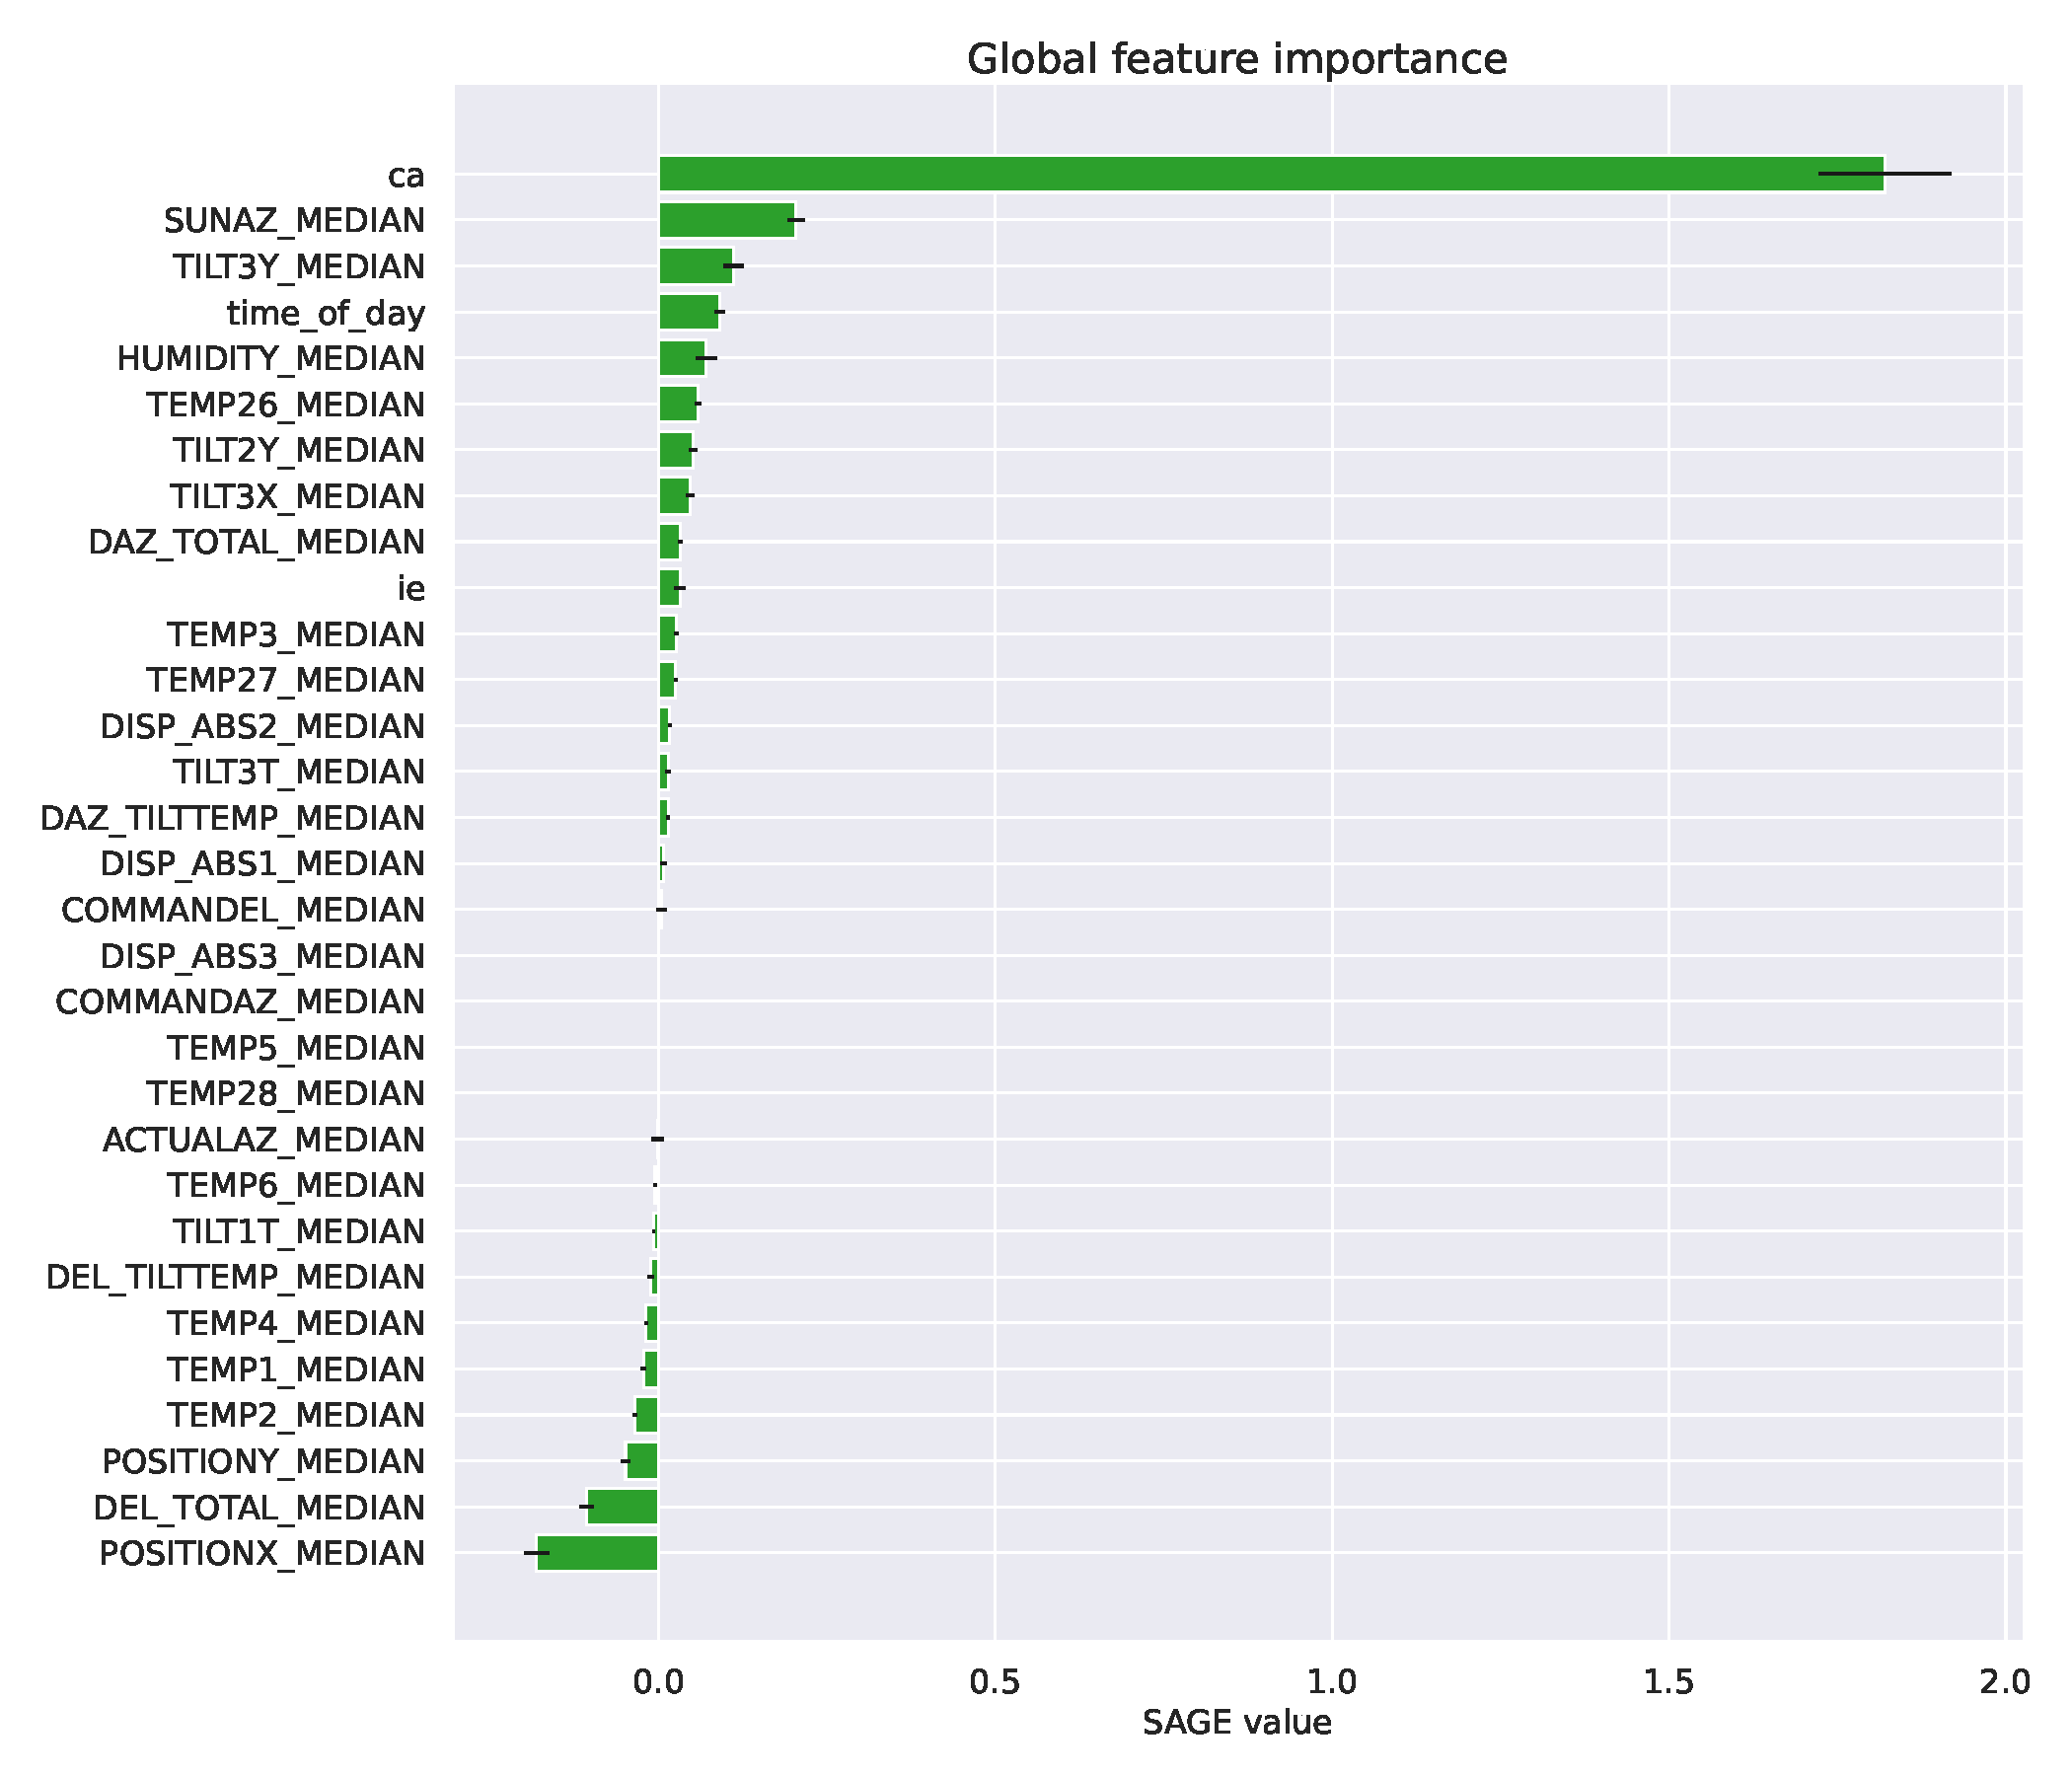
\includegraphics[width=1\textwidth]{Results/XGB_ds2_tp5_k30_uncorr_az_test_SAGE.pdf}
       \caption{Test set}
       \label{subfig:sage_lastfold_nflash230_az_test}
    \end{subfigure}
    \caption[SAGE values for NFLASH230 elevation pointing correction model]{SAGE values for the NFLASH230 azimuth pointing correction model on the a) validation set, and b) test set.}
    \label{fig:sage_lastfold_nflash230_az}
\end{figure}

\begin{figure}[H]
    \centering
    \begin{subfigure}[t]{0.92\textwidth}
        \centering
        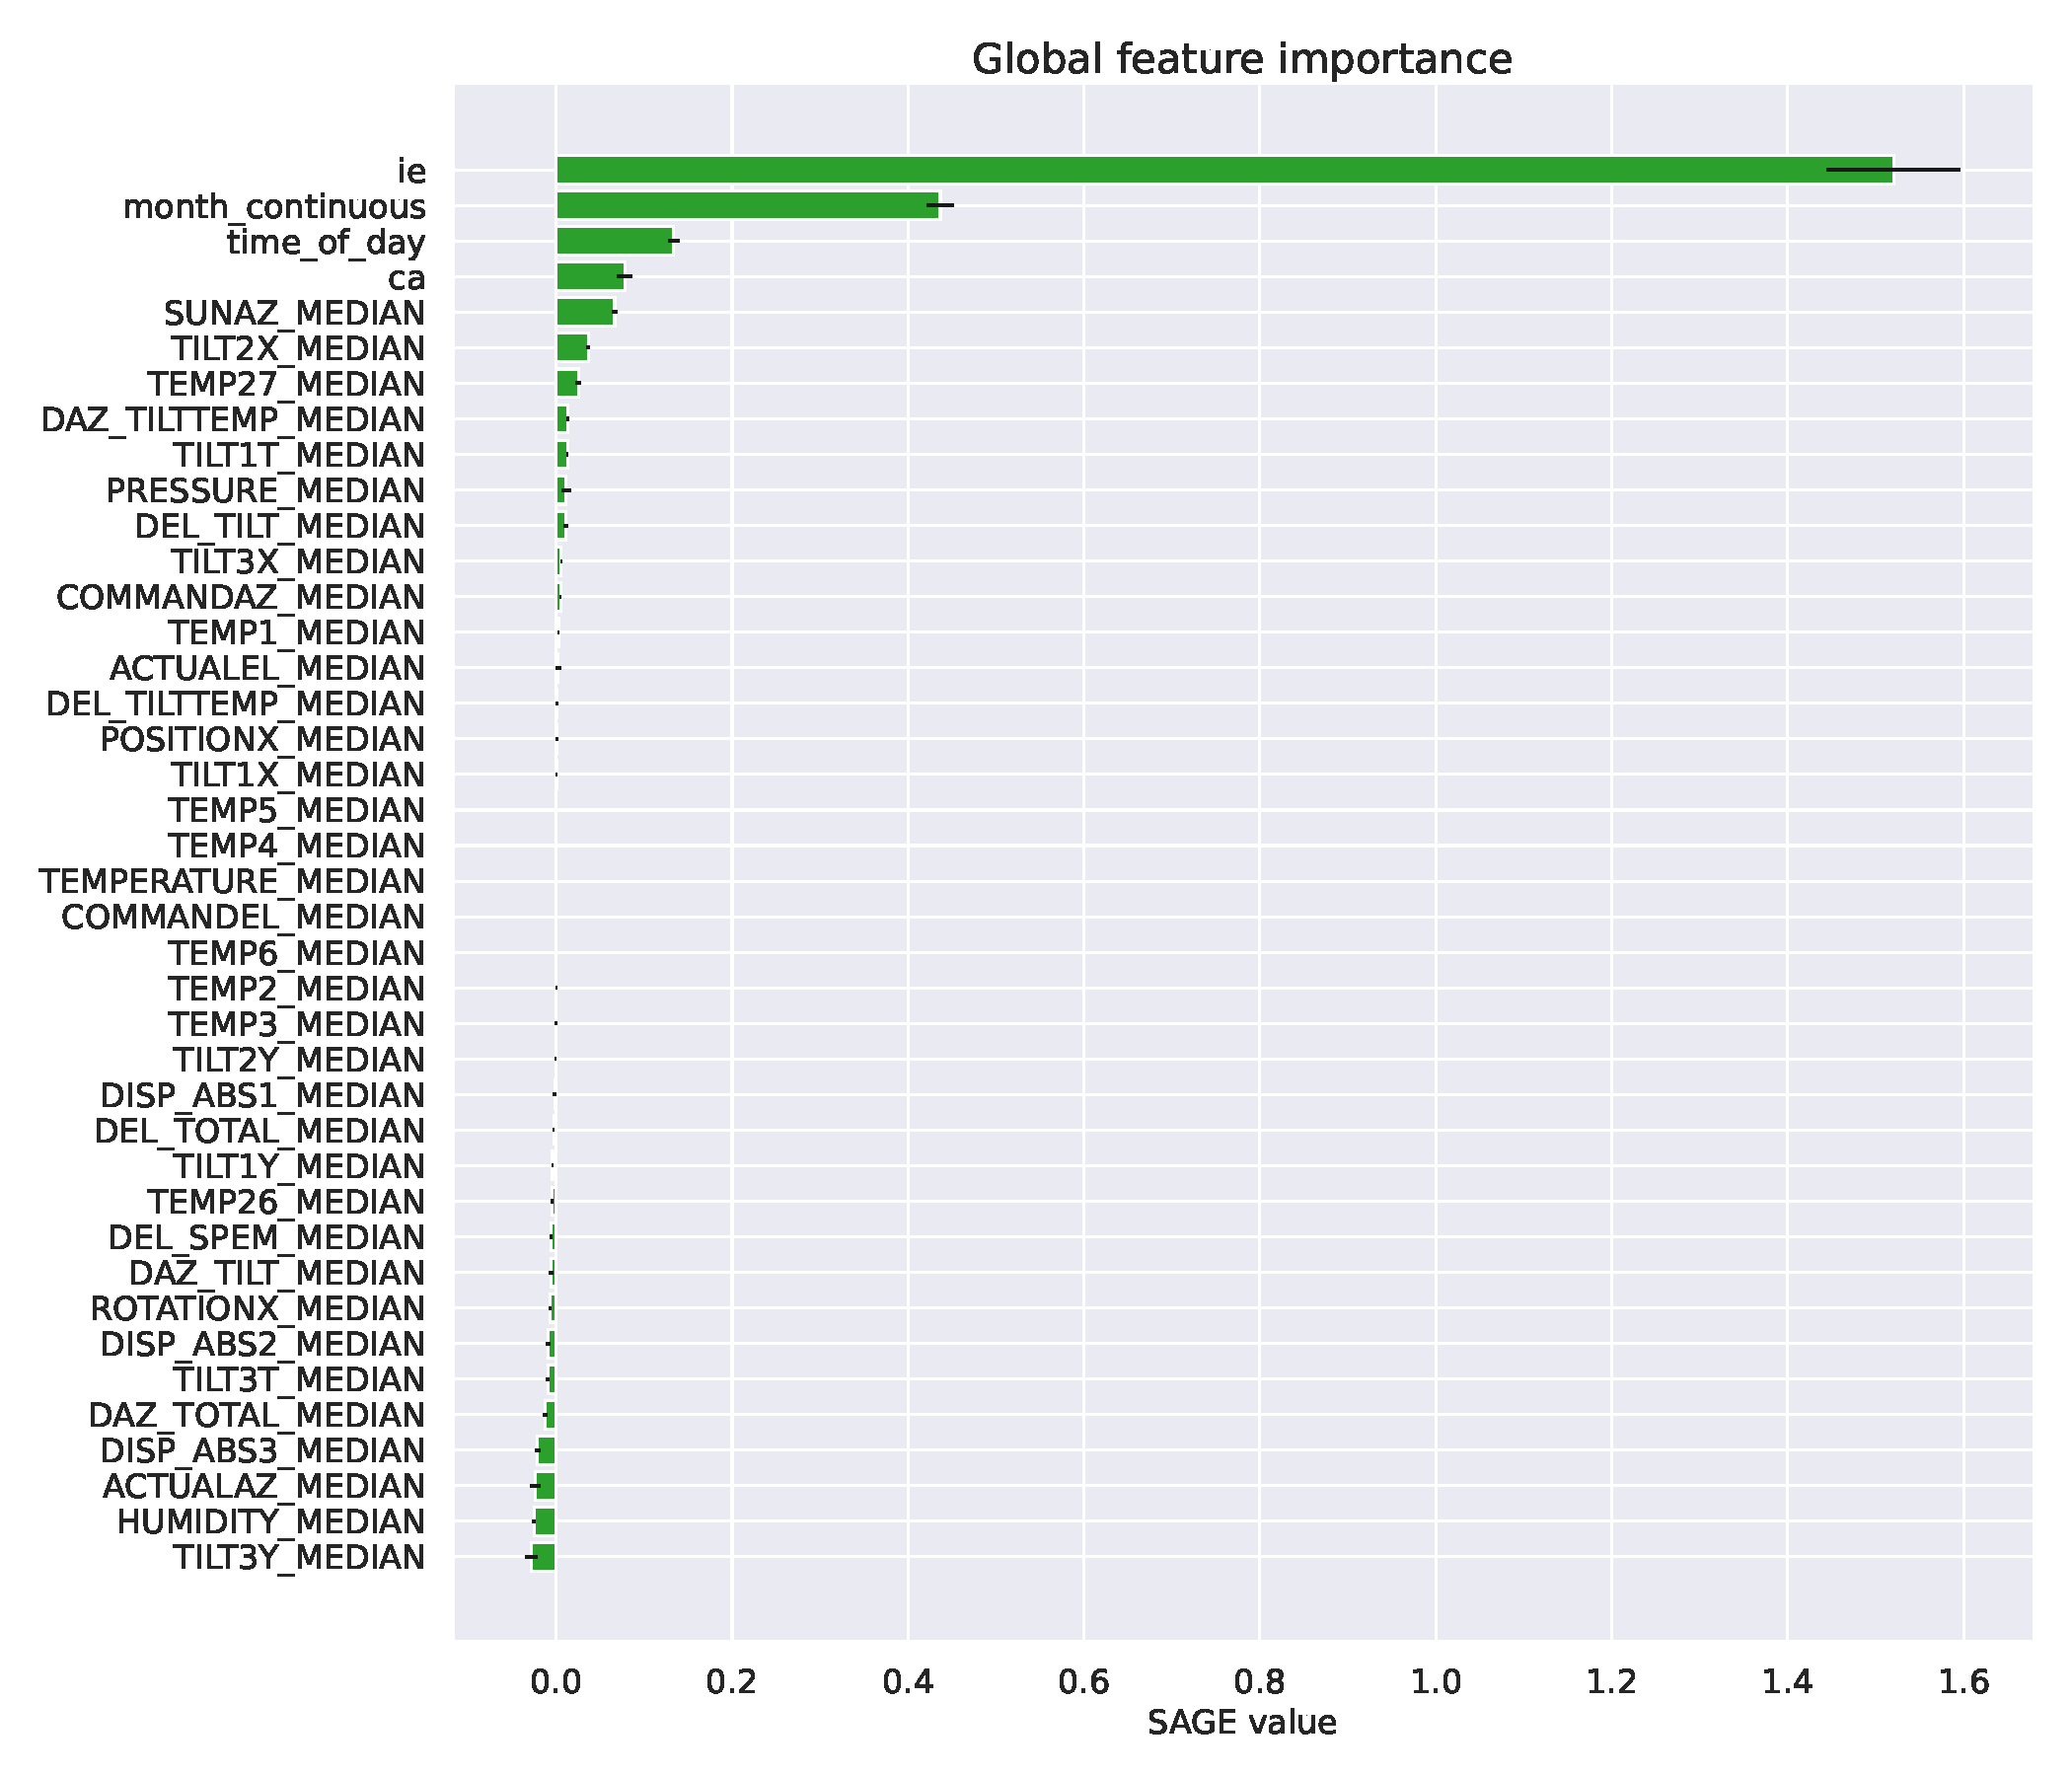
\includegraphics[width=\textwidth]{Results/XGB_ds2_tp5_k40_uncorr_el_val_SAGE.pdf}
        \caption{Validation set}
        \label{subfig:sage_lastfold_nflash230_el_val}
    \end{subfigure}
    \\
    \begin{subfigure}[t]{0.92\textwidth}
       \centering
       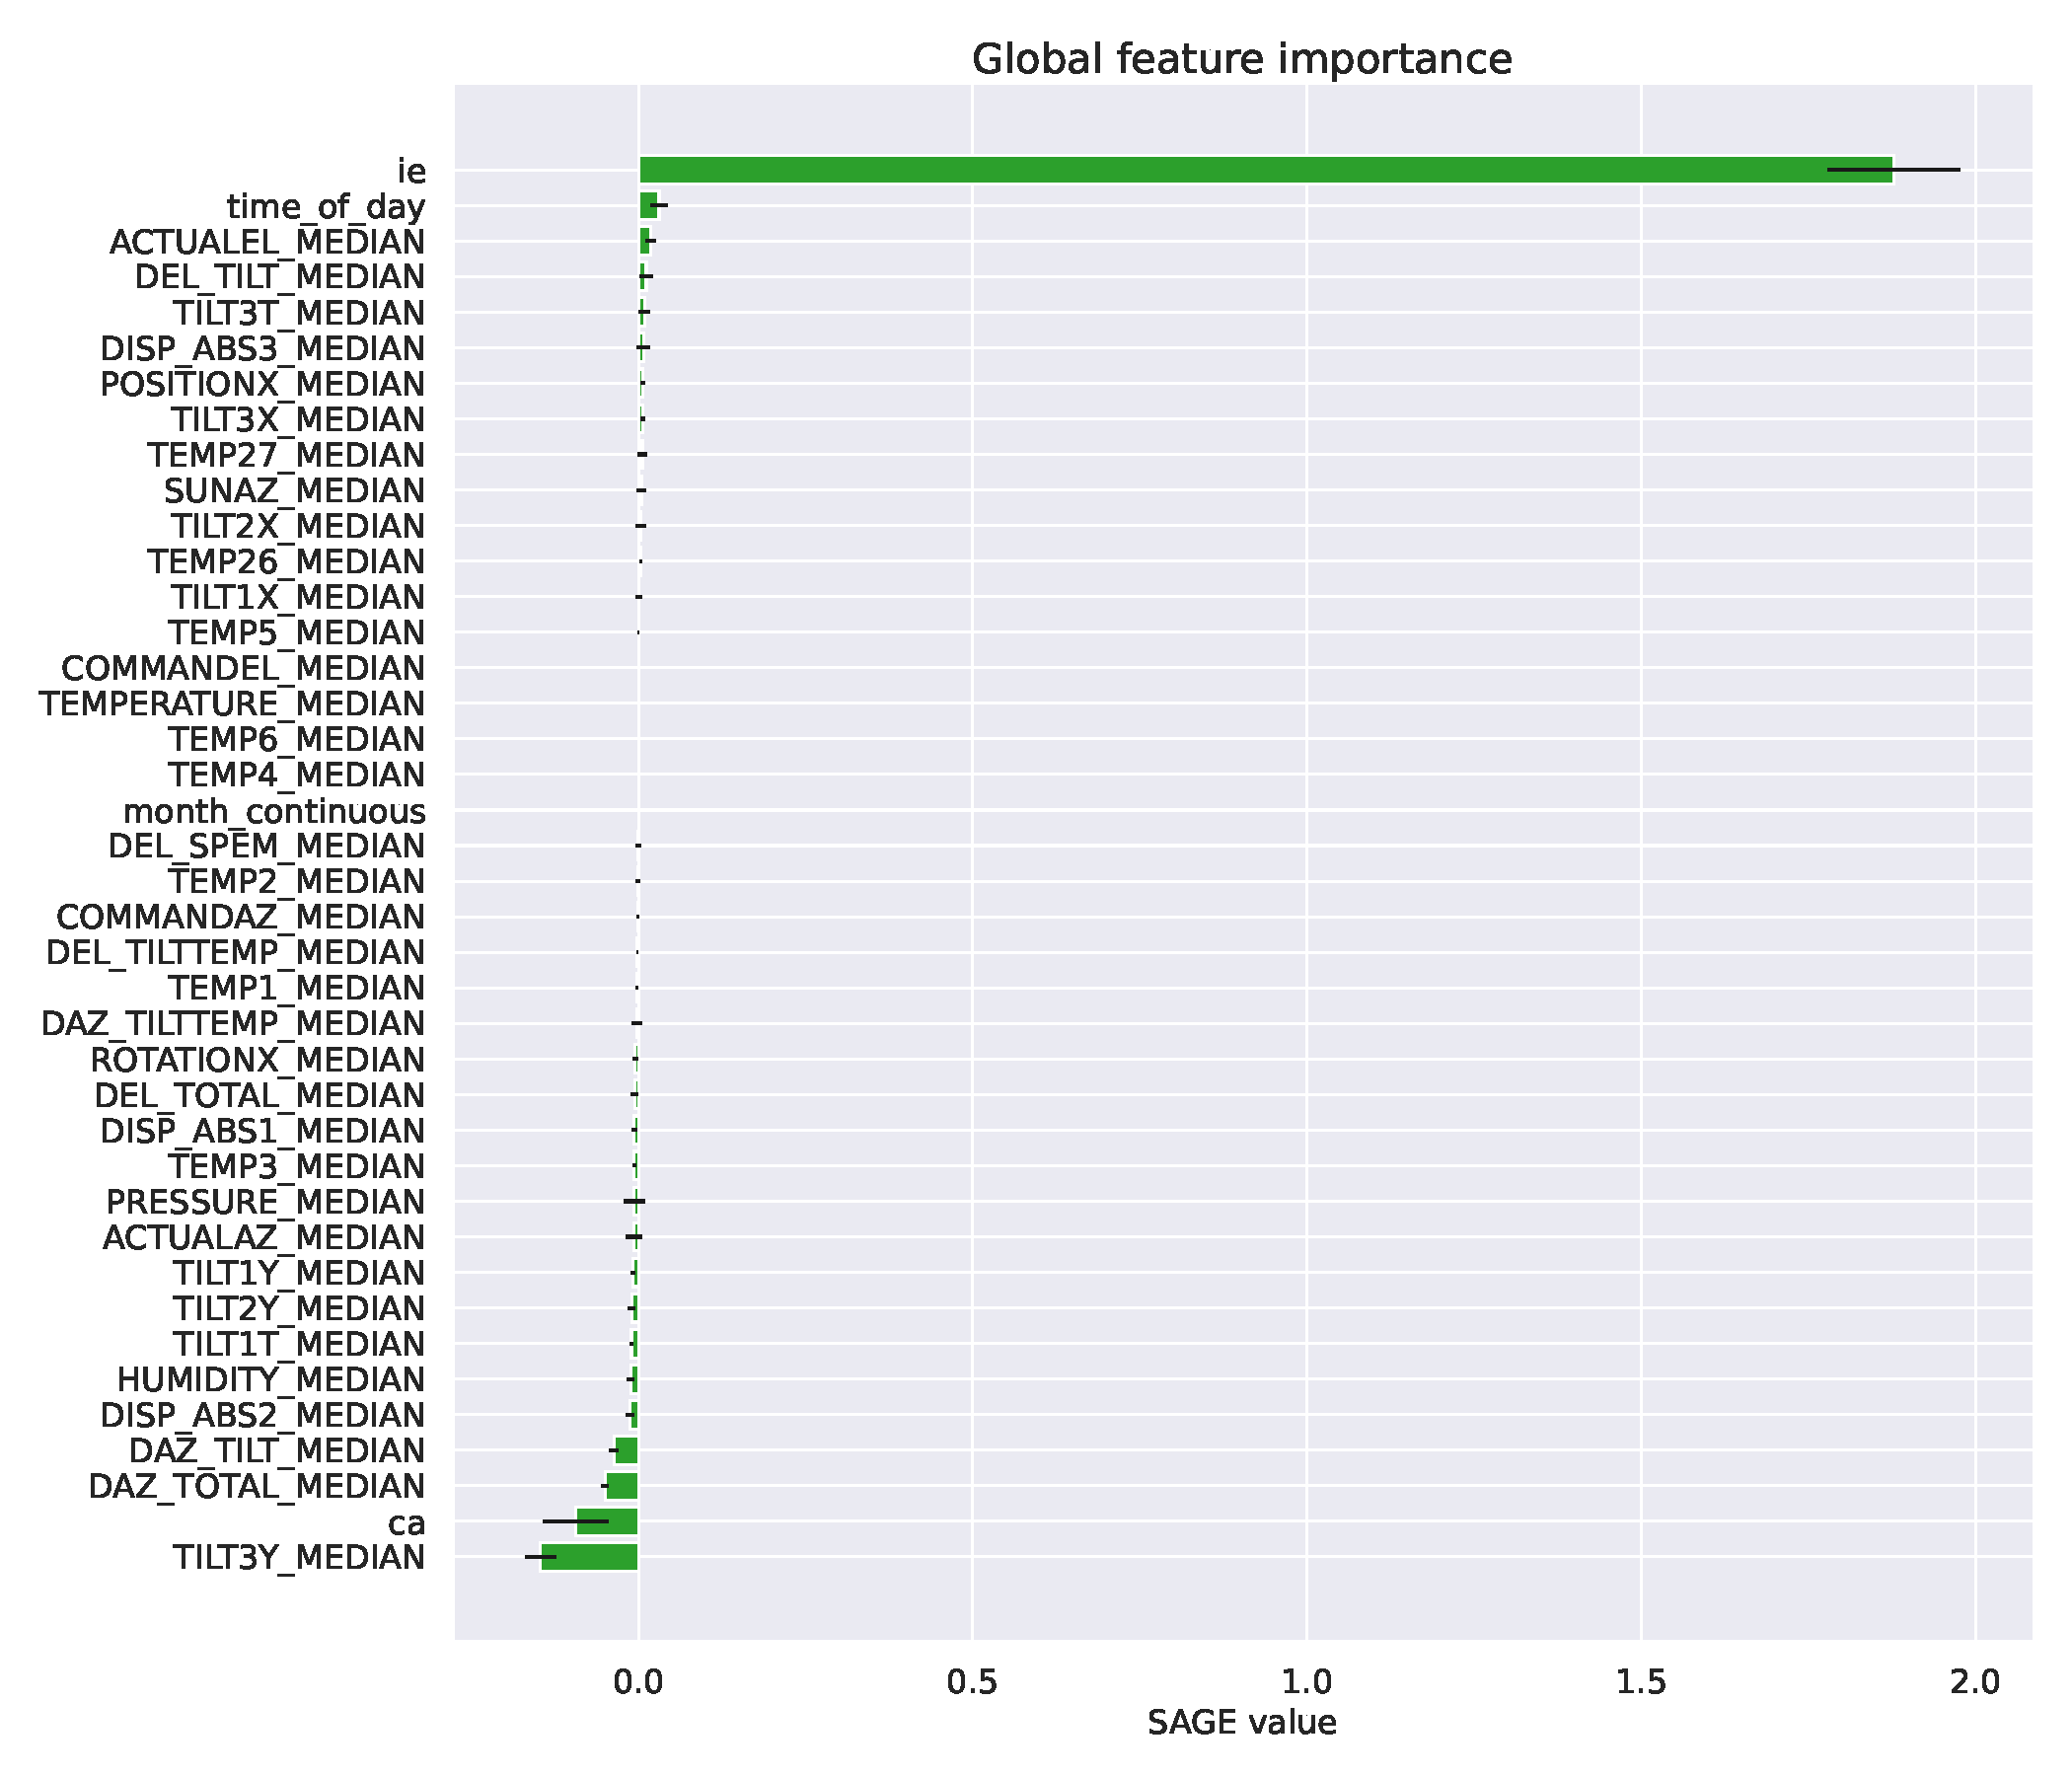
\includegraphics[width=1\textwidth]{Results/XGB_ds2_tp5_k40_uncorr_el_test_SAGE.pdf}
       \caption{Test set}
       \label{subfig:sage_lastfold_nflash230_el_test}
    \end{subfigure}
    \caption[SAGE values for NFLASH230 elevation pointing correction model]{SAGE values for the NFLASH230 elevation pointing correction model on the \textbf{a)} validation set, and \textbf{b)} test set.}
    \label{fig:sage_lastfold_nflash230_el}
\end{figure}


\section{Discussion of Experiment 1: Pointing Correction Model}
The first research question addressed in this thesis is whether machine learning can enhance the pointing accuracy of a radio telescope using the current pointing strategy.
To investigate this question, we explore a realistic scenario (case 1) in which a model is trained on a smaller period of data and used to predict the offset of consecutive scans for a period afterward.
We focus now on the model predicting the offsets of only NFLASH230.
The results from this case, presented in Table \ref{tab:results_minval_val_test_days_04_n230}, demonstrate that the model's performance on the validation set is promising,
with the root-mean-square (RMS) ratio in the range of approximately $0.80$-$0.85$ for azimuth and elevation,
which corresponds to a $15$-$20\%$ reduction in pointing offset.
However, this performance does not transfer to the following test period,
in which the RMS ratios are $1.16$-$1.46$, indicating a $16$-$46\%$ increase in pointing offset.
There are several possible reasons for the model's poor performance on the test set.
One of the limitations of tree-based models, such as XGBoost, is that they typically do not generalize well to new data that is different from the training data,
as they predict solely based on logical conditions seen in the training set.
If the factors affecting the pointing offset change over time and the new data is very different from the training data, the model will likely perform poorly. 
Furthermore, another potential explanation for the poor performance could be that the dataset is too small, and the model overfits on the validation set.
The results of this experiment suggest that learning the relationships in the data that affect pointing offset is challenging, and a complex model may be necessary.
To train a proper complex model, a larger amount of data is required, at least more than the number of samples in the training and validation sets for case 1.
The findings also indicate that choosing the complexity of the model with the best performance on the validation set may not necessarily lead to the best performance on the test set.
We further explore this aspect by examining Table \ref{tab:results_nflash_days}, which demonstrates the mean RMS ratio on the test set using the same number of features for all the folds.
This provides an idea of the complexity that might provide the best-performing models on the test set.
Even though the model with the best performance on the validation set is not chosen, which could be a lucky or overfitted performance,
no improvement is observed in the current pointing model on the test set.
However, the results show better performance than the first Table \ref{tab:results_minval_val_test_days_04_n230}.
The same trends are observed when predicting offsets from all instruments in Tables \ref{tab:results_minval_val_test_days_04_all} and \ref{tab:results_all_days}. \\


Moving on to case 2, which tests whether the amount of data is a limitation for enhancing the pointing accuracy.
In this case we split the data into six folds and performed cross-validation.
Since the training/validation data is either before or in between the test data in time (except for the last fold), this is a less realistic test case.
Results from this case indicate that a larger time period helps the model generalize better, which we expected as a longer period includes more variation that can help the model capture the relationships between features.
We start by looking at Table \ref{tab:results_minval_val_test_days_04_n230}.
Here, we also see a good performance on the validation set across all folds, with a $9$-$20\%$ reduced pointing offset on the validation set.
The average RMS ratio on all folds on the test set for case 2 is $0.958$ for azimuth and $0.941$ for elevation.
With the standard deviations, the $95\%$ confidence intervals would be put at $[0.850, 1.066]$ for azimuth and $[0.786, 1.010]$ for elevation.
Given that the upper bound of both confidence intervals is larger than one and the testing case is not realistic, we cannot conclude that the model can reduce the pointing offset robustly and consistently.
For an unbiased result that reflects expected performance in practice, we look at the RMS ratio for the last fold in Table \ref{tab:results_minval_val_test_days_04_n230},
showing a $7.0\%$ and $9.4\%$ reduced RMS for azimuth and elevation, respectively.
These results are the ones visualized in the histograms and plots in Figures \ref{fig:histogram_selected_result_xgb} and \ref{fig:sortpred_selected_result_xgb}, respectively.
It is not apparent from the histogram with the azimuth model results that the model performs better than the current model.
What we can see, however, is a shift in offsets towards the left, indicating more negative offsets.
This is consistent with the sorted prediction plot \ref{subfig:sortpred_lastfold_nflash230_az}, which shows a bias towards positive predictions.
There also seem to be slightly less large negative offsets.
Looking at the elevation histogram (Figure \ref{subfig:hist_lastfold_nflash230_el} and sorted prediction plot (Figure \ref{subfig:sortpred_lastfold_nflash230_el}), we can make the same analysis.
The histogram shows a shift towards the left, and the sorted prediction plot shows a bias toward positive predictions.
We do also see that there are more offsets in the center bin in the histogram (meaning more smaller offsets).
The tails in the sorted prediction plots also seem steep, indicating that the cleaning could have been better.\\


We now discuss the results of the SAGE analysis on the validation and test sets for the NFLASH230 model on the last fold,
as shown in Figures \ref{fig:sage_lastfold_nflash230_az} and \ref{fig:sage_lastfold_nflash230_el}.
This analysis helps us understand the factors that improve and worsen the models' performance on unseen data, thereby providing insights into how the models can be improved.

For the azimuth model, we observe that the azimuth correction $ca$ is the most important feature, contributing significantly to the model's performance on both the validation and test sets.
However, the elevation correction $ie$ shows a mixed effect on the model's performance.
While it improves the performance on the validation set, it worsens the performance on the test set.
This indicates that there are some correlation between the azimuth and elevation correction that change over time.
% Surprisingly, some features such as the azimuth angle of the sun and the $X$ position of the subreflector (POSITIONX) worsen the performance on the validation set, but improve it on the test set.
% We do not have a clear explanation for this behavior.
Notably, the COMMANDAZ and COMMANDEL features, which are included in every model, do not affect the azimuth or elevation model's performance.
This suggests that the analytical pointing model, which is based solely on azimuth and elevation, is performing very well, and the offsets are likely attributed to factors other than the pointing direction.
We also find that the continuous month feature is the second most important feature in the elevation model, after the elevation correction $ie$.
However, the model's performance on the test set does not benefit from this feature, as its value is larger in the test set than in the training and validation sets.
This is one of the weaknesses of tree-based models.
Training the model on the previous years' data could solve this problem, as long as there are no other significant changes in the structure or mounting of the instruments.

% We now look at the results from the SAGE analysis on the validation and test set, shown in Figures \ref{fig:sage_lastfold_nflash230_az} and \ref{fig:sage_lastfold_nflash230_el},
% for the same model we discussed in the previous paragraph.
% Analyzing which features improve and worsen the performance on unseen data is a good way of understanding what makes the model better and worse.
% We start by looking at the sage values for the azimuth model \ref{fig:sage_lastfold_nflash230_az}.
% It shows that the azimuth correction $ca$ applied during the given pointing scan stands for most of the good predictions on both the validation and test set.
% The elevation correction $ie$ improves the performance on the validation set, but worsen the performance on new data.
% Interestingly enough, there are features like the azimuth angle of the sun and x position of the subreflector that makes the performance on the validation set worse, but improve the performance on the test set.
% We cannot explain this behavior either.
% Interestingly enough, COMMANDAZ and COMMANDEL, which is incorporated in every model, does not affect the performance of the model at all.
% This indicates that the analytical pointing model, which is only based on azimuth and elevation, is performing very well,
% and the reasons for the offsets are attributed to other factors.
% One interesting note, is that the continuous month feature in the elevation model is the second most important feature, after the elevation fcorrection $ie$.
% However, on the test set, the month continuous variable does not help the model at all.
% This is very expected behavior, as this value is larger on all the pointing scans in the test set, and therefore it cannot help the model,
% as there is nothing trained on the month being larger than it is in the training and validation set.
% Again here, we see taht the input coordinates are of no use for the model.



In summary of the results from case 2, we see promising results with machine learning models further reducing the offsets slightly.  
This indicates that a possible pointing strategy could be training a model on multiple months worth of data and then using the model for a couple of weeks.
An even better strategy could be training on previous years' data.
However, given the limited data available in this project, this could not be tested thoroughly.
If more data were available,
we could preform a similar analysis with the start and end time of both the train/validation and test set moved by two weeks and iteratively train new models to predict the offsets for the next period in time.
This could verify whether the improved performance repeats.\\



In case 2, the model predicting offsets from all instruments shows results similar to the model predicting only NFLASH230 offsets, though with slightly worse performance.
The reduced performance is likely due to less training data available for the other instruments.
The difference in performance between these two models provides some insights.
First, it suggests that various factors influence the different instruments differently.
Otherwise, we expect the larger model to perform better than the smaller model.
The reason that each instrument can be affected differently is because of the different mounting locations at the telescope.
Different mounting locations mean that the path of photons leading to the receiver can vary, leading to distinct factors affecting the pointing.\\


There are several measures we could take to enhance the analysis further. One such measure is to improve feature engineering.
When the quantity of training data is limited, it is vital to ensure that the features are as informative as possible.
For example, instead of including six distinct temperature measurements in a model,
it may be preferable to create terms based on the difference between multiple temperature measurements, as they did in \cite{whitegreen2022}.

Another step is to integrate corrections for $ca$ and $ie$ into the offset that we intend to predict.
These corrections are applied at each pointing scan and display the strongest correlation to the target offset of all the features,
and we therefore incorporated them in all the models.
By transforming the offsets $\delta_{az}=\delta_{az} + ca$ and $\delta_{el}=\delta_{el} + ie$, we can then eliminate $ca$ and $ie$ from the input to the models.
This could remove a layer of complexity for the model.\\


Another option to consider for predicting the pointing offsets is to use neural networks.
These models offer several advantages if trained successfully.
For instance, they can handle multiple outputs and thus only require a single model.
By training the neural network with two outputs, it can simultaneously consider the offsets in azimuth and elevation and explore the correlation between them.
It would also be beneficial to fine-tune the network as new pointing scans become available continuously.
Despite their potential benefits, our initial tests with neural networks did not yield satisfactory results,
likely due to the limited training data available. Neural networks also require more tuning, which makes them more difficult to use with limited datasets.\\


To further improve the analysis, there are other possible areas for exploration, such as minimizing the number of pointing scans conducted by the astronomers.
While performing scans every one to two hours is standard practice, this can be time-consuming and may disrupt science observations.
A possible approach to investigate this possibility is to identify periods when pointing scans are conducted every hour or so.
Rather than providing the model with the corrections $ca$ and $ie$ obtained following the previous pointing scan,
the model can use the corrections from a pointing scan six hours earlier as inputs to evaluate the performance.
In this case, reducing pointing offsets is not a primary objective of the machine learning approach.
Instead, maintaining the same level of pointing accuracy while conducting fewer pointing scans would be a satisfactory outcome.\\



% \begin{itemize}
%     \item comment on parameters
%     \item discuss the adjustments made by system,a nd that the analytical poinitng models change over time too, which can make it harder for amodel, considering there are many other factors to ocnsider.
% \end{itemize}

% \section{Experiment 2: Pointing Correction Model}
% The first research question is if we can use machine learning to increase the pointing accuracy using the same pointing strategy as today.
% We start by discussing case 1, which test a realistic scenario of training a model on a smaller period,
% and then using the model to predict the offset of the consecutive scans for a period.
% We look first at the model using NFLASH230 data only.
% The results from this case show that the performance on the validation set is good \ref{tab:results_minval_val_test_days_04_n230},
% with the RMS ratio being in the range $\tilde{}0.80$-$0.85$ for azimuth and elevation.
% That corresponds to a $15$-$20\%$ reduced pointing offset.
% This performance does not transfer to the following test period,
% for which the RMS ratios are in the range $1.16$-$1.46$, corresponding to a $16$-$46\%$ increased pointing offset.
% There could be multiple reasons for the drastically worse performance set.
% One possibility is that the relationships learned by the model change over time, therefore the model is not able to perform well.
% This is one limitation of tree based models like XGBoost.
% Because the model is predicting solely on logical conditions seen in the training set,
% it is not able to generalize well to new data.
% A neural network could potentially perform better on unseen data, as it train a continuous function.
% Another reason is that the dataset is too small, and the performance on the validation set is based on luck.
% In other words, model overfits on the validation set.
% From this project, it is clear that learning the relationships in the data that affects the pointing offset is not easy, and a complex model might be essential.
% And in order to train a proper complex model, we need large amounts of data,
% at least more than the \textcolor{red}{train set num} and \textcolor{red}{train set num} samples in the training and validation set respectively.
% The resutls we just discussed, uses a strategy where we choose the complexity of the model with the best performance on the validation set.
% We now look at Table \ref{tab:results_nflash_days}, which shows the mean RMS ratio on the test set using the same number of features $k$ for all the folds.
% This gives an idea on what complexity could provide the best models.
% It shows that even though we do not choose the model with the best performance on the validation set, which could potentionally be a lucky performance or overfitted,
% we still do not see any improvement of the current pointing model on the test set.
% We do however see better results than in the first table \ref{tab:results_minval_val_test_days_04_n230}.
% If we look at the model using the data from all instruments, we see similar results \ref{tab:results_minval_val_test_days_04_all} \ref{tab:results_all_days}.\\

% Now onto case 2, which show a less realistic test case, but can give an idea on if the amount of data is a limitation.
% This test case is less realistic because we split the data into $6$ folds and perform cross validation.
% For all folds except for the last one, the test period will be either before, or between the training/validation set.
% Therefore, these results does not reflect expected performance in practise.
% We start by looking at the same table \ref{tab:results_minval_val_test_days_04_n230},
% with results from the NFLASH230 model choosing the best model from the validation set, and tests the performance on the test set.
% Again, we see a good performance on the validation set across all folds, with a $9$-$20\%$ reduced pointing offset, for azimuth and elevation models.
% Now, we also see a reduced pointing offset even on the test set.
% This shows that more training data helps the model generalize,
% which is somewhat expected considering that a larger time period includes more variation, which helps the model capture relations between features.
% The average RMS ratio on all folds for case 2 is $0.958$ for azimuth and $0.941$ for elevation.
% With the standard deviations, the $95\%$ confidence intervals would be put at $[0.850, 1.066]$ for azimuth and $[0.786, 1.010]$ for elevation.
% The results show that there is something to be learnt in the data, and this pointing strategy could potentially lead to improved pointing.
% For a completely unbiased result, which show a performance that could have been achieved in practice,
% we look at the RMS ratio for the last fold in Table \ref{tab:results_minval_val_test_days_04_n230}.
% This shows a $7.0\%$ and $9.4\%$ reduced RMS for azimuth and elevation respectively,
% which indicates that a possible pointing strategy could be training a model on multiple months worth of data, and then use the model for a couple of weeks.
% Given we only have six months of data, this could not be tested more thoroughly.
% If we had more data, we could trained a model on the same amount of data, but moving the start and end time of both the train/validation and test set by two weeks, and
% see if the improved performance repeats.




% \begin{align}
%     CI_{Az} &= \bar{r}_{RMS_Az} \pm 1.96 \cdot \sigma_Az = [0.958 - 1.96\cdot 0.055, 0.958 + 1.96\cdot 0.055] = [0.850, 1.066]  \\
%     CI_{El} &= \bar{r}_{RMS_El} \pm 1.96 \cdot \sigma_El = [0.941 - 1.96\cdot 0.079, 0.941 + 1.96\cdot 0.079] = [0.786, 1.010]
% \end{align}


\section{Results of Experiment 2: Pointing Model using Neural Networks}

Table \ref{tab:exp1_rms_folds_best_model} shows the RMS in arcseconds on the test set over all folds for the different model architectures.
The models presented in this table are the ones with the lowest mean RMS across all test folds.
A linear regression model is included for comparison. 
It is clear that neural network architectures significantly outperform the linear regression model.
The mean RMS over all folds show that the different neural network architectures offer similar performance.
We also see that the RMS of fold $1$ is far worse than the other folds.
The lowest mean RMS is from the architecture where the non-linear features are connected to the geometrical and harmonic features.\\

\begin{table}[!htbp]
    \centering
    \caption[RMS of each pointing model architecture on all test folds]{The RMS of the pointing model on the test set in each fold for all neural network architectures.
    The different architectures are described in Figure \ref{fig:nn_architecture}.}
    \begin{tabular}{lcccccccc}
        \toprule
        & \multicolumn{6}{c}{RMS [$''$] on test fold} & & \\
        \cmidrule(lr){2-7}
        Network & 1 & 2 & 3 & 4 & 5 & 6 & Mean & STD\\
        \midrule
        Regular           & 28.06 & 19.34 & 12.28 & 13.25 & 17.19 & 16.33 & 17.74 & 5.19 \\
        Separated 1       & 30.69 & 16.93 & 13.76 & 10.04 & 15.77 & 13.61 & 16.80 & 6.57 \\
        Separated 2       & 27.34 & 20.75 & 12.65 & 24.17 & 13.64 & 16.69 & 19.21 & 5.38 \\
        Separated 3       & 30.27 & 20.59 & 14.01 & 10.76 & 13.67 & 10.34 & 16.61 & 6.97 \\
        Linear regression & 70.55 & 40.19 & 51.17 & 49.69 & 36.86 & 37.29 & 47.63 & 12.81 \\
        \bottomrule
    \end{tabular}
    \label{tab:exp1_rms_folds_best_model}
\end{table}


Table \ref{tab:exp1_hyperparameters_best_model} shows the hyperparameter used for the best models.
All architectures perform better with a single hidden layer.
The regular neural network uses ReLU activation and MSE loss \eqref{eq:mse1}, while the other architectures use Tanh activation and MSD loss \eqref{eq:msd}.
The regular neural network also has more neurons in the hidden layer and a higher learning rate.
The batch size is also varying. There seem to be similarities between the hyperparameters chosen for the three architectures with separate features.
However, given the large standard deviation of the mean RMS, there are probably bigger issues than hyperparameter tuning.\\

\begin{table}[!htbp]
    \centering
    \caption[Selected hyperparameters for each neural network pointing model architecture]{Hyperparameters used in the best-performing model for each architecture.}
    \begin{tabular}{lccccc}
        \toprule
        Architecture & Activation & Hidden Layers & Learning Rate & Batch Size & Loss \\
        \midrule
        Regular &  ReLU & [82] & 0.0199 & 334 & MSE \\
        Sep1    &  Tanh & [40] & 0.0098 & 101 & MSD \\
        Sep2    &  Tanh & [40] & 0.0098 & 101 & MSD \\
        Sep3    &  Tanh & [26] & 0.0039 & 358 & MSD \\
        \bottomrule
    \end{tabular}
    \label{tab:exp1_hyperparameters_best_model}
\end{table}



Table \ref{tab:exp1_features} lists the features selected for the best-performing models.


\begin{table}[!htbp]
    \centering
    \caption[Selected features for each neural network pointing model architecture]{Features used in the best-performing model for each architecture.}
    \begin{tabular}{|l|ccccc|}
        \hline
        Feature & Sep 1 & Sep 2 & Sep 3 & Regular & \\ \hline
        COMMANDAZ & x & x & x & x & \\ \hline
        COMMANDEL & x & x & x & x & \\ \hline
        DISP ABS3 & x & x & x & x & \\ \hline
        CA & x & x & x & & \\ \hline
        NPAE & x & x & x & & \\ \hline
        Constant & x & x & x & & \\ \hline
        $\cos{(\text{COMMANDEL})}$ & x & x & x & & \\ \hline
        $\cos{(2\cdot \text{COMMANDEL})}$ & x & x & x & & \\ \hline
        $\cos{(3\cdot \text{COMMANDEL})}$ & x & x & x & & \\ \hline
        $\cos{(4\cdot \text{COMMANDEL})}$ & x & x & x & & \\ \hline
        $\cos{(5\cdot \text{COMMANDEL})}$ & x & x & x & & \\ \hline
        $\sin{(\text{COMMANDEL})}$ & x & x & x & & \\ \hline
        $\sin{(2 \cdot \text{COMMANDEL})}$ & x & x & x & & \\ \hline
        $\sin{(3 \cdot \text{COMMANDEL})}$ & x & x & x & & \\ \hline
        $\sin{(4 \cdot \text{COMMANDEL})}$ & x & x & x & & \\ \hline
        $\sin{(5 \cdot \text{COMMANDEL})}$ & x & x & x & & \\ \hline
        Turbulence & x & x & x & & \\ \hline
        DEL TILTTEMP & x & x & x & & \\ \hline
        DAZ DISP & & & x & & \\ \hline
        POSITIONY & & & x & & \\ \hline
        TILT1Y & & & x & & \\ \hline
        TEMPERATURE & & & x & & \\ \hline
        TILT1T & & & x & & \\ \hline
    \end{tabular}
    \label{tab:exp1_features}
\end{table}


\section{Discussion of Experiment 2: Pointing Model using Neural Networks}

To address the second research question of whether machine learning models can replace the traditional analytical linear regression models commonly used in radio/(sub)-mm telescopes,
we utilized raw data from the APEX telescope containing input and observed coordinates for azimuth and elevation.
Typically, linear regression models are fitted to this raw data using multiple geometrical and empirical terms.
As a benchmark, we used a linear regression model and compared its performance against four different neural network architectures (see Figure \ref{fig:nn_architecture}).
Our goal was to determine if a machine learning approach could outperform the linear regression model and, if so, which type of architecture performs the best.
We employed cross-validation with six folds and found that all neural network architectures significantly outperformed the linear regression model.
The mean RMS of the linear regression model was $47.63''$ with a standard deviation of $12.81''$, whereas all neural network architectures fell within the range of $16''$-$19''$ with deviations of $5''$-$7''$.
Although all the neural network architectures had similar performance and standard deviation, we cannot conclude that any of them are better than the others.
Overall, our results indicate that machine learning models can outperform traditional analytical models for pointing offset prediction in radio telescopes,
and we encourage further research in this area to explore the full potential of machine learning techniques.\\

Analysis of the hyperparameters selected for the top-performing models reveals that most of them are relatively simple in structure.
Interestingly, none of the models employed two hidden layers.
Additionally, the architectures incorporating distinct layers for the terms employed in the analytical pointing models exhibited lower neuron counts in their nonlinear layers.
This is likely because the level of complexity required for the input features provided to the nonlinear layers is lower when other parts of the model are responsible for handling certain factors,
like the pointing direction.
Thus, the observed pattern of hyperparameter selection is consistent with the expectation based on architecture.\\

Table \ref{tab:exp1_features} presents the features selected by each model.
All the models included COMMANDAZ and COMMANDEL as inputs for the nonlinear layers.
The "Separated" neural networks incorporated the harmonic features as inputs in the linear part of the network, shown in Figure \ref{fig:nn_architecture}.
We sampled the remaining features randomly.
Interestingly, the models used few nonlinear features, indicating that the factors influencing pointing error are difficult to model with the current training set.
Obtaining more data may be necessary to establish more complex relationships between features that can improve the performance of the pointing models.
Notably, the regular neural network utilized only one additional feature, namely DISP\_ABS.
This finding suggests that a neural network utilizing only the azimuth and elevation angle could outperform a linear regression model.
However, linear regression models have advantages in terms of transparency and robustness, as they are linear, and all the features in the model are independent of each other,
resulting in a model that is unlikely to result in significant pointing errors.
This is an important consideration when using machine learning models, which are challenging to interpret.
Their robustness must be thoroughly tested before being deployed in practical settings.
These considerations also underlie the design of the "Separated" neural network architectures.
We wanted to utilize the robustness of linear regression on the terms used in the current analytical pointing model while incorporating new features. 
Considering that the experiment demonstrated negligible performance differences between the separate neural networks and the regular
one, and that the best models only choose a few features, we conclude that additional training data is required to see if this is a feasible approach.\\

While the experiment did not demonstrate the performance that would be expected from using such models in practice,
it indicates that a neural network could provide a more efficient and effective model than a linear regression model.
Moreover, a neural network can be fine-tuned with newly obtained data, making it an appealing model.
If this approach is shown to be reliable and high-performing, it could be the preferred choice for more advanced telescopes, as it may require less manual analysis to develop and maintain a pointing model.
However, further testing with additional data is needed to confirm the feasibility of this approach.


% \chapter{Discussion}
% \section{Experiment 1: Base Pointing Model}
 

\section{Experiment 2: Pointing Correction Model}
There are many interesting things to discuss about the pointing correction model.
First of all, we considered two different cases of training and testing the models, case $1$ and $2$.
In case $1$, we usedsmaller amounts of data for training and testing each model, and in case $2$, we used more data for trainig and testing.
The models using smaller amounts of data for training a model, and then testing the performance on some scans coming after the training period, 
did not offer any improvement what so ever. This shows that the models perhaps require more data in order to learn meaningful relationships in the data.
The models did, however, show great results on the validation set, with validation rms compared in the range $0.6$-$0.8$ \textcolor{red}{Include table in appendix}.
This shows that the models are able to learn something from the data, but that the data is not enough to generalize to new data.
It is also possible that the 

\chapter{Conclusion}
\section{Experiment 1: Pointing Correction Model}
The research question related to the first experiment was whether machine learning could enhance the pointing accuracy of a radio telescope using the current pointing strategy.
We tested this by exploiting the training data in two ways, the first being training on a smaller period and testing on unseen pointing scan in a consecutive period, and the second being training and testing on a larger amount of data (see Figure \ref{fig:datasplit_cases}).
The results for case 1 indicated that the model's performance on the validation set was promising, with a $15\%$-$20\%$ reduction in pointing offset.
However, the performance did not transfer to the following test period, suggesting that learning the relationships in the data that affect pointing offset is challenging, and a complex model may be necessary.
Moreover, choosing the complexity of the model with the best performance on the validation set may not necessarily lead to the best performance on the test set.

The results from case 2 indicated that a longer period or more training data helps the model generalize better,
which we expected as a longer period includes more variation that can help the model capture the relationships between features.
The average improvement provided by the NFLASH230 model in case 2 on unseen test data was a $4.2\%$ reduction in offset for azimuth and $5.9\%$ reduction for elevation.
However, given that the testing case is not realistic, we cannot conclude that the model is able to reduce the pointing offset in a robust and consistent manner.
The one entirely realistic test case for the NFLASH230 model provides a $7.0\%$ and $9.4\%$ reduction in offsets for azimuth and elevation, respectively. 

In summary, this thesis provides insights into the limitations and possibilities of machine learning for enhancing the pointing accuracy of a radio telescope.
The findings suggest that a more extensive dataset and a complex model may be necessary for consistent and robust performance.
Moreover, a possible pointing strategy could be training a model on multiple months worth of data and then using the model for a couple of weeks.
However, further research is needed to verify the performance improvements of such a strategy.

In conclusion, our study has highlighted several potential avenues for future research to improve the accuracy and efficiency of pointing offset prediction in radio telescopes using machine learning techniques.
One key area for improvement is feature engineering, where more informative features could be created to enhance model performance.
This is especially important when dealing with limited training data.
We also suggest exploring neural networks, which offer advantages such as handling multiple outputs and continuous fine-tuning as new data becomes available.
Although our initial tests did not yield satisfactory results,
further investigation is necessary with more extensive training data to explore the potential of using neural networks for pointing offset prediction in radio/(sub-)mm telescopes.
Finally, minimizing the number of pointing scans conducted by astronomers while maintaining similar pointing accuracy is another potential area for exploration.
Overall, our study provides insights into future research directions to optimize the performance of machine learning models for pointing offset prediction in radio telescopes and highlights the potential for machine learning to improve this critical aspect of radio telescope operations.

\section{Experiment 2: Pointing Model using Neural Networks}
The second experiment aimed to investigate the potential of machine learning models to replace traditional analytical linear regression models in radio telescopes for pointing offset prediction.
We utilized raw data from the APEX telescope and compared the performance of a linear regression model against four different neural network architectures.
Our findings indicate that all the neural network architectures significantly outperformed the linear regression model, with mean RMS falling within $16''$-$19''$.
We also observed that the top-performing neural network architectures were relatively simple in structure, and the models did not use many features as the nonlinear input.
These results suggest that a neural network utilizing only the azimuth and elevation angle could outperform a linear regression model.
However, the robustness of machine learning models must be thoroughly tested before being deployed in practical settings. More data is needed to establish complex relationships between features that can improve the performance of the pointing models.
Overall, our results demonstrate the potential of machine learning techniques in this field, and we encourage further research to explore this potential fully.


% \pagestyle{plain}
\part{Appendices}
\appendix
\chapter{Results \& Tables}\label{sec:appendix_a}
\section{Pointing Correction Results}

% \begin{table}[!htbp]
%     \centering
%     \caption{$tmp2022\_clean\_clf\_nflash230\_results\_table$
%     Resulting RMS from Case $1$ and $2$ for XGBoost model predicting pointing offset.
%     The dataset used to get these results contains only data from NFLASH230 and is cleaned using the regular criteria and XGBoost classifier.}
%     \begin{tabular}{lcccc c cccc}
%         \toprule
%         \multicolumn{1}{c}{} & \multicolumn{4}{c}{Case 1} & & \multicolumn{4}{c}{Case 2} \\
%         \cmidrule(lr){2-5} \cmidrule(lr){7-10}
%         \multicolumn{1}{c}{} & \multicolumn{2}{c}{Azimuth} & \multicolumn{2}{c}{Elevation} & & \multicolumn{2}{c}{Azimuth} & \multicolumn{2}{c}{Elevation} \\ 
%         \cmidrule(lr){2-5} \cmidrule(lr){7-10}
%         k & Mean & STD & Mean & STD & & Mean & STD & Mean & STD \\ 
%         \midrule
%          2  &     0.984 &     0.028 &     1.018 &     0.034 &  &  0.956 &     0.071 &     1.009 &     0.098 \\
%          5  &     1.298 &     0.045 &     1.138 &     0.060 &  &  0.989 &     0.137 &     1.006 &     0.138 \\
%          10 &     1.429 &     0.205 &     1.154 &     0.064 &  &  1.004 &     0.146 &     1.005 &     0.118 \\
%          20 &     1.229 &     0.091 &     1.104 &     0.056 &  &  0.981 &     0.088 &     0.993 &     0.084 \\
%          30 &     1.387 &     0.189 &     1.064 &     0.024 &  &  0.996 &     0.096 &     1.004 &     0.131 \\
%          40 &     1.225 &     0.101 &     1.055 &     0.020 &  &  0.999 &     0.064 &     0.985 &     0.095 \\
%          50 &     1.179 &     0.093 &     1.073 &     0.006 &  &  1.004 &     0.090 &     0.968 &     0.091 \\
%         \midrule
%         \bottomrule
%     \end{tabular}   
% \end{table}


% \begin{table}[!htbp]
%     \centering
%     \caption{$tmp2022\_clean\_clf\_nflash230\_transformed\_results\_table$
%     Resulting RMS from Case $1$ and $2$ for XGBoost model predicting pointing offset.
%     The dataset used to get these results contains only data from NFLASH230 and is cleaned using the regular criteria and XGBoost classifier.
%     are transformed to simulate a pointing correction after every scan.}
%     \begin{tabular}{lcccc c cccc}
%         \toprule
%         \multicolumn{1}{c}{} & \multicolumn{4}{c}{Case 1} & & \multicolumn{4}{c}{Case 2} \\
%         \cmidrule(lr){2-5} \cmidrule(lr){7-10}
%         \multicolumn{1}{c}{} & \multicolumn{2}{c}{Azimuth} & \multicolumn{2}{c}{Elevation} & & \multicolumn{2}{c}{Azimuth} & \multicolumn{2}{c}{Elevation} \\ 
%         \cmidrule(lr){2-5} \cmidrule(lr){7-10}
%         k & Mean & STD & Mean & STD & & Mean & STD & Mean & STD \\ 
%         \midrule
%          2 &     1.064 &     0.009 &     1.097 &     0.064 &  &  0.987 &     0.068 &     1.005 &     0.115 \\
%          5 &     1.159 &     0.035 &     1.135 &     0.055 &  &  1.025 &     0.105 &     0.988 &     0.085 \\
%         10 &     1.111 &     0.032 &     1.074 &     0.018 &  &  1.045 &     0.152 &     1.001 &     0.161 \\
%         20 &     1.126 &     0.032 &     1.001 &     0.030 &  &  0.992 &     0.089 &     1.032 &     0.252 \\
%         30 &     1.127 &     0.042 &     1.023 &     0.037 &  &  1.029 &     0.161 &     0.992 &     0.164 \\
%         40 &     1.134 &     0.014 &     1.065 &     0.011 &  &  1.019 &     0.157 &     0.987 &     0.159 \\
%         50 &     1.112 &     0.014 &     1.028 &     0.051 &  &  1.051 &     0.162 &     0.957 &     0.083 \\
%        \bottomrule
%     \end{tabular}
% \end{table}

% \begin{table}[!htbp]
%     \centering
%     \caption{$tmp2022\_clean\_clf\_results\_table$
%     Resulting RMS from Case $1$ and $2$ for XGBoost model predicting pointing offset.
%     The dataset used to get these results contain all scans and is cleaned using the regular criteria and the XGBoost classifier.}
%     \begin{tabular}{lcccc c cccc}
%         \toprule
%         \multicolumn{1}{c}{} & \multicolumn{4}{c}{Case 1} & & \multicolumn{4}{c}{Case 2} \\
%         \cmidrule(lr){2-5} \cmidrule(lr){7-10}
%         \multicolumn{1}{c}{} & \multicolumn{2}{c}{Azimuth} & \multicolumn{2}{c}{Elevation} & & \multicolumn{2}{c}{Azimuth} & \multicolumn{2}{c}{Elevation} \\ 
%         \cmidrule(lr){2-5} \cmidrule(lr){7-10}
%         k & Mean & STD & Mean & STD & & Mean & STD & Mean & STD \\ 
%         \midrule
%          2 &     1.005 &     0.001 &     1.232 &     0.028 &  &  0.994 &     0.104 &     0.976 &     0.024 \\
%          5 &     1.003 &     0.004 &     1.229 &     0.056 &  &  0.989 &     0.086 &     0.988 &     0.038 \\
%         10 &     1.289 &     0.264 &     1.213 &     0.071 &  &  1.021 &     0.162 &     1.007 &     0.027 \\
%         20 &     1.475 &     0.135 &     1.223 &     0.076 &  &  1.033 &     0.167 &     0.982 &     0.054 \\
%         30 &     1.420 &     0.183 &     1.217 &     0.090 &  &  1.014 &     0.149 &     1.005 &     0.080 \\
%         40 &     1.359 &     0.101 &     1.250 &     0.048 &  &  1.022 &     0.151 &     1.016 &     0.066 \\
%         50 &     1.448 &     0.260 &     1.239 &     0.068 &  &  1.041 &     0.180 &     0.990 &     0.050 \\
%         \bottomrule
%     \end{tabular}
% \end{table}

% \begin{table}[!htbp]
%     \centering
%     \caption{$tmp2022\_clean\_clf\_transformed\_results\_table$
%     Resulting RMS from Case $1$ and $2$ for XGBoost model predicting pointing offset.
%     The dataset used to get these results contain all scans and is cleaned using the regular criteria and the XGBoost classifier.
%     It is also transformed to simulate a pointing correction after every scan.}
%     \begin{tabular}{lcccc c cccc}
%         \toprule
%         \multicolumn{1}{c}{} & \multicolumn{4}{c}{Case 1} & & \multicolumn{4}{c}{Case 2} \\
%         \cmidrule(lr){2-5} \cmidrule(lr){7-10}
%         \multicolumn{1}{c}{} & \multicolumn{2}{c}{Azimuth} & \multicolumn{2}{c}{Elevation} & & \multicolumn{2}{c}{Azimuth} & \multicolumn{2}{c}{Elevation} \\ 
%         \cmidrule(lr){2-5} \cmidrule(lr){7-10}
%         k & Mean & STD & Mean & STD & & Mean & STD & Mean & STD \\ 
%         \midrule
%          2 &     1.411 &     0.267 &     1.073 &     0.018 &  &  1.075 &     0.241 &     1.038 &     0.080 \\
%          5 &     1.658 &     0.068 &     1.096 &     0.024 &  &  1.070 &     0.213 &     1.029 &     0.106 \\
%         10 &     1.657 &     0.061 &     1.145 &     0.070 &  &  1.030 &     0.079 &     1.013 &     0.078 \\
%         20 &     1.745 &     0.016 &     1.021 &     0.017 &  &  1.021 &     0.071 &     0.982 &     0.059 \\
%         30 &     1.891 &     0.351 &     1.006 &     0.005 &  &  1.098 &     0.224 &     0.987 &     0.057 \\
%         40 &     2.040 &     0.156 &     0.994 &     0.006 &  &  1.043 &     0.106 &     0.987 &     0.066 \\
%         50 &     2.226 &     0.328 &     0.998 &     0.008 &  &  1.082 &     0.118 &     0.971 &     0.056 \\
%     \bottomrule
% \end{tabular}
% \end{table}
% %%%%%%%%%%%%%%%%%%%%%%% SPLIT ON DAYS BELOW
% \begin{table}[!htbp]
%     \centering
%     \caption{$tmp2022\_clean\_clf\_nflash230\_results\_table$
%     Resulting RMS from Case $1$ and $2$ for XGBoost model predicting pointing offset.
%     The dataset used to get these results contain only NFLASH230 and is cleaned using the regular criteria and the XGBoost classifier.
%     The training and validation data is split on days, meaning that all the scans for a given day
%     are in the training or validation set and not both. The test set is unaffected by this.}
%     \begin{tabular}{lcccc c cccc}
%         \toprule
%         \multicolumn{1}{c}{} & \multicolumn{4}{c}{Case 1} & & \multicolumn{4}{c}{Case 2} \\
%         \cmidrule(lr){2-5} \cmidrule(lr){7-10}
%         \multicolumn{1}{c}{} & \multicolumn{2}{c}{Azimuth} & \multicolumn{2}{c}{Elevation} & & \multicolumn{2}{c}{Azimuth} & \multicolumn{2}{c}{Elevation} \\ 
%         \cmidrule(lr){2-5} \cmidrule(lr){7-10}
%         k & Mean & STD & Mean & STD & & Mean & STD & Mean & STD \\ 
%         \midrule
%          2 &     0.982 &     0.014 &     1.020 &     0.024 &  &  0.948 &     0.056 &     0.972 &     0.081 \\
%          5 &     1.366 &     0.077 &     1.198 &     0.034 &  &  0.983 &     0.142 &     0.953 &     0.097 \\
%         10 &     1.383 &     0.087 &     1.155 &     0.047 &  &  0.957 &     0.080 &     0.967 &     0.087 \\
%         20 &     1.252 &     0.119 &     1.126 &     0.071 &  &  0.972 &     0.131 &     0.949 &     0.069 \\
%         30 &     1.335 &     0.226 &     1.094 &     0.041 &  &  0.963 &     0.093 &     0.959 &     0.077 \\
%         40 &     1.146 &     0.036 &     1.058 &     0.020 &  &  0.961 &     0.089 &     0.948 &     0.077 \\
%         50 &     1.202 &     0.131 &     1.062 &     0.022 &  &  0.945 &     0.073 &     0.940 &     0.075 \\
%         \bottomrule
%     \end{tabular}
% \end{table}


% \begin{table}[!htbp]
%     \centering
%     \caption{$tmp2022\_clean\_clf\_nflash230\_transformed\_results\_table$
%     Resulting RMS from Case $1$ and $2$ for XGBoost model predicting pointing offset.
%     The dataset used to get these results contain only NFLASH230 and is cleaned using the regular criteria and the XGBoost classifier.
%     It is also transformed to simulate a pointing correction after every scan.
%     The training and validation data is split on days, meaning that all the scans for a given day
%     are in the training or validation set and not both. The test set is unaffected by this.}
%     \begin{tabular}{lcccc c cccc}
%         \toprule
%         \multicolumn{1}{c}{} & \multicolumn{4}{c}{Case 1} & & \multicolumn{4}{c}{Case 2} \\
%         \cmidrule(lr){2-5} \cmidrule(lr){7-10}
%         \multicolumn{1}{c}{} & \multicolumn{2}{c}{Azimuth} & \multicolumn{2}{c}{Elevation} & & \multicolumn{2}{c}{Azimuth} & \multicolumn{2}{c}{Elevation} \\ 
%         \cmidrule(lr){2-5} \cmidrule(lr){7-10}
%         k & Mean & STD & Mean & STD & & Mean & STD & Mean & STD \\ 
%         \midrule
%          2 &     1.031 &     0.011 &     1.005 &     0.026 &  &  0.981 &     0.061 &     1.052 &     0.188 \\
%          5 &     1.037 &     0.020 &     1.000 &     0.009 &  &  1.009 &     0.077 &     1.086 &     0.225 \\
%         10 &     1.137 &     0.034 &     1.009 &     0.019 &  &  0.993 &     0.093 &     1.017 &     0.135 \\
%         20 &     1.043 &     0.009 &     1.009 &     0.014 &  &  1.011 &     0.108 &     1.064 &     0.226 \\
%         30 &     1.242 &     0.031 &     1.004 &     0.011 &  &  0.998 &     0.108 &     1.058 &     0.238 \\
%         40 &     1.215 &     0.093 &     1.007 &     0.013 &  &  1.001 &     0.100 &     1.055 &     0.216 \\
%         50 &     1.180 &     0.043 &     0.992 &     0.007 &  &  0.996 &     0.112 &     1.066 &     0.223 \\
%         \bottomrule
%     \end{tabular}
% \end{table}

% \begin{table}[!htbp]
%     \centering
%     \caption{$tmp2022\_clean\_clf\_results\_table$
%     Resulting RMS from Case $1$ and $2$ for XGBoost model predicting pointing offset.
%     The dataset used to get these results contain all scans and is cleaned using the regular criteria and the XGBoost classifier.
%     The training and validation data is split on days, meaning that all the scans for a given day
% is in the training or validation set and not both. The test set is unaffected by this.}
%     \begin{tabular}{lcccc c cccc}
%         \toprule
%         \multicolumn{1}{c}{} & \multicolumn{4}{c}{Case 1} & & \multicolumn{4}{c}{Case 2} \\
%         \cmidrule(lr){2-5} \cmidrule(lr){7-10}
%         \multicolumn{1}{c}{} & \multicolumn{2}{c}{Azimuth} & \multicolumn{2}{c}{Elevation} & & \multicolumn{2}{c}{Azimuth} & \multicolumn{2}{c}{Elevation} \\ 
%         \cmidrule(lr){2-5} \cmidrule(lr){7-10}
%         k & Mean & STD & Mean & STD & & Mean & STD & Mean & STD \\ 
%         \midrule
%          2 &     1.007 &     0.003 &     1.232 &     0.055 &  &  0.980 &     0.059 &     0.964 &     0.016 \\
%          5 &     1.003 &     0.003 &     1.170 &     0.028 &  &  0.990 &     0.067 &     0.964 &     0.016 \\
%         10 &     1.288 &     0.101 &     1.116 &     0.015 &  &  1.001 &     0.102 &     0.979 &     0.059 \\
%         20 &     1.580 &     0.082 &     1.121 &     0.023 &  &  1.018 &     0.130 &     0.971 &     0.036 \\
%         30 &     1.606 &     0.110 &     1.107 &     0.018 &  &  1.026 &     0.151 &     0.957 &     0.018 \\
%         40 &     1.528 &     0.111 &     1.068 &     0.010 &  &  1.026 &     0.137 &     0.973 &     0.044 \\
%         50 &     1.758 &     0.121 &     1.061 &     0.027 &  &  1.018 &     0.114 &     0.955 &     0.029 \\
%         \bottomrule
%     \end{tabular}
% \end{table}

% \begin{table}[!htbp]
%     \centering
%     \caption{$tmp2022\_clean\_clf\_transformed\_results\_table$
%     Resulting RMS from Case $1$ and $2$ for XGBoost model predicting pointing offset.
%     The dataset used to get these results contain all scans and is cleaned using the regular criteria and the XGBoost classifier.
%     It is also transformed to simulate a pointing correction after every scan.
%     The training and validation data is split on days, meaning that all the scans for a given day
%     are in the training or validation set and not both. The test set is unaffected by this.}
%     \begin{tabular}{lcccc c cccc}
%         \toprule
%         \multicolumn{1}{c}{} & \multicolumn{4}{c}{Case 1} & & \multicolumn{4}{c}{Case 2} \\
%         \cmidrule(lr){2-5} \cmidrule(lr){7-10}
%         \multicolumn{1}{c}{} & \multicolumn{2}{c}{Azimuth} & \multicolumn{2}{c}{Elevation} & & \multicolumn{2}{c}{Azimuth} & \multicolumn{2}{c}{Elevation} \\ 
%         \cmidrule(lr){2-5} \cmidrule(lr){7-10}
%         k & Mean & STD & Mean & STD & & Mean & STD & Mean & STD \\ 
%         \midrule
%          2 &     1.362 &     0.223 &     1.050 &     0.015 &  &  1.004 &     0.113 &     0.954 &     0.029 \\
%          5 &     1.520 &     0.062 &     1.073 &     0.041 &  &  1.008 &     0.112 &     0.955 &     0.024 \\
%         10 &     1.516 &     0.041 &     1.044 &     0.020 &  &  0.998 &     0.072 &     0.946 &     0.029 \\
%         20 &     1.698 &     0.051 &     1.017 &     0.016 &  &  1.011 &     0.094 &     0.948 &     0.038 \\
%         30 &     1.717 &     0.144 &     1.014 &     0.009 &  &  1.029 &     0.119 &     0.954 &     0.033 \\
%         40 &     2.477 &     0.079 &     1.034 &     0.017 &  &  1.037 &     0.117 &     0.946 &     0.025 \\
%         50 &     2.493 &     0.213 &     1.031 &     0.009 &  &  1.018 &     0.097 &     0.948 &     0.021 \\
%         \bottomrule
%     \end{tabular}        
% \end{table}


% %%% Min val tables 

% \begin{table}[!htbp]
%     \centering
%     \caption{Performance when choosing min validation for each fold. Random splits on train/val. Test size $0.4$}
%     \begin{tabular}{lcccc c cccc}
%         \toprule
%         \multicolumn{1}{c}{} & \multicolumn{4}{c}{Case 1} & & \multicolumn{4}{c}{Case 2} \\
%         \cmidrule(lr){2-5} \cmidrule(lr){7-10}
%         \multicolumn{1}{c}{} & \multicolumn{2}{c}{Azimuth} & \multicolumn{2}{c}{Elevation} & & \multicolumn{2}{c}{Azimuth} & \multicolumn{2}{c}{Elevation} \\ 
%         \cmidrule(lr){2-5} \cmidrule(lr){7-10}
%         Dataset &  Mean &  STD &  Mean &  STD & & Mean &  STD &  Mean &  STD \\
%         \midrule
%         Transformed      &     1.967 &   0.370 &     1.112 &     0.059 &   &  1.077 &     0.125 &     0.985 &     0.055 \\
%         Transformed N230 &     1.144 &   0.048 &     1.074 &     0.018 &   &  1.038 &     0.163 &     1.030 &     0.254 \\
%         Regular          &     1.429 &   0.175 &     1.246 &     0.058 &   &  1.035 &     0.181 &     1.021 &     0.074 \\
%         Regular N230     &     1.284 &   0.185 &     1.138 &     0.058 &   &  1.004 &     0.090 &     0.970 &     0.089 \\
%         \bottomrule
%     \end{tabular}
% \end{table}
    
% \begin{table}[!htbp]
%     \centering
%     \caption{Performance when choosing min validation for each fold. Train/val split on days. Test size $0.43$.}
%     \label{tab:pcorr_min_val_days_04}
%     \begin{tabular}{lcccc c cccc}
%         \toprule
%         \multicolumn{1}{c}{} & \multicolumn{4}{c}{Case 1} & & \multicolumn{4}{c}{Case 2} \\
%         \cmidrule(lr){2-5} \cmidrule(lr){7-10}
%         \multicolumn{1}{c}{} & \multicolumn{2}{c}{Azimuth} & \multicolumn{2}{c}{Elevation} & & \multicolumn{2}{c}{Azimuth} & \multicolumn{2}{c}{Elevation} \\ 
%         \cmidrule(lr){2-5} \cmidrule(lr){7-10}
%         Dataset &  Mean &  STD &  Mean &  STD & & Mean &  STD &  Mean &  STD \\
%         \midrule
%         Transformed       &     2.140 &     0.498 &     1.073 &     0.040 &  &   1.008 &     0.073 &     0.949 &     0.022 \\
%         Transformed NF230 &     1.242 &     0.047 &     1.006 &     0.009 &  &   0.999 &     0.096 &     1.074 &     0.201 \\
%         Regular           &     1.730 &     0.126 &     1.170 &     0.028 &  &   1.016 &     0.114 &     0.994 &     0.065 \\
%         Regular N230      &     1.251 &     0.131 &     1.198 &     0.033 &  &   0.958 &     0.055 &     0.941 &     0.079 \\
%         \bottomrule
%     \end{tabular}
% \end{table}
    

% \begin{table}[!htbp]
%     \centering
%     \caption{Performance when choosing min validation for each fold. Train/val split on days. Test size $0.5$.}
%     \begin{tabular}{lcccc c cccc}
%         \toprule
%         \multicolumn{1}{c}{} & \multicolumn{4}{c}{Split on days} & & \multicolumn{4}{c}{Random splits} \\
%         \cmidrule(lr){2-5} \cmidrule(lr){7-10}
%         \multicolumn{1}{c}{} & \multicolumn{2}{c}{Azimuth} & \multicolumn{2}{c}{Elevation} & & \multicolumn{2}{c}{Azimuth} & \multicolumn{2}{c}{Elevation} \\ 
%         \cmidrule(lr){2-5} \cmidrule(lr){7-10}
%         Dataset &  Mean &  STD &  Mean &  STD & & Mean &  STD &  Mean &  STD \\
%         \midrule
%         Transformed       &    0.975 &     0.107 &     0.964 &     0.079 &  &   0.980 &     0.073 &     0.981 &     0.115 \\
%         Transformed NF230 &    0.998 &     0.078 &     0.961 &     0.021 &  &   1.021 &     0.074 &     0.984 &     0.057 \\
%         Regular           &    1.043 &     0.138 &     1.035 &     0.136 &  &   1.006 &     0.083 &     1.013 &     0.117 \\
%         Regular N230      &    1.003 &     0.123 &     0.952 &     0.018 &  &   1.032 &     0.154 &     1.000 &     0.046 \\
%         \bottomrule
%     \end{tabular}  
% \end{table}


% \begin{table}[!htbp]
%     \centering
%     \caption{Performance when choosing min validation for the last fold.}
%     \begin{tabular}{lcc c cc}
%         \toprule
%         \multicolumn{1}{c}{} & \multicolumn{2}{c}{Case 1} & & \multicolumn{2}{c}{Case 2} \\
%         \cmidrule(lr){2-3} \cmidrule(lr){5-6}
%         Dataset &  Azimuth  &  Elevation  & & Azimuth  &  Elevation  \\
%         \midrule
%         Transformed       & 2.016 & 1.067 & & 1.050 & 0.926  \\
%         Transformed NF230 & 1.243 & 1.009 & & 0.954 & 1.008  \\
%         Regular           & 1.779 & 1.186 & & 1.027 & 0.951  \\
%         Regular N230      & 1.204 & 1.262 & & 0.930 & 0.906  \\
%         \bottomrule
%     \end{tabular}
%     \label{tab:minval_fold5_whole}
% \end{table}

% \begin{table}[!htbp]
%     \centering
%     \caption{Performance when choosing min validation for each fold. Train/val split on days. Test size $0.43$.}
%     \begin{tabular}{lcccc c cccc}
%         \toprule
%         \multicolumn{1}{c}{} & \multicolumn{4}{c}{Case 1} & & \multicolumn{4}{c}{Case 2} \\
%         \cmidrule(lr){2-5} \cmidrule(lr){7-10}
%         \multicolumn{1}{c}{} & \multicolumn{2}{c}{Azimuth} & \multicolumn{2}{c}{Elevation} & & \multicolumn{2}{c}{Azimuth} & \multicolumn{2}{c}{Elevation} \\ 
%         \cmidrule(lr){2-5} \cmidrule(lr){7-10}
%         Dataset &  Mean &  STD &  Mean &  STD & & Mean &  STD &  Mean &  STD \\
%         \midrule
%         Transformed       &     2.140 &     0.498 &     1.073 &     0.040 &  &   1.008 &     0.073 &     0.949 &     0.022 \\
%         Transformed NF230 &     1.242 &     0.047 &     1.006 &     0.009 &  &   0.999 &     0.096 &     1.074 &     0.201 \\
%         All instruments   &     1.730 &     0.126 &     1.170 &     0.028 &  &   1.016 &     0.114 &     0.994 &     0.065 \\
%         Only NFLASH230    &     1.251 &     0.131 &     1.198 &     0.033 &  &   0.958 &     0.055 &     0.941 &     0.079 \\
%         \bottomrule
%     \end{tabular}
%     \label{tab:results_minval_days04_whole}
% \end{table}
% %%% FEATURES FOR DIFFERNTE DATASETS WITH PCORR MODEL


% \begin{longtable}{|lcccc|}
%     \caption{The $50$ features with the greatest mutual information to the target value (unsorted).}
%     \toprule
%     \label{tab:non}
%     & \multicolumn{2}{c}{All Instruments} & \multicolumn{2}{c}{NFLASH230}\\
%     \cmidrule(lr){2-3} \cmidrule(lr){4-5}
%     Features & Az & El & Az & El \\  \hline
%     \endfirsthead
    
%     \toprule
%     & \multicolumn{2}{c}{All Instruments} & \multicolumn{2}{c}{NFLASH230}\\
%     \cmidrule(lr){2-3} \cmidrule(lr){4-5}
%     Features & Az & El & Az & El \\ \hline
%     \endhead
%     \multicolumn{5}{r}{{Continued on next page}} \\
%     \midrule
%     \endfoot
    
%     \endlastfoot
%     ACTUALAZ\_MEDIAN       &      x &      x &      x &      x   \\ \hline
%     ACTUALEL\_MEDIAN       &      x &      x &      x &      x   \\ \hline
%     COMMANDAZ\_MEDIAN       &      x &      x &      x &      x  \\ \hline
%     COMMANDEL\_MEDIAN       &      x &      x &      x &      x  \\ \hline
%     DAZ\_DISP\_MEDIAN       &      x &        &      x &      x  \\ \hline
%     DAZ\_TILTTEMP\_MEDIAN &      x &      x &      x &      x   \\ \hline
%     DAZ\_TILT\_MEDIAN      &      x &      x &      x &      x   \\ \hline
%     DAZ\_TOTAL\_MEDIAN      &      x &      x &      x &      x  \\ \hline
%     DEL\_DISP\_MEDIAN      &      x &      x &      x &      x   \\ \hline
%     DEL\_SPEM\_MEDIAN     &      x &      x &      x &      x   \\ \hline
%     DEL\_TILTTEMP\_MEDIAN &      x &      x &      x &      x   \\ \hline
%     DEL\_TILT\_MEDIAN     &      x &      x &      x &      x   \\ \hline
%     DEL\_TOTAL\_MEDIAN    &      x &      x &      x &      x   \\ \hline
%     DEWPOINT\_MEDIAN       &      x &      x &      x &      x   \\ \hline
%     DISP\_ABS1\_MEDIAN    &      x &      x &      x &      x  \\ \hline
%     DISP\_ABS2\_MEDIAN    &      x &      x &      x &      x  \\ \hline
%     DISP\_ABS3\_MEDIAN    &      x &      x &      x &      x  \\ \hline
%     DSUNAZ\_CHANGE\_P5    &      x &      x &      x &      x  \\ \hline
%     HUMIDITY\_MEDIAN      &      x &      x &      x &      x  \\ \hline
%     POSITIONX\_MEDIAN     &      x &      x &      x &      x  \\ \hline
%     POSITIONY\_MEDIAN     &      x &      x &      x &      x  \\ \hline
%     POSITIONZ\_MEDIAN     &      x &      x &      x &         \\ \hline
%     PRESSURE\_MEDIAN      &      x &      x &      x &      x  \\ \hline
%     ROTATIONX\_MEDIAN     &      x &      x &        &      x  \\ \hline
%     SUNAZ\_MEDIAN        &      x &      x &      x &      x   \\ \hline
%     SUNEL\_MEDIAN        &        &        &      x &      x   \\ \hline
%     TEMP1\_MEDIAN        &      x &      x &      x &      x   \\ \hline
%     TEMP26\_MEDIAN        &      x &      x &      x &      x  \\ \hline
%     TEMP27\_MEDIAN        &      x &      x &      x &      x  \\ \hline
%     TEMP28\_MEDIAN        &      x &      x &      x &      x  \\ \hline
%     TEMP2\_MEDIAN        &      x &      x &      x &      x    \\ \hline
%     TEMP3\_MEDIAN        &      x &      x &      x &      x    \\ \hline
%     TEMP4\_MEDIAN        &      x &      x &      x &      x    \\ \hline
%     TEMP5\_MEDIAN        &      x &      x &      x &      x    \\ \hline
%     TEMP6\_MEDIAN        &      x &      x &      x &      x    \\ \hline
%     TEMPERATURE\_MEDIAN  &      x &      x &        &      x    \\ \hline
%     TILT1T\_MEDIAN       &      x &      x &      x &      x    \\ \hline
%     TILT1X\_MEDIAN       &      x &      x &      x &      x    \\ \hline
%     TILT1Y\_MEDIAN       &      x &      x &      x &      x    \\ \hline
%     TILT2T\_MEDIAN       &      x &      x &      x &      x    \\ \hline
%     TILT2X\_MEDIAN       &      x &      x &      x &      x    \\ \hline
%     TILT2Y\_MEDIAN       &      x &      x &      x &      x    \\ \hline
%     TILT3T\_MEDIAN       &      x &      x &      x &          \\ \hline
%     TILT3X\_MEDIAN       &      x &      x &      x &      x   \\ \hline
%     TILT3Y\_MEDIAN       &      x &      x &      x &      x   \\ \hline
%     WINDDIRECTION\_MEDIAN &        &      x &      x &      x  \\ \hline
%     WINDSPEED\_MEDIAN     &      x &      x &        &         \\ \hline
%     WINDSPEED\_VARIANCE\_P5 &      x &      x &      x &      x  \\ \hline
%     ca                   &      x &      x &      x &      x    \\ \hline
%     ie                   &      x &      x &      x &      x    \\ \hline
%     month                &        &        &      x &      x    \\ \hline
%     month\_continuous    &      x &      x &      x &      x    \\ \hline
%     time\_of\_day        &      x &      x &      x &      x    \\ \hline
% \end{longtable}        

\begin{table}
    \centering
    \caption{The $50$ features with the greatest mutual information to the target value (unsorted).}
    \begin{tabular}{lcccc}
        \toprule
        & \multicolumn{2}{c}{All Instruments} & \multicolumn{2}{c}{NFLASH230}\\
        \cmidrule(lr){2-3} \cmidrule(lr){4-5}
        Features & Az & El & Az & El \\  \hline
        ACTUALAZ\_MEDIAN       &      x &      x &      x &      x   \\ \hline
        ACTUALEL\_MEDIAN       &      x &      x &      x &      x   \\ \hline
        COMMANDAZ\_MEDIAN       &      x &      x &      x &      x  \\ \hline
        COMMANDEL\_MEDIAN       &      x &      x &      x &      x  \\ \hline
        DAZ\_DISP\_MEDIAN       &      x &        &      x &      x  \\ \hline
        DAZ\_TILTTEMP\_MEDIAN &      x &      x &      x &      x   \\ \hline
        DAZ\_TILT\_MEDIAN      &      x &      x &      x &      x   \\ \hline
        DAZ\_TOTAL\_MEDIAN      &      x &      x &      x &      x  \\ \hline
        DEL\_DISP\_MEDIAN      &      x &      x &      x &      x   \\ \hline
        DEL\_SPEM\_MEDIAN     &      x &      x &      x &      x   \\ \hline
        DEL\_TILTTEMP\_MEDIAN &      x &      x &      x &      x   \\ \hline
        DEL\_TILT\_MEDIAN     &      x &      x &      x &      x   \\ \hline
        % DEL\_TOTAL\_MEDIAN    &      x &      x &      x &      x   \\ \hline
        % DEWPOINT\_MEDIAN       &      x &      x &      x &      x   \\ \hline
        % DISP\_ABS1\_MEDIAN    &      x &      x &      x &      x  \\ \hline
        % DISP\_ABS2\_MEDIAN    &      x &      x &      x &      x  \\ \hline
        % DISP\_ABS3\_MEDIAN    &      x &      x &      x &      x  \\ \hline
        % DSUNAZ\_CHANGE\_P5    &      x &      x &      x &      x  \\ \hline
        % HUMIDITY\_MEDIAN      &      x &      x &      x &      x  \\ \hline
        % POSITIONX\_MEDIAN     &      x &      x &      x &      x  \\ \hline
        % POSITIONY\_MEDIAN     &      x &      x &      x &      x  \\ \hline
        % POSITIONZ\_MEDIAN     &      x &      x &      x &         \\ \hline
        % PRESSURE\_MEDIAN      &      x &      x &      x &      x  \\ \hline
        % ROTATIONX\_MEDIAN     &      x &      x &        &      x  \\ \hline
        % SUNAZ\_MEDIAN        &      x &      x &      x &      x   \\ \hline
        % SUNEL\_MEDIAN        &        &        &      x &      x   \\ \hline
        % TEMP1\_MEDIAN        &      x &      x &      x &      x   \\ \hline
        % TEMP26\_MEDIAN        &      x &      x &      x &      x  \\ \hline
        % TEMP27\_MEDIAN        &      x &      x &      x &      x  \\ \hline
        % TEMP28\_MEDIAN        &      x &      x &      x &      x  \\ \hline
        % TEMP2\_MEDIAN        &      x &      x &      x &      x    \\ \hline
        % TEMP3\_MEDIAN        &      x &      x &      x &      x    \\ \hline
        % TEMP4\_MEDIAN        &      x &      x &      x &      x    \\ \hline
        % TEMP5\_MEDIAN        &      x &      x &      x &      x    \\ \hline
        TEMP6\_MEDIAN        &      x &      x &      x &      x    \\ \hline
        TEMPERATURE\_MEDIAN  &      x &      x &        &      x    \\ \hline
        TILT1T\_MEDIAN       &      x &      x &      x &      x    \\ \hline
        TILT1X\_MEDIAN       &      x &      x &      x &      x    \\ \hline
        TILT1Y\_MEDIAN       &      x &      x &      x &      x    \\ \hline
        TILT2T\_MEDIAN       &      x &      x &      x &      x    \\ \hline
        TILT2X\_MEDIAN       &      x &      x &      x &      x    \\ \hline
        TILT2Y\_MEDIAN       &      x &      x &      x &      x    \\ \hline
        TILT3T\_MEDIAN       &      x &      x &      x &          \\ \hline
        TILT3X\_MEDIAN       &      x &      x &      x &      x   \\ \hline
        TILT3Y\_MEDIAN       &      x &      x &      x &      x   \\ \hline
        WINDDIRECTION\_MEDIAN &        &      x &      x &      x  \\ \hline
        WINDSPEED\_MEDIAN     &      x &      x &        &         \\ \hline
        WINDSPEED\_VARIANCE\_P5 &      x &      x &      x &      x  \\ \hline
        ca                   &      x &      x &      x &      x    \\ \hline
        ie                   &      x &      x &      x &      x    \\ \hline
        month                &        &        &      x &      x    \\ \hline
        month\_continuous    &      x &      x &      x &      x    \\ \hline
        time\_of\_day        &      x &      x &      x &      x    \\ \hline
    \end{tabular}        
    \label{tab:exp2_top50_features}
\end{table}


\begin{table}[!htbp]
    \centering
    \caption{All}
    \begin{tabular}{ccccccccc}
        \toprule
        \multirow{3}{*}{Fold} &  Colsample &  \multirow{3}{*}{$\gamma$} &  \multirow{3}{*}{$\eta$} &   &  Min &  Number &  \multirow{3}{*}{$\lambda$} &  \multirow{3}{*}{Subsample} \\
         & by   & & & Max   & child  & of         & & \\
         & tree & & & Depth & weight & estimators & & \\
        \midrule
        1 &   0.536 &  0.013 &          0.018 &      5 &             8 &       269 &       1 &      0.699 \\
        2 &   0.526 &  0.013 &          0.010 &      1 &            10 &       393 &       0.175 &      0.756 \\
        3 &   0.970 &  0.063 &          0.023 &      2 &             2 &       460 &       0.071 &      0.800 \\
        4 &   0.501 &  0.008 &          0.019 &      3 &             2 &       400 &       0.578 &      0.979 \\
        5 &   0.530 &  0.031 &          0.187 &      2 &             3 &        69 &       0.277 &      0.931 \\
        6 &   0.668 &  0.056 &          0.139 &      2 &             2 &        77 &       0.426 &      0.783 \\
        \hline
        \multicolumn{9}{c}{Elevation} \\
        \cmidrule{1-9}
        1 &   0.577 &  0.247 &          0.017 &      5 &             1 &       111 &       0.966 &      0.517 \\
        2 &   0.645 &  0.078 &          0.063 &      5 &             2 &        33 &       0.010 &      0.787 \\
        3 &   0.600 &  0.017 &          0.009 &      5 &             5 &        86 &       0.660 &      0.598 \\
        4 &   0.608 &  0.019 &          0.037 &      5 &            10 &       368 &       0.329 &      0.600 \\
        5 &   0.999 &  0.031 &          0.022 &      4 &             1 &       427 &       0.178 &      0.716 \\
        6 &   0.788 &  0.369 &          0.097 &      2 &             1 &       354 &       0.552 &      0.796 \\
        \bottomrule
        \end{tabular}
\end{table}

% \begin{table}[!htbp]
%     \centering
%     \caption{NFLASH230}
%     \begin{tabular}{lccccccccc}
%         \toprule
%         \multirow{3}{*}{Target} & \multirow{3}{*}{Fold} &  Colsample &  \multirow{3}{*}{$\gamma$} &  \multirow{3}{*}{$\eta$} &   &  Min &  Number &  \multirow{3}{*}{$\lambda$} &  \multirow{3}{*}{Subsample} \\
%         & & by   & & & Max   & child  & of         & & \\
%         & & tree & & & Depth & weight & estimators & & \\
%         \midrule
%         \multirow{6}{*}{Az} &   1 &      0.720 &  0.125 &          0.126 &      1 &             4 &       201 &       0.247 &      0.864 \\
%                             &   2 &      0.777 &  0.988 &          0.017 &      1 &             6 &       468 &       0.763 &      0.962 \\
%                             &   3 &      0.517 &  0.298 &          0.014 &      2 &             7 &       470 &       0.509 &      0.762 \\
%                             &   4 &      0.972 &  0.773 &          0.116 &      5 &             1 &        30 &       0.006 &      0.802 \\
%                             &   5 &      0.897 &  0.112 &          0.008 &      5 &            10 &       435 &       0.658 &      0.819 \\
%                             &   6 &      0.935 &  0.011 &          0.064 &      1 &             6 &       224 &       0.228 &      0.748 \\
%         \hline
%         \multirow{6}{*}{El} &   1 &      0.600 &  0.156 &          0.007 &      5 &             2 &       140 &       0.047 &      0.792 \\
%                             &   2 &      0.999 &  0.148 &          0.029 &      5 &             1 &        38 &       0.998 &      0.580 \\
%                             &   3 &      0.955 &  0.237 &          0.014 &      3 &             6 &       210 &       0.613 &      0.712 \\
%                             &   4 &      0.537 &  0.014 &          0.034 &      2 &            10 &       352 &       0.537 &      0.594 \\
%                             &   5 &      0.686 &  0.324 &          0.081 &      1 &             1 &       371 &       0.368 &      0.966 \\
%                             &   6 &      0.862 &  0.306 &          0.184 &      1 &            10 &       157 &       0.029 &      0.701 \\
%         \bottomrule
%         \end{tabular}
% \end{table}

\begin{table}[!htbp]
    \centering
    \caption{NFLASH230}
    \begin{tabular}{ccccccccc}
        \toprule
        \multicolumn{9}{c}{Azimuth} \\
        \cmidrule{1-9}
        \multirow{3}{*}{Fold} &  Colsample &  \multirow{3}{*}{$\gamma$} &  \multirow{3}{*}{$\eta$} &   &  Min &  Number &  \multirow{3}{*}{$\lambda$} &  \multirow{3}{*}{Subsample} \\
        & by   & & & Max   & child  & of         & & \\
        & tree & & & Depth & weight & estimators & & \\
        \midrule
        1 &      0.720 &  0.125 &          0.126 &      1 &             4 &       201 &       0.247 &      0.864 \\
        2 &      0.777 &  0.988 &          0.017 &      1 &             6 &       468 &       0.763 &      0.962 \\
        3 &      0.517 &  0.298 &          0.014 &      2 &             7 &       470 &       0.509 &      0.762 \\
        4 &      0.972 &  0.773 &          0.116 &      5 &             1 &        30 &       0.006 &      0.802 \\
        5 &      0.897 &  0.112 &          0.008 &      5 &            10 &       435 &       0.658 &      0.819 \\
        6 &      0.935 &  0.011 &          0.064 &      1 &             6 &       224 &       0.228 &      0.748 \\
        \hline
        \multicolumn{9}{c}{Elevation} \\
        \cmidrule{1-9}
        1 &      0.600 &  0.156 &          0.007 &      5 &             2 &       140 &       0.047 &      0.792 \\
        2 &      0.999 &  0.148 &          0.029 &      5 &             1 &        38 &       0.998 &      0.580 \\
        3 &      0.955 &  0.237 &          0.014 &      3 &             6 &       210 &       0.613 &      0.712 \\
        4 &      0.537 &  0.014 &          0.034 &      2 &            10 &       352 &       0.537 &      0.594 \\
        5 &      0.686 &  0.324 &          0.081 &      1 &             1 &       371 &       0.368 &      0.966 \\
        6 &      0.862 &  0.306 &          0.184 &      1 &            10 &       157 &       0.029 &      0.701 \\
        \bottomrule
        \end{tabular}
\end{table}


% \begin{table}
%     \centering
%     \caption{Validation and test performance for Case 2, all instruments left and nflash230 right.
%     Performance when choosing the number of features showing best performance.}
%     \begin{tabular}{lccccc}
%         \toprule
%         Target & Fold & Val RMS 1 &  Test RMS 1 &  Val RMS 2 &  Test RMS 2 \\
%         \midrule
%         \multirow{6}{*}{Az} & 1 &      0.915 &       1.084 &      0.846 &       1.043 \\
%                             & 2 &      0.971 &       0.928 &      0.886 &       0.953 \\
%                             & 3 &      0.927 &       1.011 &      0.928 &       0.872 \\
%                             & 4 &      0.945 &       0.952 &      0.882 &       0.962 \\
%                             & 5 &      0.933 &       0.972 &      0.898 &       0.938 \\
%                             & 6 &      0.937 &       0.935 &      0.930 &       0.923 \\ 
%         \hline
%         \multirow{6}{*}{El} & 1 &      0.964 &       0.975 &      0.916 &       1.014 \\
%                             & 2 &      0.930 &       1.000 &      0.889 &       0.973 \\
%                             & 3 &      0.966 &       0.957 &      0.886 &       1.025 \\
%                             & 4 &      0.822 &       0.922 &      0.839 &       0.839 \\
%                             & 5 &      0.830 &       0.934 &      0.802 &       0.888 \\
%                             & 6 &      0.836 &       0.941 &      0.827 &       0.901 \\
%         \bottomrule
%     \end{tabular}
% \end{table}
    

% \begin{table}
%     \centering
%     \caption{Validation and test performance for Case 1 and 2, all instruments.
%     Performance when choosing the model complexity that yields the best results on the validation set for the given fold.}
%     \begin{tabular}{lccccc}
%         \toprule
%         Target & Fold & Val RMS 1 &  Test RMS 1 &  Val RMS 2 &  Test RMS 2 \\
%         \midrule
%         \multirow{6}{*}{Az} & 1 &  0.870 &       1.642 &      0.881 &       1.233 \\
%                             & 2 &  0.861 &       1.626 &      0.971 &       0.928 \\
%                             & 3 &  0.876 &       1.784 &      0.897 &       1.016 \\
%                             & 4 &  0.866 &       1.613 &      0.938 &       0.950 \\
%                             & 5 &  0.862 &       1.935 &      0.927 &       0.942 \\
%                             & 6 &  0.874 &       1.779 &      0.923 &       1.027 \\
%         \hline
%         \multirow{6}{*}{El} & 1 &  0.832 &       1.193 &      0.948 &       0.965 \\
%                             & 2 &  0.831 &       1.141 &      0.924 &       1.051 \\
%                             & 3 &  0.824 &       1.129 &      0.929 &       1.094 \\
%                             & 4 &  0.816 &       1.172 &      0.822 &       0.922 \\
%                             & 5 &  0.818 &       1.196 &      0.828 &       0.978 \\
%                             & 6 &  0.822 &       1.186 &      0.831 &       0.951 \\
%         \bottomrule
%     \end{tabular}
% \end{table}

% \begin{table}
%     \centering
%     \caption{Validation and test performance for Case 1 and 2, only NFLASH230.
%     Performance when choosing the model complexity that yields the best results on the validation set for the given fold.}
%     \begin{tabular}{lccccc}
%         \toprule
%         Target & Fold & Val RMS 1 &  Test RMS 1 &  Val RMS 2 &  Test RMS 2 \\
%         \midrule
%         \multirow{6}{*}{Az} & 1 &  0.848 &       1.188 &      0.846 &       1.043 \\
%                             & 2 &  0.841 &       1.427 &      0.870 &       0.962 \\
%                             & 3 &  0.840 &       1.462 &      0.923 &       0.882 \\
%                             & 4 &  0.837 &       1.266 &      0.873 &       0.989 \\
%                             & 5 &  0.846 &       1.242 &      0.879 &       0.944 \\
%                             & 6 &  0.837 &       1.318 &      0.907 &       0.930 \\
%         \multirow{6}{*}{El} & 1 &  0.835 &       1.173 &      0.887 &       1.030 \\
%                             & 2 &  0.831 &       1.188 &      0.889 &       0.973 \\
%                             & 3 &  0.831 &       1.204 &      0.886 &       1.025 \\
%                             & 4 &  0.812 &       1.198 &      0.826 &       0.844 \\
%                             & 5 &  0.815 &       1.166 &      0.802 &       0.870 \\
%                             & 6 &  0.810 &       1.262 &      0.825 &       0.906 \\
%         \bottomrule
%     \end{tabular}
% \end{table}

\section{Raw Data Correlation}
\begin{table}[!htbp]
    \centering
    \caption{Features with Spearman's rank correlation $\geq 0.1$ to either one of the target values.}
    \begin{tabular}{lccc}
        \toprule
        Feature &  $\delta_{\text{Az}}$ &  $\delta_{\text{El}}$ &  $\delta_{\text{Az}}\cos{\text{El}}$ \\
        \midrule
        WINDSPEED\_VAR\_5        &      $0.10$ &      $0.12$ &               $0.11$ \\
        DAZ\_TILT\_MEDIAN\_1      &      $0.09$ &      $0.03$ &               $0.14$ \\
        DAZ\_TILTTEMP\_MEDIAN\_1  &      $0.00$ &     -$0.06$ &               $0.30$ \\
        TILT1Y\_MEDIAN\_1        &      $0.08$ &      $0.02$ &               $0.13$ \\
        TEMP26\_MEDIAN\_1        &      $0.06$ &      $0.13$ &              $-0.19$ \\
        TEMP27\_MEDIAN\_1        &      $0.06$ &      $0.13$ &              $-0.21$ \\
        TEMP28\_MEDIAN\_1        &      $0.04$ &      $0.11$ &              $-0.25$ \\
        TEMPERATURE\_MEDIAN\_1   &      $0.04$ &      $0.12$ &              $-0.26$ \\
        POSITIONZ\_MEDIAN\_1     &      $0.05$ &      $0.11$ &              $-0.21$ \\
        DEWPOINT\_MEDIAN\_1      &      $0.08$ &      $0.12$ &              $-0.15$ \\
        DAZ\_TOTAL\_MEDIAN\_1     &      $0.09$ &      $0.03$ &               $0.13$ \\
        WINDSPEED\_MEDIAN\_1     &      $0.02$ &      $0.02$ &               $0.13$ \\
        HESE2                  &      $0.46$ &      $0.44$ &               $0.44$ \\
        HESE3                  &      $0.98$ &      $0.94$ &               $0.77$ \\
        HESE4                  &      $0.97$ &      $0.92$ &               $0.74$ \\
        HESE5                  &      $0.34$ &      $0.31$ &               $0.15$ \\
        HACA5                  &      $0.06$ &      $0.05$ &               $0.10$ \\
        HECE                   &      $1.00$ &      $0.96$ &               $0.78$ \\
        HECE2                  &      $1.00$ &      $0.96$ &               $0.78$ \\
        HECE3                  &      $0.76$ &      $0.72$ &               $0.52$ \\
        HSCA5                  &      $0.12$ &      $0.11$ &               $0.14$ \\
        \bottomrule
    \end{tabular}
    \label{tab:raw_data_spearmans}
\end{table}

\begin{table}[!htbp]
    \centering
    \caption{Features with Pearson's correlation $\geq 0.1$ to either one of the target values.}
    \begin{tabular}{lccc}
        \toprule
        Feature &  $\delta_{\text{Az}}$ &  $\delta_{\text{El}}$ &  $\delta_{\text{Az}}\cos{\text{El}}$ \\
        \midrule
        TEMP26\_MEDIAN\_1        &      $0.05$ &      $0.11$ &              $-0.12$ \\
        TEMP27\_MEDIAN\_1        &      $0.05$ &      $0.11$ &              $-0.13$ \\
        DAZ\_TOTAL\_MEDIAN\_1     &      $0.12$ &      $0.08$ &               $0.07$ \\
        WINDSPEED\_MEDIAN\_1     &      $0.03$ &      $0.03$ &               $0.10$ \\
        AWAZ                   &      $0.00$ &     $-0.01$ &               $0.57$ \\
        HESE2                  &      $0.56$ &      $0.54$ &               $0.45$ \\
        HESE3                  &      $0.97$ &      $0.90$ &               $0.43$ \\
        HESE4                  &      $0.91$ &      $0.82$ &               $0.26$ \\
        HESE5                  &      $0.29$ &      $0.22$ &              $-0.11$ \\
        HECE                   &      $1.00$ &      $0.92$ &               $0.45$ \\
        HECE2                  &      $0.98$ &      $0.89$ &               $0.38$ \\
        HECE3                  &      $0.70$ &      $0.62$ &               $0.10$ \\
        HSCA                   &      $0.01$ &     $-0.00$ &               $0.53$ \\
        \bottomrule
        \end{tabular}
    \label{tab:raw_data_pearson}
\end{table}



% \section{Base pointing model results}
% \begin{table}[!htbp]
%     \centering
%     \caption{Regular neural network}
%     \begin{tabular}{lcccccc}
%         \toprule
%         \multicolumn{5}{c}{Hyperparameters} & \multicolumn{2}{c}{Test RMS} \\
%         \cmidrule(lr){1-5} \cmidrule(lr){6-7}
%         Activation & Hidden layers & Learning rate & Batch size & Loss & Mean[$''$] & STD\\
%         \midrule
%         ReLU &        [82] &       2.0e-02 &        334 & MSE &    17.74 &  5.68 \\
%         Tanh &    [22, 46] &       6.7e-03 &        475 & MSE &    17.86 & 10.70 \\
%         GeLU &        [46] &       1.3e-02 &        472 & MSD &    17.91 &  6.79 \\
%         Tanh &        [64] &       5.7e-03 &         61 & MSE &    18.69 &  8.68 \\
%         ReLU &        [20] &       3.8e-03 &        309 & MSD &    21.42 &  7.22 \\
%   \bottomrule
%     \end{tabular}
% \end{table}

% \begin{table}[!htbp]
%     \centering
%     \caption{Separate 1}
%     \begin{tabular}{lcccccc}
%         \toprule
%         \multicolumn{5}{c}{Hyperparameters} & \multicolumn{2}{c}{Test RMS} \\
%         \cmidrule(lr){1-5} \cmidrule(lr){6-7}
%         Activation & Hidden layers & Learning rate & Batch size & Loss & Mean[$''$] & STD \\
%         \midrule
%         Tanh &        [40] &       9.8e-03 &        101 & MSD &    16.80 &  7.20 \\
%         GeLU &   [86, 106] &       1.9e-02 &         43 & MSD &    18.24 &  9.06 \\
%         Tanh &        [32] &       1.7e-02 &        266 & MSE &    20.13 &  8.22 \\
%         ReLU &    [68, 42] &       2.0e-02 &        450 & MSD &    20.77 &  9.54 \\
%         ReLU &        [29] &       1.3e-02 &        148 & MSD &    21.60 & 13.01 \\
%   \bottomrule
%     \end{tabular}
% \end{table}

% \begin{table}[!htbp]
%     \centering
%     \caption{Separate 2}
%     \begin{tabular}{lcccccc}
%         \toprule
%         \multicolumn{5}{c}{Hyperparameters} & \multicolumn{2}{c}{Test RMS} \\   
%         \cmidrule(lr){1-5} \cmidrule(lr){6-7}
%         Activation & Hidden layers & Learning rate & Batch size & Loss & Mean[$''$] & STD\\
%         \midrule
%         Tanh &        [40] &       9.8e-03 &        101 & MSD &    19.21 &  5.89 \\
%         Tanh &        [62] &       4.2e-03 &        155 & MSD &    19.77 &  5.93 \\
%         GeLU &        [54] &       2.0e-02 &        413 & MSD &    21.38 &  6.58 \\
%         GeLU &    [97, 24] &       1.9e-02 &        321 & MSE &    22.50 & 13.70 \\
%         ReLU &        [81] &       1.2e-02 &        439 & MSD &    22.61 & 14.51 \\
%   \bottomrule
%     \end{tabular}
% \end{table}


% \begin{table}[!htbp]
%     \centering
%     \caption{Separate 3}
%     \begin{tabular}{lcccccc}
%         \toprule
%         \multicolumn{5}{c}{Hyperparameters} & \multicolumn{2}{c}{Test RMS} \\
%         \cmidrule(lr){1-5} \cmidrule(lr){6-7}
%         Activation & Hidden layers & Learning rate & Batch size & Loss & Mean[$''$] & STD\\
%         \midrule
%         Tanh &        [26] &       3.9e-03 &        358 & MSD &    16.61 &  7.63 \\
%         Tanh &    [49, 40] &       1.6e-02 &        320 & MSD &    18.49 &  7.25 \\
%         ReLU &   [117, 32] &       2.1e-02 &        298 & MSD &    18.87 & 11.55 \\
%         ReLU &    [83, 32] &       1.1e-02 &        331 & MSD &    19.26 &  8.62 \\
%         ReLU &    [97, 60] &       1.6e-02 &        359 & MSD &    19.44 & 12.50 \\
%   \bottomrule
%     \end{tabular}
% \end{table}

    
% \begin{table}[!htbp]
%     \centering
%     \caption{RMS on all folds for the best model for all arcitechtures}
%     \begin{tabular}{lcccccccc}
%         \toprule
%         & \multicolumn{6}{c}{RMS on test fold} & & \\
%         \cmidrule(lr){2-7}
%         Network & 1 & 2 & 3 & 4 & 5 & 6 & Mean & STD\\
%         \midrule
%         Regular & 28.06 & 19.34 & 12.28 & 13.25 & 17.19 & 16.33 & 17.74 & 5.19 \\
%         Sep 1 & 30.69 & 16.93 & 13.76 & 10.04 & 15.77 & 13.61 & 16.80 & 6.57 \\
%         Sep 2 & 27.34 & 20.75 & 12.65 & 24.17 & 13.64 & 16.69 & 19.21 & 5.38 \\
%         Sep 3 & 30.27 & 20.59 & 14.01 & 10.76 & 13.67 & 10.34 & 16.61 & 6.97 \\
%         \bottomrule
%     \end{tabular}
% \end{table}



% \begin{table}[!htbp]
%     \centering
%     \caption{Hyperparameters for the best model of each architecture}
%     \begin{tabular}{lccccc}
%         \toprule
%         Architecture & Activation & Hidden Layers & Learning Rate & Batch Size & Loss \\
%         \midrule
%         Regular &  ReLU & [82] & 0.0199 & 334 & MSE \\
%         Sep1    &  Tanh & [40] & 0.0098 & 101 & MSD \\
%         Sep2    &  Tanh & [40] & 0.0098 & 101 & MSD \\
%         Sep3    &  Tanh & [26] & 0.0039 & 358 & MSD \\
%         \bottomrule
%     \end{tabular}
% \end{table}

% %%%Regular feature
% % ['DISP_ABS3_MEDIAN_1']

% %%% Separate feature 1
% % [['CA', 'NPAE', 'C', 'HECE', 'HECE2', 'HECE3', 'HECE4', 'HECE5', 'HESE', 'HESE2', 'HESE3', 'HESE4', 'HESE5']]
% % [['WINDSPEED_VAR_5', 'DEL_TILTTEMP_MEDIAN_1']]

% %%% Separate feature 2
% % [['CA', 'NPAE', 'C', 'HECE', 'HECE2', 'HECE3', 'HECE4', 'HECE5', 'HESE', 'HESE2', 'HESE3', 'HESE4', 'HESE5']]
% % [['WINDSPEED_VAR_5', 'DEL_TILTTEMP_MEDIAN_1']]

% %%% Separate feature 3
% % [['CA', 'NPAE', 'C', 'HECE', 'HECE2', 'HECE3', 'HECE4', 'HECE5', 'HESE', 'HESE2', 'HESE3', 'HESE4', 'HESE5']]
% % [['DAZ_DISP_MEDIAN_1', 'DISP_ABS3_MEDIAN_1', 'POSITIONY_MEDIAN_1', 'TILT1Y_MEDIAN_1', 'TEMPERATURE_MEDIAN_1', 'TILT1T_MEDIAN_1']]

% \begin{table}[htbp]
%     \centering
%     \caption{Features selected by hyperparameter search for each model}
%     \label{tab:features}
%     \begin{tabular}{|l|cccc|}
%         \hline
%         Feature & Sep 1 & Sep 2 & Sep 3 & Regular \\ \hline
%         DISP ABS3 MEDIAN 1 & x & x & x & x \\ \hline
%         CA & x & x & x & \\ \hline
%         NPAE & x & x & x & \\ \hline
%         C & x & x & x & \\ \hline
%         HECE & x & x & x & \\ \hline
%         HECE2 & x & x & x & \\ \hline
%         HECE3 & x & x & x & \\ \hline
%         HECE4 & x & x & x & \\ \hline
%         HECE5 & x & x & x & \\ \hline
%         HESE & x & x & x & \\ \hline
%         HESE2 & x & x & x & \\ \hline
%         HESE3 & x & x & x & \\ \hline
%         HESE4 & x & x & x & \\ \hline
%         HESE5 & x & x & x & \\ \hline
%         WINDSPEED VAR 5 & x & x & x & \\ \hline
%         DEL TILTTEMP MEDIAN 1 & x & x & x & \\ \hline
%         DAZ DISP MEDIAN 1 & & & x & \\ \hline
%         POSITIONY MEDIAN 1 & & & x & \\ \hline
%         TILT1Y MEDIAN 1 & & & x & \\ \hline
%         TEMPERATURE MEDIAN 1 & & & x & \\ \hline
%         TILT1T MEDIAN 1 & & & x & \\ \hline
%     \end{tabular}
% \end{table}

\chapter{Additional Methods}\label{sec:appendix_b}
\section{Transformation of Pointing Offsets and Corrections}

Table \ref{tab:offset_and_corrections} show examples of pointing offsets and corrections applied during the pointing scans.
The column "Original" show raw pointing scan data.
The pointing corrections $ca$ and $ie$ are normally updated according to equations \eqref{eq:ca} and \eqref{eq:ie}, 
as shown in the first two rows of the table.
However, observers may choose not to update the pointing, particularly when the pointing offset is small, as illustrated in the consecutive row of the table.
In other cases, the corrections may be updated but not according to equations \eqref{eq:ca} and \eqref{eq:ie}.
This can occur when a new science project is loaded and the pointing correction from the previous time that project was used is applied.
These factors introduce several challenges for the training of a model:
\begin{itemize}
    \item $ca$ and $ie$ should represent the optimal correction using all the information we have about the current state of a system.
    If we do not update the corrections, there is some information about the system (the previously observed pointing offset) that the model is not receiving.
    \item Some features are constructed as the change in variables since the last correction.
    If the corrections are not updated, this interval is longer than if they were, and the resulting features could be more prone to uncertainties and noise.
    A problem with the integration also occurs if the corrections are not updated according to the equations \eqref{eq:ca} and \eqref{eq:ie}.
    Then, we do not know when those corrections represent the system, resulting in inaccurate features.
\end{itemize}

A possible solution to this problem is a two step procedure where we first transform the offsets and corrections to represent the system at the most recent pointing scan,
and second use these transformed offsets as training labels and the transformed corrections as training inputs.

In practice, we do this by assuming the corrections $ca$ and $ie$ are updated after every pointing scan.
This changes the correction applied during the next pointing scan, which further affects the observed pointing offset.
This effect propagates throughout the whole dataset.
The following formulas 
\begin{align}
    \Tilde{ca}_i &= \Tilde{ca}_{i-1} + \Tilde{\delta}_{az,i-1}\label{eq:ca_tilde}\\
    \Tilde{ie}_i &= \Tilde{ie}_{i-1} - \Tilde{\delta}_{el,i-1\label{eq:ie_tilde}}\\
    \Tilde{\delta}_{az,i} &= \delta_{az,i} + ca_i - \Tilde{ca}_i\label{eq:off_az_tilde}\\
    \Tilde{\delta}_{el,i} &= \delta_{el,i} - ie_i + \Tilde{ie}_i\label{eq:off_el_tilde}
\end{align}
Where the "$\sim$" denotes a transformed variable.
Using these transformations,
the corrections used for training and the resulting offset are similar to the ones that would be observed if the corrections were made according to the equations
\eqref{eq:ca} and \eqref{eq:ie} after every pointing scan. The column "Transformed" in the table shows the transformed variables.

\begin{table}[H]
    \centering
    \caption{\textbf{Original:} Example from the dataset of the observed pointing offsets and the corrections applied during the pointing scan.
    \textbf{Transformed:} Pointing offsets and corrections according to equations \eqref{eq:ca_tilde}, \eqref{eq:ie_tilde}, \eqref{eq:off_az_tilde}, and \eqref{eq:off_el_tilde}.}
    \label{tab:offset_and_corrections}
    \begin{tabular}{c cccc c cccc}
    \toprule
    \multicolumn{1}{c}{} & \multicolumn{4}{c}{Original} & \multicolumn{1}{c}{} & \multicolumn{4}{c}{Transformed} \\
    \cmidrule(lr){2-5} \cmidrule(lr){7-10} 
    $i$ &  $\delta_{az}$ &  $\delta_{el}$ &  $ca$ & $ie$  & & $\Tilde{\delta}_{az}$ &  $\Tilde{\delta}_{el}$ &  $\Tilde{ca}$ &  $\Tilde{ie}$ \\
    \midrule
    $1$ &     $1.2$ & $0.1$ & $2.1$ &  $1.7$ &   &    $1.2$ &       $0.1$ &       $2.1$ &       $1.7$ \\
    $2$ &     $0.0$ & $0.5$ & $3.3$ &  $1.6$ &   &    $0.0$ &       $0.5$ &       $3.3$ &       $1.6$ \\
    $3$ &    $-1.1$ & $0.0$ & $3.3$ &  $1.6$ &   &   $-1.1$ &      $-0.5$ &       $3.3$ &       $1.1$ \\
    $4$ &     $0.6$ & $0.7$ & $2.2$ &  $1.6$ &   &    $0.7$ &       $0.7$ &       $2.2$ &       $1.6$ \\
    $5$ &     $0.9$ & $1.4$ & $2.2$ &  $1.6$ &   &    $0.2$ &       $0.7$ &       $2.8$ &       $0.9$ \\
    $6$ &     $1.0$ & $1.1$ & $2.2$ &  $1.6$ &   &    $0.1$ &      $-0.3$ &       $3.1$ &       $0.2$ \\
    $7$ &    $-0.9$ & $1.2$ & $3.1$ &  $0.5$ &   &   $-1.0$ &       $1.3$ &       $3.2$ &       $0.5$ \\
    $8$ &     $0.5$ & $1.5$ & $2.2$ & $-0.7$ &   &    $0.5$ &       $1.4$ &       $2.2$ &      $-0.7$ \\
    $9$ &    $-0.3$ & $0.4$ & $2.2$ & $-0.7$ &   &   $-0.8$ &      $-1.1$ &       $2.7$ &      $-2.2$ \\
    \bottomrule
    \end{tabular}
\end{table}
\chapter{Supplementary Theory}
\section{XGBoost Hyperparameters}

This section provides an explanation of the hyperparameters used in the XGBoost models.

\texttt{n\_estimators}: This parameter denotes the number of trees used in the ensemble.
Increasing this number will allow for a more complex model.

\texttt{max\_depth}: This parameter denotes the maximum depth of a tree.
A tree could have a shorter depth if no new splits improve the model, but it cannot surpass this parameter value.
A larger depth can improve the complexity of the model but also lead to overfitting.

\texttt{reg\_lambda}: This parameter is responsible for the L2 regularization on leaf weights.
Increasing this value reduces overfitting and can improve generalization.

\texttt{Colsample\_by\_tree}: This parameter controls the fraction of samples used when building a new tree.
It can have values in the range $(0,1]$.

\texttt{learning\_rate}: This parameter controls the shrinkage of the weights of each tree during the learning process.
Lowering this value will require more trees to be used in the ensemble but can improve generalization.

\texttt{subsample}: This parameter denotes the fraction of samples used when constructing a tree.
Using a subset of the samples of the full dataset can lead to better generalization.
The range of this parameter is $(0,1]$.

\texttt{min\_child\_weight}: This parameter denotes the minimum number of samples required to create a new child node during tree construction.

\texttt{gamma}: This parameter specifies the minimum reduction in loss needed to split a leaf node.\label{sec:appendix_c}

\newpage

\bibliographystyle{plain} % We choose the "plain" reference style
\bibliography{citations.bib}

\end{document}

